\documentclass{vldb}


\usepackage{enumitem}
\usepackage{framed}
\usepackage{cprotect}
\usepackage{enumitem}
\usepackage{listings}
\usepackage{amstext}
\usepackage{amstext}
\usepackage{pdfpages}
\usepackage{alltt}
\usepackage{epstopdf}
\usepackage{xspace,colortbl}
\usepackage[USenglish]{babel}
\usepackage{multirow}
\usepackage{url}
\usepackage{subfigure}
\usepackage{graphicx}%%
\usepackage{amssymb}
\usepackage{fmtcount}
\usepackage{amsfonts}
\usepackage{xspace}
\usepackage{amsmath}
\usepackage{multirow}
\usepackage[mathscr]{eucal}
%\usepackage{psfrag}
\usepackage{colortbl}
\usepackage{bm}
\usepackage{times}
\usepackage[nospace]{cite}
\usepackage{csquotes}

\lstset{basicstyle=\scriptsize,breaklines=true,language=SQL,belowcaptionskip=.1\baselineskip}

%\linespread{0.965}

\makeatletter
\def\@copyrightspace{\relax}
\makeatother

\begin{document}

\setlength{\belowdisplayskip}{0.5pt} \setlength{\belowdisplayshortskip}{1pt}
\setlength{\abovedisplayskip}{0.5pt} \setlength{\abovedisplayshortskip}{1pt}
\setlength{\belowcaptionskip}{-10pt}
\selectfont

\newtheorem{theorem}{Theorem}
\newtheorem{example}{Example}
\newtheorem{definition}{Definition}
\newtheorem{problem}{Problem}
\newtheorem{property}{Property}
\newtheorem{proposition}{Proposition}
\newtheorem{lemma}{Lemma}
\newtheorem{corollary}{Corollary}

\newcommand{\cond}{\textrm{pred}\xspace}
\newcommand{\dataset}{data set\xspace}
\newcommand{\datasets}{data sets\xspace}
\newcommand{\spview}{\textsf{SPView}\xspace}
\newcommand{\fjview}{\textsf{FJView}\xspace}
\newcommand{\aggview}{\textsf{AggView}\xspace}
\newcommand{\hashfunc}[1]{\textsf{hash}(#1)\xspace}
\newcommand{\hashop}{\textsf{hash}\xspace}
\newcommand{\nsc}{\textsf{NormalizedSC}\xspace}
\newcommand{\rsc}{\textsf{RawSC}\xspace}

\newcommand{\avgfunc}{\ensuremath{\texttt{avg} }\xspace}
\newcommand{\maxfunc}{\ensuremath{\texttt{max} }\xspace}
\newcommand{\minfunc}{\ensuremath{\texttt{min} }\xspace}
\newcommand{\histfunc}{\ensuremath{\texttt{histogram\_numeric} }\xspace}
\newcommand{\countfunc}{\ensuremath{\texttt{count}}\xspace}
\newcommand{\sumfunc}{\ensuremath{\texttt{sum} }\xspace}
\newcommand{\varfunc}{\ensuremath{\texttt{var} }\xspace}
\newcommand{\stdfunc}{\ensuremath{\texttt{std} }\xspace}
\newcommand{\covfunc}{\ensuremath{\texttt{cov} }\xspace}
\newcommand{\corrfunc}{\ensuremath{\texttt{corr} }\xspace}
\newcommand{\medfunc}{\ensuremath{\texttt{median} }\xspace}
\newcommand{\percfunc}{\ensuremath{\texttt{percentile} }\xspace}
\newcommand{\havingfunc}{\ensuremath{\texttt{HAVING} }\xspace}
\newcommand{\selectfunc}{\ensuremath{\texttt{select} }\xspace}
\newcommand{\ratio}{\ensuremath{\rho }\xspace}


\newcommand{\insertion}{\ensuremath{\texttt{INSERT} }\xspace}
\newcommand{\update}{\ensuremath{\texttt{UPDATE} }\xspace}
\newcommand{\delete}{\ensuremath{\texttt{DELETE} }\xspace}

\newcommand{\svcfull}{Stale View Cleaning\xspace}
\newcommand{\svc}{SVC\xspace}
\newcommand{\svcnospace}{SVC}

\newcommand{\tbl}[1]{\textsf{#1}\xspace}
\newcommand{\field}[1]{\textsf{#1}\xspace}
\newcommand{\cost}{\textrm{cost}\xspace}
\newcommand{\ans}{\textsf{ans}\xspace}
\newcommand{\dans}{\Delta\textsf{ans}\xspace}
\newcommand{\cqp}{correction query processing\xspace}
\newcommand{\Cqp}{Correction query processing\xspace}

\newcommand{\reminder}[1]{{{\textcolor{magenta}{\{\{\bf #1\}\}}}\xspace}}
\newcommand{\specialcell}[2][c]{%
  \begin{tabular}[#1]{@{}c@{}}#2\end{tabular}}

\def\ojoin{\setbox0=\hbox{$\bowtie$}%
  \rule[-.02ex]{.25em}{.4pt}\llap{\rule[\ht0]{.25em}{.4pt}}}
\def\leftouterjoin{\mathbin{\ojoin\mkern-5.8mu\bowtie}}
\def\rightouterjoin{\mathbin{\bowtie\mkern-5.8mu\ojoin}}
\def\fullouterjoin{\mathbin{\ojoin\mkern-5.8mu\bowtie\mkern-5.8mu\ojoin}}

%\setlength{\belowcaptionskip}{-10pt}

%\newcommand{\reminder}[1] {}
\pagestyle{plain}

\title{Training Models on Dirty Data Under Time Constraints}

%\numberofauthors{1}
%\author{\large Sanjay Krishnan, Jiannan Wang, Michael J. Franklin, Ken Goldberg, Tim Kraska{$\,^\dag$} \\
%\vspace{.2em}\affaddr{\large UC Berkeley, ~~ $^\dag$Brown University} \\
%\vspace{.1em}\affaddr{\large \{sanjaykrishnan, jnwang, franklin, goldberg\}@berkeley.edu}\\
%\affaddr{\large tim\_kraska@brown.edu}
%}

%\fontsize{10pt}{12pt}
%\selectfont

%{\noindent \normalsize \bf Dear SIGMOD Chair and Referees: }

\vspace{.5em}

We thank the reviewers and chair for the helpful feedback on our paper. 
We addressed all of the concerns and included references to the revised text. 
To summarize the major changes:

\begin{enumerate}
\item Sections 1 and 2 clarify the contributions of \sys and its relationship to related work (e.g., \cite{gokhale2014corleone, DBLP:journals/pvldb/YakoutENOI11, yakout2013don}).

\item In Section \ref{dmodel}, we formalize the definition of dirty data and the data cleaning model.

\item Section \ref{s:usecase} presents a running example that is referenced in each technical section (Examples \ref{archex}, \ref{upex},\ref{detex1},\ref{detex2},\ref{estex}).

\item In Section \ref{statements}, we provide problem statements for the two subproblems addressed by \sys.

\item Section \ref{arch} presents a revised system architecture that first emphasizes the essential components for correctness, and then highlights optional optimizations. 

\item We include references to all of the related work suggested by the reviewing committee \cite{whang2014incremental, papenbrock2015progressive, gruenheid2014incremental, DBLP:journals/pvldb/YakoutENOI11, yakout2013don, heise2014estimating}.
\end{enumerate}


\subsection*{Overview} 
Data cleaning is often applied before featurization and predictive modeling to provide clean training data.
Errors in the training data can degrade model quality by masking or introducing spurious relationships between features.
Unfortunately, data cleaning is often a manual and time consuming process, and may be impractical for very large datasets.
\sys is a framework that allows users to train accurate models without cleaning the entire dataset. 
\sys couples data cleaning with model training to leverage information from the model to identify records that maximally improve accuracy.
The paper shows that naive integration of data cleaning and model training can lead to convergence problems, and presents a novel framework for training on partially clean data.
Specifically, it applies: (1) a gradient-based update derived from small batches of cleaned data, (2) weighted sampling to carefully select these batches while avoiding biases, (3) optimizations to select records that are most likely to be dirty.

\sys is similar to active learning as both techniques seek to improve the efficiency of expensive manual or crowdsourced data cleaning.
Consequently, the reviewers asked whether existing active learning approaches could be applied to the problem of prioritizing data cleaning for user-specified modeling tasks. 
In terms of correctness, active learning is not designed for this problem setting where training happens on mixtures of clean data and not-yet-cleaned dirty data.
Due to the well-studied Simpson's paradox, this can lead to severe inaccuracy (Section \ref{correctness}).
Even if the correctness problem is addressed, the new problem setting leads to several new opportunities for optimizations, which empirically improve on typical active learning criteria by up to an order of magnitude (Section \ref{eval}).

\vspace{0.5em}

\subsection*{Meta Review Details} 

\noindent\noindent \textbf{M1. There should be a formal vocabulary introduced early on. The exact idea of ``dirty" here can be hard to follow: what is the exact error type(s) that the system is intended to clean?}

\vspace{0.5em}

We added a section that clarifies that our system supports data cleaning operations that can be represented as record-by-record mappings (Section \ref{dmodel}).
Formally, there exists a function (implemented via human or algorithm) that given a dirty record will return a unique clean record.
This does not include errors that simultaneously affect multiple rows such as duplication or schema transformation problems.
%Details are provided in Response \textbf{R2.1}.

\vspace{0.5em}

\noindent\textbf{M2a. Sections 5-7 are the technical core of the paper, and appear formal at the expense of aiding understanding.}

We have revised the technical sections of the paper to improve readability by moving derivations to the appendix and including three new examples.

\vspace{0.5em}

\noindent \textbf{M2b. They appear to implement something that resembles active learning or bootstrapping, except inside the gradient descent loop. The motivation of some of this is not clear; is it necessary to integrate with the gradient descent?} 

Yes, the integration with gradient descent is necessary as it allows for provable guarantees on the model's convergence.
We have revised the paper to intuitively motivate this problem in Section \ref{intuit}, formally describe the problem in Section \ref{updp}, and simplified the presentation of the gradient-based update solution in Section \ref{geod}.

\vspace{0.5em}

\noindent\textbf{M2c. This is not how most active learning methods are implemented. Is it possible to implement these approaches in a way that is orthogonal to the SGD algorithm? The current writeup entangles some of these design choices.} 

We have revised the paper to decouple two subproblems: (1) the correctness problem of how to update a model after cleaning, and (2) the efficiency problem of how to prioritize cleaning using the model. 
Problem (1) is addressed with the SGD.
The solution to problem (2) is presented orthogonal to the update problem.
We clarify that any sampling algorithm that ensures that all dirty records have a non-zero sampling probability can be applied.
We also have re-organized the paper to isolate optimizations from the essential components of \sys.
In the revision, Section \ref{opti} describes optimizations that improve the convergence rate of the system.
%We describe a number of cases when these optimizations are possible.

\vspace{0.5em}

\noindent\textbf{M3. In general, the distinction between an ``architecture" and an ``algorithm that fits into the architecture" is quite unclear. The problem with SGD/Active Learning above is one example.}

We have significantly revised the architecture section of the paper.
We first separate the formal problem statement (Section \ref{statements}) and system architecture (Section \ref{arch}).
The architecture section now describes the essential data flows of the system and is orthogonal to the solutions of the problems described in Section \ref{statements}.
We also differentiate the essential components of the architecture and the optional instance-specific optimizations.
The new architecture would apply even if the model update problem was addressed with a different algorithm (i.e., not SGD).
%We also clearly identify the user inputs in Section \ref{uinp}.

\vspace{0.5em}

\noindent\textbf{M4. The paper, and especially the technical sections, would benefit enormously from a detailed running example showing how the algorithm works}

We have added examples to each of the technical sections based on our running example of an analyst using an SVM for fraud detection. 
Section 4 (Architecture) describes an intuitive end-to-end application without technical details (Example \ref{archex}).
Section 5 (Update Problem) describes how updates are propagated and calculated (Example \ref{upex}).
%Section 7.1 (Detection) contains two examples for how the two different types of detectors can be used (Examples \ref{detex1} and \ref{detex2}).
Section 7.2 describes how to apply the optimizations to this example.

\vspace{0.5em}

\noindent\textbf{M5. Some connections to related work that combines machine learning and data cleaning should be made. See the other reviewers' comments.}

We have added Section \ref{alrw} to connect \sys to related work that applies machine learning to data cleaning.
This was a source of significant confusion in the initial submission, and we have clarified the key differences.
We have also revised our related work section to highlight the suggested references to progressive data cleaning and entity resolution~(Section \ref{rw}).
%Details are provided in Response \textbf{R1.4} and Response \textbf{R2.2}.

\subsection*{Review 1 Details} 

\noindent\textbf{R1.1: At first, the problem seems a bit too specialized. The abstract is too loaded with technical terms and a turn-off. This is then mitigated in the introduction. \\
As mentioned above, the abstract is (to me) overly technical and did not make me curious. I did not know off the bat what a convex loss model is, what importance sampling is, etc.}

\noindent We revised the abstract to be more accessible:

\emph{Dirty data, including missing, incorrect, or inconsistent values, is an important challenge in data analytics.
Predictive models, such as regression and classification, are increasingly popular and can be highly sensitive to dirty data.
Although error can be mitigated through data cleaning, it is often very time consuming.
This paper explores techniques to train accurate models without having to clean the entire dataset.
The challenge is that models trained on partially cleaned data can be arbitrarily incorrect requiring a new algorithm for incrementally updating results given newly cleaned data.
We also design sampling algorithms that leverage the structure of downstream models to prioritize cleaning those records likely to affect the results.
We focus on a popular class of models called convex loss models (e.g., linear regression and SVMs).
The key insight of \sys is that data cleaning can be applied simultaneously with incremental optimization allowing for progressive cleaning while preserving provable properties.
Evaluation on four real-world datasets suggests that for a fixed cleaning budget, \sys returns more accurate models than uniform sampling and Active Learning when corruption is systematic and sparse.}

\vspace{0.5em}

\noindent\textbf{R1.2: Poor embrace of the duplicate detection problem (see details below). Your model of the cleaner seems to preclude any duplicate detection, which certainly cannot happen on individual records. Also you extension for a set of record does not fit the problem of duplicate detection. This is in contrast, for instance, to your ER example in the second column of that page. Appendix A.1 is misleading here, as you mention with Example 7 ``in entity resolution problems..." but do not actually address that problem in the example. Fixing some common inconsistency is not entity resolution.}

We apologize for the confusing terminology and have revised our paper to clarify that we do not address record-level deduplication and entity resolution.

\vspace{0.5em}

\noindent\textbf{R1.3: Cheated by using a narrower font than required. Will have trouble with camera ready copy if publisher insists on proper font.\\
- I would not use ``overview" as a verb...
- 3.2: the detector select -> the detector selects
- 4.3: Wrong quotation marks around ``learning".
- QED symbols on page 8 are ugly when placed directly after formula. 
- References need a clean up. Just as an example: Venue is missing for [24], year is mentioned 3 times for [8], [11], etc. Page numbers appear sporadically.}

\noindent We have addressed all of the formatting and copy editing issues.

\vspace{0.5em}

\noindent\textbf{R1.4:There is some related work specifically addressing progressive/incremental entity resolution. You might want to point your readers to this.
\\E.g.
\\- Incremental entity resolution on rules and data, Whang et al. VLDB Journal 2014
\\- Progressive duplicate detection, Papenbrock et al., TKDE 2015
\\- Incremental record linkage, Gruenheid et al., PVLDB 2014
\\- Another work that is related is ``Estimating the Number and Sizes of Fuzzy-Duplicate Clusters" by Heise et al. CIKM 2014, which also incrementally cleans samples of data to predict in this case the number of record matches.}

Thank you for highlighting these references, and we have included them in our related work:

\emph{When data cleaning is expensive, it is desirable to apply it \textbf{progressively}, where analysts can inspect early results with only $k \ll N$ records cleaned.
Progressive data cleaning is a well studied problem especially in the context of entity resolution \cite{altowim2014progressive, whang2014incremental, papenbrock2015progressive, gruenheid2014incremental}.
Prior work has focused on the problem of designing data structures and algorithms to apply data cleaning progressively.
This is challenging because many data cleaning algorithms require information from entire relations.
Over the last 5 years a number of new results have expanded the scope and practicality of progressive data cleaning~\cite{mayfield2010eracer, DBLP:journals/pvldb/YakoutENOI11, yakout2013don}.
\sys explores the statistical implications of using progressive data cleaning before high-dimensional predictive modeling.
\\
SampleClean~\cite{wang1999sample} applies data cleaning to a sample of data, and estimates the results of aggregate queries.
Sampling has also been applied to estimate the number of duplicates in a relation \cite{heise2014estimating}. 
Similarly, Bergman et al. explore the problem of query-oriented data cleaning \cite{DBLP:conf/sigmod/BergmanMNT15}, where given a query, they clean data relevant to that query. 
Existing work does not explore cleaning driven by the downstream machine learning models studied in this work.}

\vspace{0.5em}

\noindent\textbf{- Page 1, last paragraph in column 1 reads as if reference to [3] is a reaction to the work referenced in the previous sentence, i.e., the term ``remains" is misleading.
- I did not quite understand the short paragraph on crowd-sourcing. Why is this even relevant?
 I believe it would suffice to simply state that cleansing is expensive...}

We appreciate the thorough feedback and have tightened up the writing in the introduction. In particular, we have consolidated the motivation to a single paragraph describing the expense of data cleaning. We include a single sentence referencing related work on crowdsourcing/human-guided data cleaning.


\subsection*{Review 2 Details}

\noindent\textbf{R2.1: The definition of ``clean data" is imprecise and not clear. It appears that ``cleaning" in this system refers to entity resolution, cleaning w.r.t. dependencies, and possibly other actions as needed by the application. This makes it difficult to gauge overall accuracy when there are different interpretations of cleanliness. It is not clear how entity resolution and cleaning w.r.t. dependencies can be done holistically.}

We added Section \ref{dmodel} to the paper which clarifies the supported data cleaning operations:

\emph{\sys supports data cleaning operations that can be represented as record-by-record transformations.
Formally, there exists a function (implemented via human or algorithm) that given a dirty record will return a unique clean record.
This does not cover errors that simultaneously affect multiple records such as record duplication or schema transformation problems.
We represent this operation as $C(\cdot)$ which can be applied to a record $r$ to recover the clean record $r' = C(r)$.
Therefore, for every $r \in R$ there exists a unique $r' \in R^*$, where $R^*$ is the hypothetical fully cleaned relation.
We assume that there is a featurizer $F(\cdot)$ that maps a record to a feature vector $x$ and a label vector $y$.
So each record corresponds to one training example for the downstream model.}

\vspace{0.5em}

Our appendix (Section \ref{set-of-r}) also describes an extension to this model where sets of records can be cleaned at once (e.g., a find-and-replace operation).

\vspace{0.5em}

\noindent\textbf{R2.2: The paper describes a problem setting focused on modelling the iterative cleaning process rather than actual data management problems. The paper may be better suited at an ML venue.}

Over the last 5 years a number of new results have expanded the scope of progressive and interactive data cleaning~\cite{mayfield2010eracer, DBLP:journals/pvldb/YakoutENOI11, yakout2013don, altowim2014progressive, whang2014incremental, papenbrock2015progressive, gruenheid2014incremental}.
However,  it turns out that the straight-forward application of existing progressive data cleaning methods can lead to error-prone and misleading results (Section \ref{correctness}).
Recognizing that data analytics is increasingly moving towards predictive modeling, \sys presents an initial exploration of this problem.  

\vspace{0.5em}

\noindent\textbf{R2.3: Missing references to related work on interactive data cleaning. For the comparative evaluation, 2/3 techniques are ML based techniques, not interactive data cleaning systems. See D2.\\
D2: Data cleaning systems have also considered interactive engagement with the user and the application of ML techniques. 
i) Mohamed Yakout, Laure Berti-Equille, Ahmed K. Elmagarmid. Don't be SCAREd: use SCalable Automatic REpairing with maximal likelihood and bounded changes. SIGMOD Conference 2013: 553-564
ii) Mohamed Yakout, Ahmed K. Elmagarmid, Jennifer Neville, Mourad Ouzzani, Ihab F. Ilyas.
Guided data repair. PVLDB 4(5): 279-289 (2011).
}

%\sys explores a different problem than the referenced related work.
The referenced related work applies machine learning to improve the efficiency and/or reliability of data cleaning.
In contrast, we address the problem of corrupted training data affecting user-specified predictive models. 
The natural question is if the frameworks proposed in prior work can apply to this new problem setting, and we added Section \ref{alrw} to answer this:

\emph{Machine learning can be used to improve the efficiency and/or reliability of data cleaning~\cite{yakout2013don,gokhale2014corleone}.
For example, Yakout et al. train a model that evaluates the likelihood of a proposed replacement value \cite{yakout2013don}.
Another application of machine learning is value imputation, where a missing value is predicted based on those records without missing values.
Machine learning is also increasingly applied to make automated repairs more reliable with human validation \cite{DBLP:journals/pvldb/YakoutENOI11}.
Human input is often expensive and impractical to apply to entire large datasets.
Machine learning can extrapolate rules from a small set of examples cleaned by a human (or humans) to uncleaned data \cite{gokhale2014corleone, DBLP:journals/pvldb/YakoutENOI11}.
This approach can be coupled with active learning \cite{DBLP:journals/pvldb/MozafariSFJM14} to learn an accurate model with the fewest possible number of examples.
Intuitively, this means that the system queries a human only when the model indicates uncertainty.\\
In spirit, \sys is similar to active learning as both techniques seek to improve the efficiency of expensive manual or crowdsourced data cleaning by carefully selecting samples.
The natural question is whether existing active learning approaches can be applied to the problem of estimating models downstream from the data cleaning.
There are two key challenges that limit the applicability of existing frameworks: (1) correctness, and (2) efficiency. 
For (1), existing approaches are designed for training on homogeneous data, i.e., that are previously cleaned or known to be clean.
However, training on a mixture of clean data and yet-to-be cleaned dirty data can result in severe inaccuracies. 
One of the primary contributions of this work is an incremental model update algorithm with correctness guarantees for mixtures of data.
Even if the correctness problem is addressed, the downstream model problem leads to several new opportunities for optimizations (challenge (2)), which empirically improve on typical active learning criteria by up to an order of magnitude (Section \ref{eval}).}


\vspace{0.5em}

\textbf{R2.4: Sampling is an important part of the framework and influences the accuracy of the cleaning. Yet, there is little discussion on sampling rate, or how a sample is chosen.}

We have added a new section (Section 6), which is dedicated to describing the basic sampling algorithm.
Section 7 has been revised to describe optimizations to this algorithm.

\vspace{0.5em}

\textbf{R2.5: An end-to-end running example in Section 5 is needed to highlight the intuition of the cleaning process.}

We addressed this point with a number of examples (see response \textbf{M4}).


\vspace{0.5em}


\subsection*{Review 3 Details}
\noindent\textbf{R3.1: The authors do not distinguish between the system architecture and the individual issues that they are presenting.}

Response \textbf{M3} describes several revisions to the architecture including: separating problem formalization and architecture, discussing the data flow rather than the algorithms, and differentiating the essential components for correctness from optimizations.

\vspace{0.5em}

\noindent\textbf{R3.2: The paper uses lots of definitions, and a multitude of that do not necessarily contribute to readability.
Without being an expert in the field, I found it extremely difficult to follow the paper as it touches upon multiple problems at the same time: data cleaning, model training, convex analytics, etc., uses definitions, notation and lots of examples that did not allow me to have a global understanding of the work.\\
I would prefer to have a more focused paper on one of these aspects that has concrete goals and then, having an overview of the architecture of the system as a small section. I believe that the architecture should not be the focus and the skeleton of this paper. Instead, I believe that the authors could focus on the individual problems.}

We have discussed a number of specific textual revisions in response \textbf{M2} and \textbf{M3}. Here are a list of other revisions to improve the readability:

\begin{enumerate}
\item We have revised the entire paper to be more accessible and readable.

\item We have expanded the background section to provide a more detailed setup and context to the problem.
\item We revised the technical sections to first present a minimum viable solution that addresses the two subproblems (Section \ref{model-update} and Section  \ref{dist-samp}).
\item The next section (Section \ref{opti}) describes optional optimizations that can be applied in a number of practical cases.
\item Detailed derivations are now in the appendix, and the additional space has been used for three new examples in the technical sections (Sections \ref{model-update}-\ref{opti}).
\end{enumerate}




\maketitle

\begin{abstract}

\reminder{TODO}

\end{abstract}

\setcounter{page}{1}

\section{Introduction}
Data are susceptible to various forms of corruption such as missing, incorrect, or inconsistent representations \cite{Gartner}.
Dirty data can lead to inaccurate analysis, and a variety of data cleaning techniques have been proposed \cite{rahm2000data}.
The growing popularity of predictive models (e.g., classifiers) in data analytics \cite{bdas, alexandrov2014stratosphere, crotty2014tupleware, hellerstein2012madlib} adds additional challenges in managing dirty data.
Preditive models rely on learning relationships between features and labels, and systematic corruption \cite{taylor1982introduction}, where corruption disproportionately affects certain data, can mask or even introduce new relationships.
Furthermore, the high dimensionality of these models can amplify small problems \cite{xiaofeature} resulting in error-prone predictions from even models trained on mostly clean data.

To make the systematic corruption problem more concrete, consider a music recommender system in which due to a software bug, all users from Europe have an incorrect age attribute defaulted to ``18-24".
A recommendation model trained on this data may spuriously learn a correlation relationship between the ``18-24" age group and music liked by European users.
A bug, which ostensibly affected only the European users, now affects predictions to all users aged ``18-24".
Systematic corruption prior to featurization is not addressed in the robust Machine Learning literature which focuses on the resilience to outliers (i.e., age ``150").

A number of data cleaning frameworks have been recently proposed \cite{khayyat2015bigdansing, chu2015katara, sampleclean} to address the problem of corrupted data.
However, data analysts report that data cleaning remains one of the most time consuming steps in the analysis process \cite{nytimes}.
Data cleaning can require a significant amount of developer effort in writing software or rules to fix the corruption.
Crowdsourcing is an increasingly popular alternative with recent success in missing value filling and entity resolution \cite{gokhale2014corleone, park2014crowdfill, sampleclean,chu2015katara}.
However, crowdsourcing comes at the cost of additional latency and the overhead of managing human workers.

Thus, for many corrupted datasets, \emph{progressive data cleaning} is important, where analysts can inspect early results with only $k \ll N$ records cleaned.
Early results allow analysts to judge the impact of an expensive or time consuming data cleaning operation without cleaning the entire data.
However, when applied with predictive modeling, progressive data cleaning poses three main methodological problems: mixing, sampling, and corruption sparsity.
Suppose $k$ records are cleaned, but all of the remaining dirty records are retained in the dataset.
Training a model on a mixture of dirty and clean data can lead to misleading relationships in even simple scenarios (Figure \ref{update-arch1}).
The alternative is to clean $k$ records and to disregard all of the remaining dirty records (e.g., \cite{wang1999sample}).
While this avoids the mixing problem, accurate model training can require a large amount of training data and $k$ examples may not be enough for a viable model.
Finally, both problems are compounded by sparsity, where if corrupted records are uncommon, random sampling of the $N$ total records may find relatively few examples of corruptions.
The errors introduced by these three problems may dominate any gains from data cleaning, leading to unreliable or misleading conclusions about data or model quality.

\begin{figure}[t]
\centering
 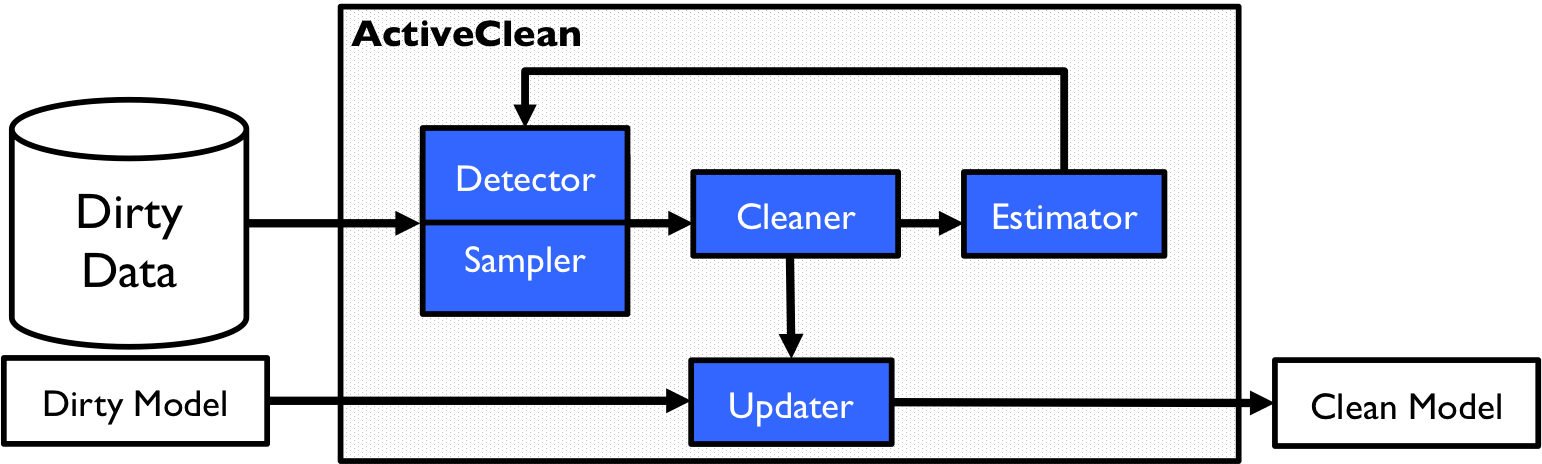
\includegraphics[width=\columnwidth]{figs/arch.png}
 \caption{\sysfull is an architecture where data cleaning is integrated with model training in a framework with sampling, model update, and feedback through estimation. \label{sys-arch}}\vspace{-2em}
\end{figure}

We propose \sys to address the progressive data cleaning problem in a way that avoids the three challenges: mixing, sampling, and sparsity.
The key insight is that an important class of predictive models, called convex loss models (e.g., linear regression and SVMs), are trained by iteratively drawing random samples of data and updating a model\cite{bertsekas2011incremental}.
Rather than happening before model training, Data cleaning can be directly integrated with the sampling and updating training process; preserving the same provable guarantees such as convergence and error bounds.
In \sys, data are cleaned in small random batches and the model is incrementally updated based on the results.
Similar to Active Learning, \sys selects the most valuable records to clean with higher probability, however, it applies a number of optimizations that exploit the data cleaning setting such as avoiding data that is expected to be clean, estimating of the effect of data cleaning for a record, and batching together updates from already cleaned data.
This framework is optimized for problems requiring expensive data cleaning.

The \sys architecture (Figure \ref{sys-arch}) consists of a \emph{detector}, \emph{sampler}, \emph{cleaner}, \emph{updater}, and \emph{estimator}.
The cleaner is an existing data cleaning framework (e.g., Entity Resolution), and \sys provides the remaining components to apply this framework progressively.
To summarize the contributions in each component:
\begin{itemize}[noitemsep]
\item Detector (Section \ref{det}). The detector can apply rules from data quality constraints or adaptively learn which records are dirty to increase the fraction of dirty records sampled.
\item Sampler (Section \ref{dist-samp}). We derive an optimal sampling distribution that minimizes the update variance (i.e., how different would the update be if another sample was drawn) which linearly improves an error bound on the convergence rate.
\item Updater (Section \ref{model-update}). The updater applies a weighted stochastic gradient descent step to the current best model. This update converges if all of the data is cleaned, and for batch size $b$ and iterations $T$, converges with rate $O(\frac{1}{\sqrt{bT}})$. 
\item Estimator (Section \ref{sampling}) The estimator applies a Taylor Series linearization to decouple changes in different features using knowledge about what is wrong with the data to better estimate the impact of an error.
\item The experiments evaluate these components on 4 datasets with real and synthetic corruption (Section \ref{eval}). The results suggest that indeed \sys is better suited for cleaning and model training when $k\ll N$. For a 5\%  systematic corruption, to achieve the same accuracy as a state-of-the-art Active Learning algorithm cleaning 1000 records, \sys cleans 55\% fewer records.
\end{itemize}







%\section{Problem Formalization}\label{statements}
\noindent This section formalizes the problems addressed in the paper.

\subsection{Notation and Setup}\label{notation}
The user provides a relation $R$, a cleaner $C(\cdot)$, a featurizer $F(\cdot)$, and a convex loss problem defined by the loss $\phi(\cdot)$.
A total of $k$ records will be cleaned in batches of size $b$, so there will be $\frac{k}{b}$ iterations. 
We use the following notation to represent relevant intermediate states:
\begin{itemize}[noitemsep]
\item \textbf{Dirty Model: } $\theta^{(d)}$ is the model trained on $R$ (without cleaning) with the featurizer $F(\cdot)$ and loss $\phi(\cdot)$. This serves as an initialization to \sys.
\item \textbf{Dirty Records: } $R_{dirty} \subseteq R$ is the subset of records that are still dirty. As more data are cleaned $R_{dirty} \rightarrow \{\}$.
\item \textbf{Clean Records: } $R_{clean} \subseteq R$ is the subset of records that are clean, i.e., the complement of $R_{dirty}$.
\item \textbf{Samples: } $S$ is a sample (possibly non-uniform but with known probabilities) of the records $R_{dirty}$. The clean sample is denoted by $S_{clean} = C(S)$.
\item \textbf{Clean Model: } $\theta^{(c)}$ is the optimal clean model, i.e., the model trained on a fully cleaned relation.
\item \textbf{Current Model: } $\theta^{(t)}$ is the current best model at iteration $t \in \{1,...,\frac{k}{b}\}$, and $\theta^{(0)} = \theta^{(d)}$. 
\end{itemize}

There are two metrics that we will use to measure the performance of \sys:

\vspace{0.25em}

\noindent\textbf{Model Error. } The model error is defined as $\|\theta^{(t)} - \theta^{(c)}\|$.

\vspace{0.25em}

\noindent\textbf{Testing Error. } Let $T(\theta^{(t)})$ be the out-of-sample testing error when the current best model is applied to the clean data, and $T(\theta^{(c)})$ be the test error when the clean model is applied to the clean data. The testing error is defined as $T(\theta^{(t)}) - T(\theta^{(c)})$

\subsection{Problem 1. Correct Update Problem}\label{updp}
Given newly cleaned data $S_{clean}$ and the current best model $\theta^{(t)}$, the model update problem is to calculate $\theta^{(t+1)}$. 
$\theta^{(t+1)}$ will have some error with respect to the true model $\theta^{(c)}$, which we denote as:
\[
error(\theta^{(t+1)}) = \| \theta^{(t+1)} - \theta^{(c)} \|
\]
Since a sample of data are cleaned, it is only meaningful to talk about expected errors.
We call the update algorithm ``reliable" if the expected error is upper bounded by a monotonically decreasing function $\mu$ of the amount of cleaned data:
\[
\mathbb{E}(error(\theta^{new})) = O(\mu(\mid S_{clean} \mid))
\]
Intuitively, ``reliable" means that more cleaning should imply more accuracy.

\vspace{0.5em}

\emph{The Correct Update Problem is to reliably update the model $\theta^{(t)}$ with a sample of cleaned data.}

\subsection{Problem 2. Efficiency Problem}\label{optp}
The efficiency problem is to select $S_{clean}$ such that the expected error $\mathbb{E}(error(\theta^{(t)}))$ is minimized.
\sys uses previously cleaned data to estimate the value of data cleaning on new records.
Then it draws a sample of records $S \subseteq R_{dirty}$. 
This is a non-uniform sample where each record $r$ has a sampling probability $p(r)$ based on the estimates.
We derive the optimal sampling distribution for the SGD updates, and show how the theoretical optimum can be approximated.

\vspace{0.5em}

\emph{The Efficiency Problem is to select a sampling distribution $p(\cdot)$ over all records such that the expected error w.r.t to the model if trained on fully clean data is minimized.}

\iffalse
\subsection{\sys Problem}
The core problem addressed by \sys is incremental model update while progressively cleaning data.

\begin{problem}[ActiveClean Problem]\label{activeclean}\sloppy
Let $R$ be a dirty relation, $F(r) \mapsto (x,y)$ be a featurization that maps
a record $r \in R$ to a feature vector $x$ and label $y$, $\phi$ be a convex regularized loss,
and $C(r) \mapsto r_{clean}$ be a cleaning technique that maps a record to its cleaned value. 
Given these inputs, the \sys problem is to return a \textbf{reliable} estimate $\hat{\theta}$ of the clean model for any limit $k$ on the number of times the data cleaning $C(\cdot)$ can be applied.

\vspace{0.5em}

\textbf{Reliable} precisely means that the expected error in this estimate (i.e., L2 difference w.r.t a model trained on a fully cleaned dataset) is bounded above by a monotonic function in $k$ and a monotonic function of the error in the dirty model.
\end{problem}
\fi


\iffalse
From a systems perspective, data cleaning and model training happen at very different time scales.
When humans are involved, per record latencies for data cleaning are orders of magnitude larger than the CPU time needed for model training.
We can compare recent results in data cleaning to a model training framework like CoCoA implemented on Spark \cite{jaggi2014communication}.
Per record, BigDansing, a highly optimized automated Spark-based data cleaning system is 15.5x slower than CoCoA\footnote{For CoCoA to reach a precision of 1e-3}.
Crowd based techniques like CrowdFill \cite{park2014crowdfill} and CrowdER \cite{wang2012crowder} are over 100,000x slower per record. 
Consequently, all of the optimizations in \sys are designed to address data cleaning latency (i.e., more progress with fewer cleaned records) rather than optimizing for numerical computation (i.e., process fewer records).
\fi



\iffalse
Here is an example application of \sys with our running example:
\begin{example}
The analyst first trains her SVM model on the dirty data ignoring the effects of the errors returning a model $\theta^{(d)}$.
She decides that she has a budget of cleaning $100$ records, and decides to clean the 100 records in batches of 10 (set based on how fast she can clean the data, and how often she wants to see an updated result).
She initializes \sys with $\theta^{(d)}$.
\sys samples an initial batch of 10 records.
She manually cleans those records by merging similar drug names, making corporation names consistent, and fixing incorrect labels.
After each batch, the model is updated with the most recent cleaning results $\theta^{(t)}$.
The model improves after each iteration.
After $t=10$ of cleaning, the analyst has an accurate model trained with 100 cleaned records but still utilizes the entire dirty data.
\end{example}



\subsection{Two perspectives on error}
When faced with such errors there are two contrasting perspectives from the Machine Learning and the Database communities.

\vspace{0.5em}

\noindent\textbf{Existing Database Literature. } 
Traditionally, cleaning is agnostic to the queries and analysis that happens downstream. 
This perspective breaks down when cleaning is so expensive that we can only clean a small number of records.
Ideally, we should clean the records that are most valuable to the downstream analysis.

\vspace{0.5em}

\noindent\textbf{Existing  Machine Learning Literature. } The Machine Learning community has focused on
designing models that are robust to outliers (i.e., values far away from the typical value)
For example, in the case of linear regression, we can change the $L_2$ norm to an $L_1$ norm to mitigate the effect of outliers:
\[
\phi(x_{i}^T\theta,y_{i}) = \|\theta^Tx_{i} - y_i \|_1
\]
The quadratic L2 loss implies that examples that deviate far from the typical example are quadratically penalized as opposed to linearly penalized with the L1 loss.
There is a natural tradeoff between robustness and efficiency.
The more robust a technique is, the less efficient it will be (i.e., estimate variance for a fixed number of training examples).
Robust techniques are best suited for random errors that look significantly different the rest of the examples.
When errors are systematic, the Machine Learning answer has been to design features in such a way that they are robust to some systematic bias.
For example, in image processing, scale-invariant feature transforms (SIFT) are widely applied that allow for image models invariant to pose or scaling issues.

\vspace{0.5em}

\noindent\textbf{The \sys Contribution. } We try to bring two perspectives together in this work to address the problem of expensive to clean systematic errors, namely the Database idea of data cleaning and the Machine Learning formalization of empirical risk minimization.
Some errors require expensive cleaning procedures, increasingly using the crowd, and we joint have a time budget on cleaning and analysis.
\sys prioritizes cleaning with respect to an estimated impact on the clean model.

\subsection{SampleClean Project}

Traditionally, data cleaning has explored expensive, up-front cleaning of entire datasets for increased query accuracy.
We proposed the SampleClean problem, in which an analyst cleans a small sample of data, and then estimates the result to an aggregate query e.g., \sumfunc, \countfunc, or \avgfunc.
The main insight from the SampleClean project is that highly accurate answers for aggregate queries does not require cleaning the full dataset.
Generalizing this insight, there is a deep relationship between the application (i.e., the query) and how an analyst should budget their effort in data cleaning.
In fact, \avgfunc and \sumfunc queries are a special case of the convex loss minimization discussed in the previous section:
\[
\phi = (x_{i} - \theta)^2
\]

We then extended the SampleClean work to study cleaning Materialized Views \cite{technicalReport}.
Suppose base data is updated with insertions, deletions, or updates, we explored how we could efficiently propagate
changes to a sample of the view instead of the full view.
Subsequent queries on the view could be answered approximate.

The SampleClean problem inspired an eponymous system that implements sampling, data cleaning, and approximate query processing on the Apache Spark stack \cite{sampleclean}.
Also included in the Apache Spark stack are Machine Learning libraries including MLlib \cite{mllib} and GraphX \cite{graphx}.
The in-memory architecture of the Apache Spark stack allows for increasingly interactive analysis \cite{AgarwalMPMMS13, armbrust2015spark}.
Analysts can prototype data processing workflows on samples to evaluate performance before running expensive batch processing jobs on entire datasets.
With data cleaning and machine learning libraries in the same software ecosystem, we see a new opportunity for joint optimization for interactive model building.



\subsection{Stochastic Gradient Descent}
Sampling is a natural part of any Machine Learning workflow, as stochastic optimization is widely used to fit model parameters.
The problems described in the previous subsections are often trained using a technique called Stochastic Gradient Descent (SGD) or one of its variants.
The basic idea of SGD is to draw a data point at random, calculate the gradient at that point, and then update a current best estimate with that gradient.
\[
\theta^{(t+1)}\leftarrow\theta^{(t)}-\gamma\nabla\phi(x_{i}^T\theta,y_{i})
\]
 SGD can also be applied in a ``mini-batch" mode, where we draw a subset of data $S^{(t)}$ at random and update with the average gradient.
 \[
 \theta^{(t+1)}\leftarrow\theta^{(t)}-\frac{\gamma}{\|S^{(t)}\|}\sum_{i\in S^{(t)}}\nabla\phi(x_{i}^T\theta,y_{i})
 \]

We can use this workflow for designing an anytime data cleaning methodology.
As data is sampled, we can clean the samples.
The analyst then can stop at anytime and use the best model at that instant.
SGD and its variants are well-studied and there are lower-bounds on the convergence rates using these techniques. 
Recently, a number of works have explored non-uniform sampling distributions for stochastic optimization \cite{zhao2014stochastic, qu2014randomized}.
The main insight is that non-uniform distributions may on average estimate the gradient accurately.
In this work, we explore how to design such a non-uniform distribution for iterative data cleaning.

\fi


 

%\section{System Architecture}\label{arch}
This section describes the \sys architecture and the basic algorithmic framework.
The individual components will be addressed in the subsequent sections.

\subsection{Overview}
Figure \ref{sys-arch}, in the introduction, overviews the entire framework.
The first step of \sys is \emph{initialization}.
In this step, there is a dirty relation $R$, a featurization $F(\cdot)$, a data cleaning technique $C(\cdot)$, and a dirty model $\theta^{(d)}$ trained on the featurized dirty relation. 
Optionally, \sys integrates with dirty data detection rules $D(\cdot)$ which selects the set of likely corrupted records from $R$.
If one is not provided, \sys starts by treating all of the data as dirty and tries to learn a detector as data are cleaned.
At initialization, there are two hyperparameters to set, the cleaning budget $k$ and the batch size $b$ (the number of iterations is $T = \frac{k}{b}$).
We discuss how to set $b$ and the tradeoffs in setting a larger or smaller $b$ in Section \ref{model-update}.

After initialization, \sys begins the cleaning and model update iterations.
The \emph{sampler} selects a sample of dirty data based on the batch size.
At this step, \sys can use the detector $D$ to narrow the sample to likely dirty data.
Once a sample is selected, the \emph{cleaner} applies $C(\cdot)$ to the dirty sample.
%Then, after the sample is cleaned, the current model is updated.
\sys is initialized with the dirty model, and this model is iteratively updated as more batches are cleaned.

The next two steps in the architecture are feedback steps where the sampling distribution is updated for the next iteration.
The \emph{estimator} uses previously cleaned data to estimate the value of data cleaning on new records.
This information is used to guide sampling towards more valuable records.
After estimation, the detector $D(\cdot)$ is also updated based on cleaned data.
After all of the iterations are complete, the system returns the updated model.

To summarize the architecture in pseudocode:
\begin{enumerate}[leftmargin=1em]\scriptsize\sloppy
\item \texttt{Init(dirty\_data, cleaned\_data, dirty\_model, batch, iter)}
\item For each t in $\{1,...,T\}$
\begin{enumerate}
	\item \texttt{dirty\_sample $=$ Sampler(dirty\_data, sample\_prob, detector, batch)}
	\item \texttt{clean\_sample $=$ Cleaner(dirty\_sample)}
	\item \texttt{current\_model $=$ Update(current\_model, sample\_prob, clean\_sample)}
	\item \texttt{cleaned\_data = cleaned\_data + clean\_sample}
	\item \texttt{dirty\_data = dirty\_data - clean\_sample}
	\item \texttt{sample\_prob $=$ Estimator(dirty\_data, cleaned\_data, detector)}
	\item \texttt{detector $=$ DetectorUpdater(detector, cleaned\_data)}
\end{enumerate}
\item \texttt{Output: current\_model}
\end{enumerate}

Here is an example application of \sys:
\begin{example}
The analyst first trains an SVM model on the dirty data ignoring the effects of the errors resulting in a model $\theta^{(d)}$.
She decides that she has a budget of cleaning $100$ records, and decides to clean the 100 records in batches of 10 (set based on how fast she can clean the data, and how often she wants to see an updated result).
She initializes \sys with $\theta^{(d)}$.
\sys samples an initial batch of 10 records.
She manually cleans those records by merging similar drug names, making corporation names consistent, and fixing incorrect labels.
After each batch, the model is updated with the most recent cleaning results $\theta^{(t)}$.
The model improves after each iteration.
After $t=10$ of cleaning, the analyst has an accurate model trained with 100 cleaned records but still utilizes the entire dirty data.
\end{example}

\subsection{Challenges and Formalization}
We highlight the important components and formalize the research questions explored in this paper. 

\vspace{0.5em}

\noindent\textbf{Detector (Section \ref{det}). } The first challenge in \sys is dirty data detection. In this step, the detector select a candidate set of dirty records $R_{dirty} \subseteq R$. There are two techniques to do this: (1) an \emph{a priori} case, and (2) and an adaptive case. In the \emph{a priori} case, the detector knows which data is dirty in advance. In the adaptive case, the detector learns classifier based on previously cleaned data to detect corruption in uncleaned data.

\vspace{0.5em}

\noindent\textbf{Sampler (Section \ref{dist-samp}). } The sampler draws a sample of records $S_{dirty} \subseteq R_{dirty}$. This is a non-uniform sample where each record $r$ has a sampling probability $p(r)$.
We will derive the optimal sampling distribution, and show how the theoretical optimal can be approximated by the next estimator.

\vspace{0.5em}

\noindent\textbf{Cleaner (User-Specified). } Given the sample of the records $S_{dirty}$,  the cleaner applies the user-specified data cleaning $C(\cdot)$. This paper focuses on a record-by-record cleaning model where the function $C$ is applied to a record and produces the clean record:
\[
S_{clean} = \{C(r) : \forall r \in S_{dirty}\}
\]
This allows for uniform measure of the performance of \sys in terms of model error as a function of sample size. The record-by-record cleaning model is not a fundamental restriction of this approach, and in the extensions (Section \ref{set-of-r}), there is a discussion on a compatible ``set of records" cleaning model. Consider the case where an analyst finds a dirty record, and is able to fix all records (possibly outside the sample) the with same error throughout the dataset efficiently.

\vspace{0.5em}

\noindent\textbf{Update (Section \ref{model-update}). } This step updates the model $\theta^{(t)}$ based on the featurized (with featurization $F(\cdot)$) cleaned sample $F(S_{clean})$ resulting in $\theta^{(t+1)}$. Analyzing the model update procedure as a stochastic gradient descent algorithm will help derive the sampling distribution and estimation.

\vspace{0.5em}

\noindent\textbf{Estimator (Section \ref{sampling}): } The estimator approximates the optimal distribution derived in the Sample step. Based on the change in the featurized data $F(S_{clean})$ and $F(S_{dirty})$, it directs the next iteration of sampling to select points that will have changes most valuable to the next model update.

\iffalse
\subsection{Optimizations}
There are three aspects of \sys, that allow us to achieve this design point: error partitioning, gradient-based model update (Section \ref{model-update}), estimate-driven sampling (Section \ref{sampling}).

\vspace{0.5em}

\noindent\textbf{Partitioning Dirty and Clean Data: } In many applications, enumerating the set of corrupted records is much easier than cleaning them. For example, we may be able to select the set of rows that have missing values but actually filling those missing values is expensive. Likewise, in the constraint literature, selecting a set of rows that have a violated constraint can be done in polynomial time, however, fixing the constraints is NP-Hard.
In our error detection step, we partition the dirty and clean data.
Partitioning serves two purposes: (1) it reduces the variance of our updates because we can cheaply scan over data we know that is clean, and (2) it increases the fraction of actually dirty records in the candidate batch.
A good example of why we need the second objective is seen in the context of crowdsourcing.
If we have a crowdworker clean records, we will have to pay them for the task whether or not the record required cleaning.
To efficiently use this partitioning, we need a database solution indexing dirty and clean data.

\vspace{0.5em}

\noindent\textbf{Gradient-Based Updates: } In \sys, we start with a dirty model and then make an update using a gradient step. Here, we can draw an analogy to Materialized View maintenance, since after all, a model parametrized by $\theta$ is just a table of floating point numbers.
Krishnan et al. proposed a technique called sample view cleaning, in which they take a clean sample of data and propagate the updates to a Materialized View.
Similarly, in this work, we take the information from a sample of cleaned data and propagate an update with the gradient.

\vspace{0.5em}

\noindent\textbf{Estimate-Driven Sampling: } Repair is the most expensive step in the workflow, so optimizing for scan cost may lead to negligible overall time improvements.
We can sacrifice a small overhead in pre-computation for each data point to determine its value to the model and select a sampling distribution accordingly.
Intuitively, while each iteration has an increased cost, it also makes more progress towards the optimum.
\fi



%\input{correction.tex}
%\input{delta.tex}
%\section{Selecting Records to Clean}\label{dist-samp}
The algorithm proposed in Section \ref{update-alg} will convege for 
any sampling distribution where  $p(\cdot) > 0$ for all records, albeit different distributions will have different convergence rates.
The sampling algorithm is designed to include records in each batch that are most valuable to the analyst's model with a higher probability.

\subsection{Optimal Sampling Problem}
Recall that the convergence rate of an SGD algorithm is bounded by $\sigma^2$ which is the variance of the gradient.
Intuitively, the variance measures how accurately the gradient is estimated from a uniform sample.
Other sampling distributions, while preserving the same expected value, may have a lower variance.
Thus, the optimal sampling problem is defined as a search over sampling distributions to find the minimum variance sampling distribution.

\begin{definition}[optimal Sampling Problem]
Given a set of candidate dirty data $R_{dirty}$, $\forall r \in R_{dirty}$ find sampling probabilities $p(r)$ such that over all samples $S$ of size $k$ it minimizes the variance:
\[
\arg\min_p \mathbb{E}(\|g_S - g^*\|^2)
\]
\end{definition}

It can be shown~\cite{zhao2014stochastic} that the optimal distribution over records in $R_{dirty}$ is proportional to: $p_i \propto \|\nabla\phi(x^{(c)}_i,y^{(c)}_i,\theta^{(t)})\|$
Intuitively, this sampling distribution prioritizes records with higher gradients, i.e., make a larger impact during optimization.
The challenge is that this particular optimal distribution depends on knowing the clean value of a records, which is a chicken-and-egg problem:
the optimal sampling distribution requires knowing $(x^{(c)}_i,y^{(c)}_i)$; however, we are sampling the values so that they can be cleaned.

One natural solution is to calculate this gradient with respect to the dirty values--implicitly assuming that the corruption is not that severe:
\[
p_i \propto \|\nabla\phi(x^{(d)}_i,y^{(d)}_i,\theta^{(t)})\|
\]
This solution is highly related to the Expected Gradient Length heuristic that has been proposed before in Active Learning\cite{settles2010active}.
However, there is additional structure to the data cleaning problem.
As the analyst cleans more data, we can build a model for how cleaned data relates to dirty data.
By using the detector from the previous section to estimate the impact of data cleaning, we show that we can estimate the cleaned values.
We find that this optimization can improve the convergence rate by a factor of 2 in some datasets.
%Note that as long as every record gets sampled, the algorithm will still converge.





%\input{correction2.tex}
%\input{outlier.tex}
%\input{analysis.tex}
%\section{Experiments}
There are a number of different axes on which we can evaluate \sys.
First, we take real datasets and generate various types of errors to illustrate the value of data cleaning in comparison to robust statistical techniques.
Next, we explore different prioritization and model update schemes for data cleaning samples.
Finally, we evaluate \sys end-to-end in a number of real-world data cleaning scenarios.

\subsection{Experimental Setup and Notation}
Every experiment has two steps: data cleaning and model evaluation.
We evaluate the data cleaning on one metric:

\noindent\textbf{Cleaning Efficiency. } Let $K$ be the number of samples processed by the algorithm, and $K'$ be the number of samples that were actually dirty. The cleaning efficiency is $\frac{K'}{K}$.

In our experiments, we explore three classification models: L1-Hinge Loss SVM, Logistic Regression, and Thresholded Linear Regression.
We evaluate the trained models on the following metrics:

\noindent\textbf{Relative Model Error. } Let $\theta$ be the model trained on the dirty data, and let $\theta^*$ be the model trained on the same data if it was cleaned. Then the model error is defined as $\frac{\|\theta - \theta^*\|}{\|\theta^*\|}$.

\noindent\textbf{Testing Accuracy. } Let $\theta$ be the model trained on the dirty data, and let $\theta^*$ be the model trained on the same data if it was cleaned. Let $T(\theta)$ be the out-of-sample testing accuracy when the dirty model is applied to the clean data, and $T(\theta^*)$ be the testing accuracy when the clean model is applied to the clean data. The testing error is defined as $T(\theta^*) - T(\theta)$

\subsubsection{Scenarios}
We apply these models in the following scenarios:

\noindent\textbf{Housing: } In this dataset, our task is to predict housing prices from 13 numerical and categorical covariates. There are 550 data points in this dataset. The model is a Logistic Regression classifier which predicts if the house price is greater than \$500k.

\noindent\textbf{Adult: } In this census dataset, our task is to predict the income bracket (binary) from 12 numerical and categorical covariates. There are 45552 data points in this dataset. We use a SVM classifier to predict the income bracket of the person.

\noindent\textbf{EEG: } In this dataset, our task is to predict the on set of a seizure (binary) from 15 numerical covariates. There are 14980 data points in this dataset. This dataset is unique because the classification is hard with linear predictors. The model that we use is a thresholded Linear Regression.

\noindent\textbf{MNIST: } In this dataset, our task is to classify 60,000 images of handwritten images into 10 categories. The unique part of this dataset is the featurized data consists of a 784 dimensional vector which includes edge detectors and raw image patches. We use this dataset to explore how we can corrupt the raw data to affect subsequent featurization. The model is an one-to-all multiclass SVM classifier. 

\subsection{Experiment 1. Effect of Cleaning}
Before we evaluate \sys, we first evaluate the benefits of cleaning on our 4 example datasets.
We first explore this problem without sampling to understand which types of errors are amenable to data cleaning and which are better suited for robust statistical techniques.
We compare 4 schemes: (1) cleaning, (2) adding an L2 regularizer tuned to maximal accuracy with a grid search, (3) discarding the dirty data, and (4) baseline of no cleaning.

We corrupted 5\% of the training examples in each dataset.
We corrupted these data in two different ways.

\noindent\textbf{Random errors: } We simulated high-magnitude random outliers. We select 5\% of the examples and features uniformly at random and replace a feature with 3 times the highest feature value.

\noindent\textbf{Systematic errors: } We simulated innocuous looking (but still incorrect) systematic errors. We trained the model on the clean data, find the most important feature (highest weighted). We sort examples but this feature and corrupt the top 5\% of examples with the mean value for that feature.

\begin{figure}[ht!]
\centering
 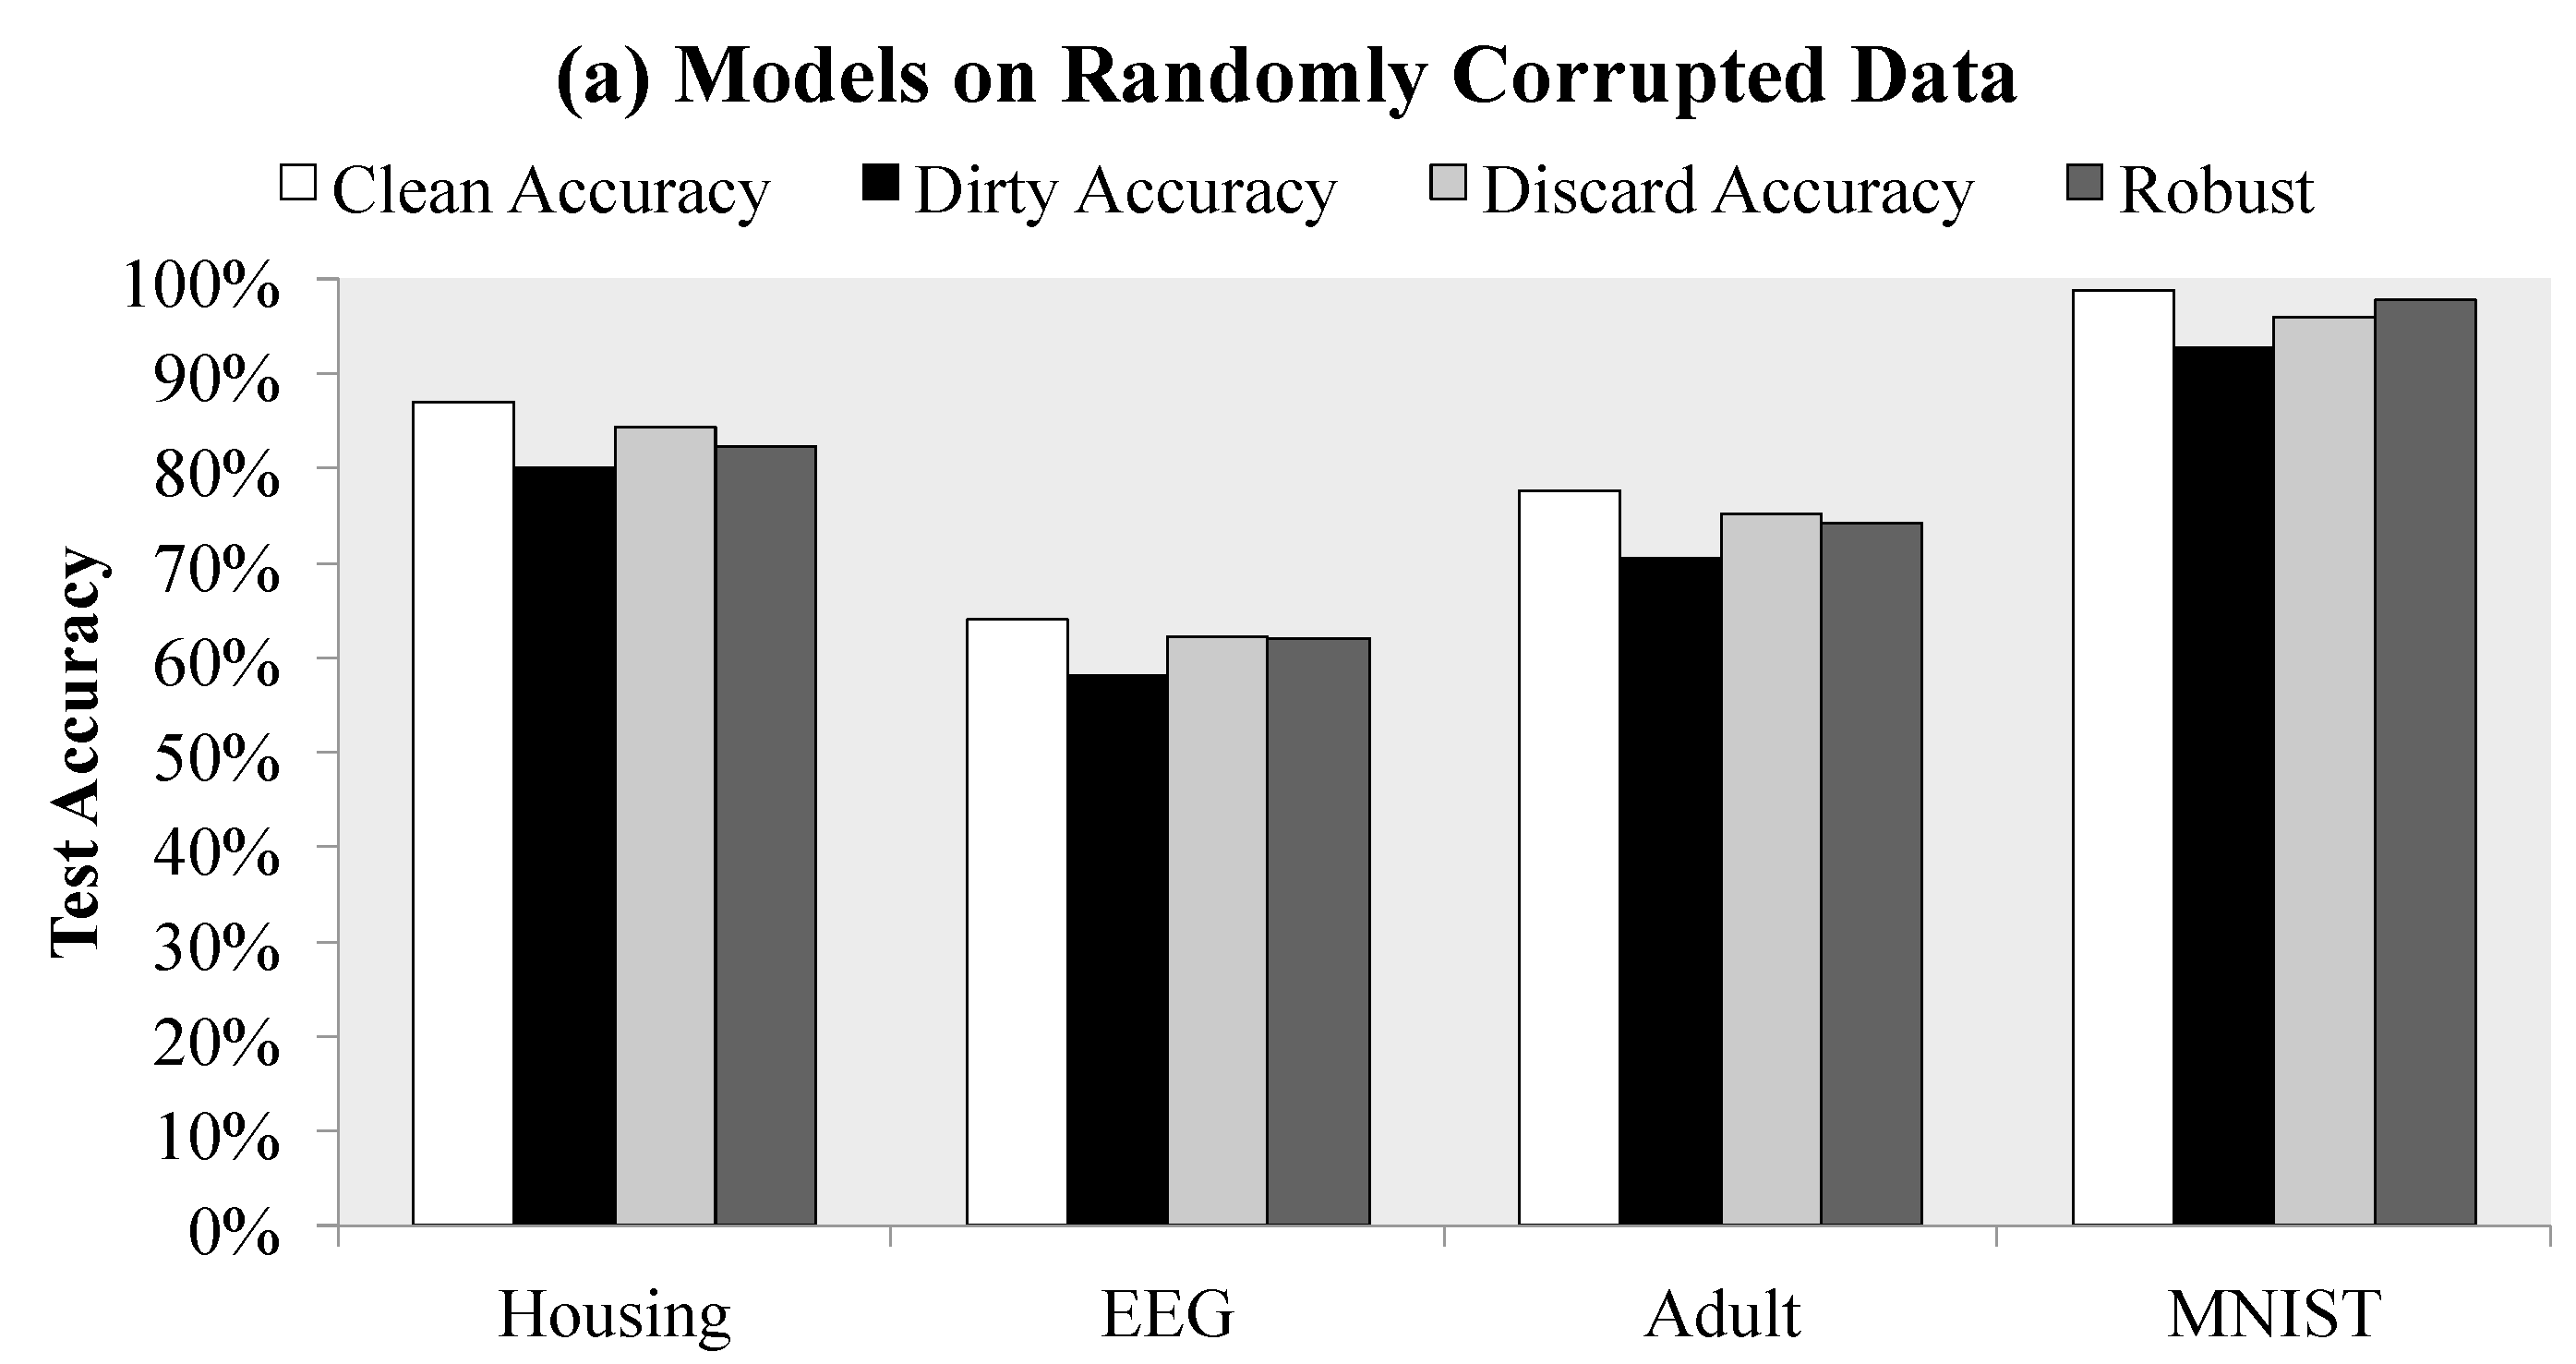
\includegraphics[width=0.8\columnwidth]{exp/exp2.pdf}
 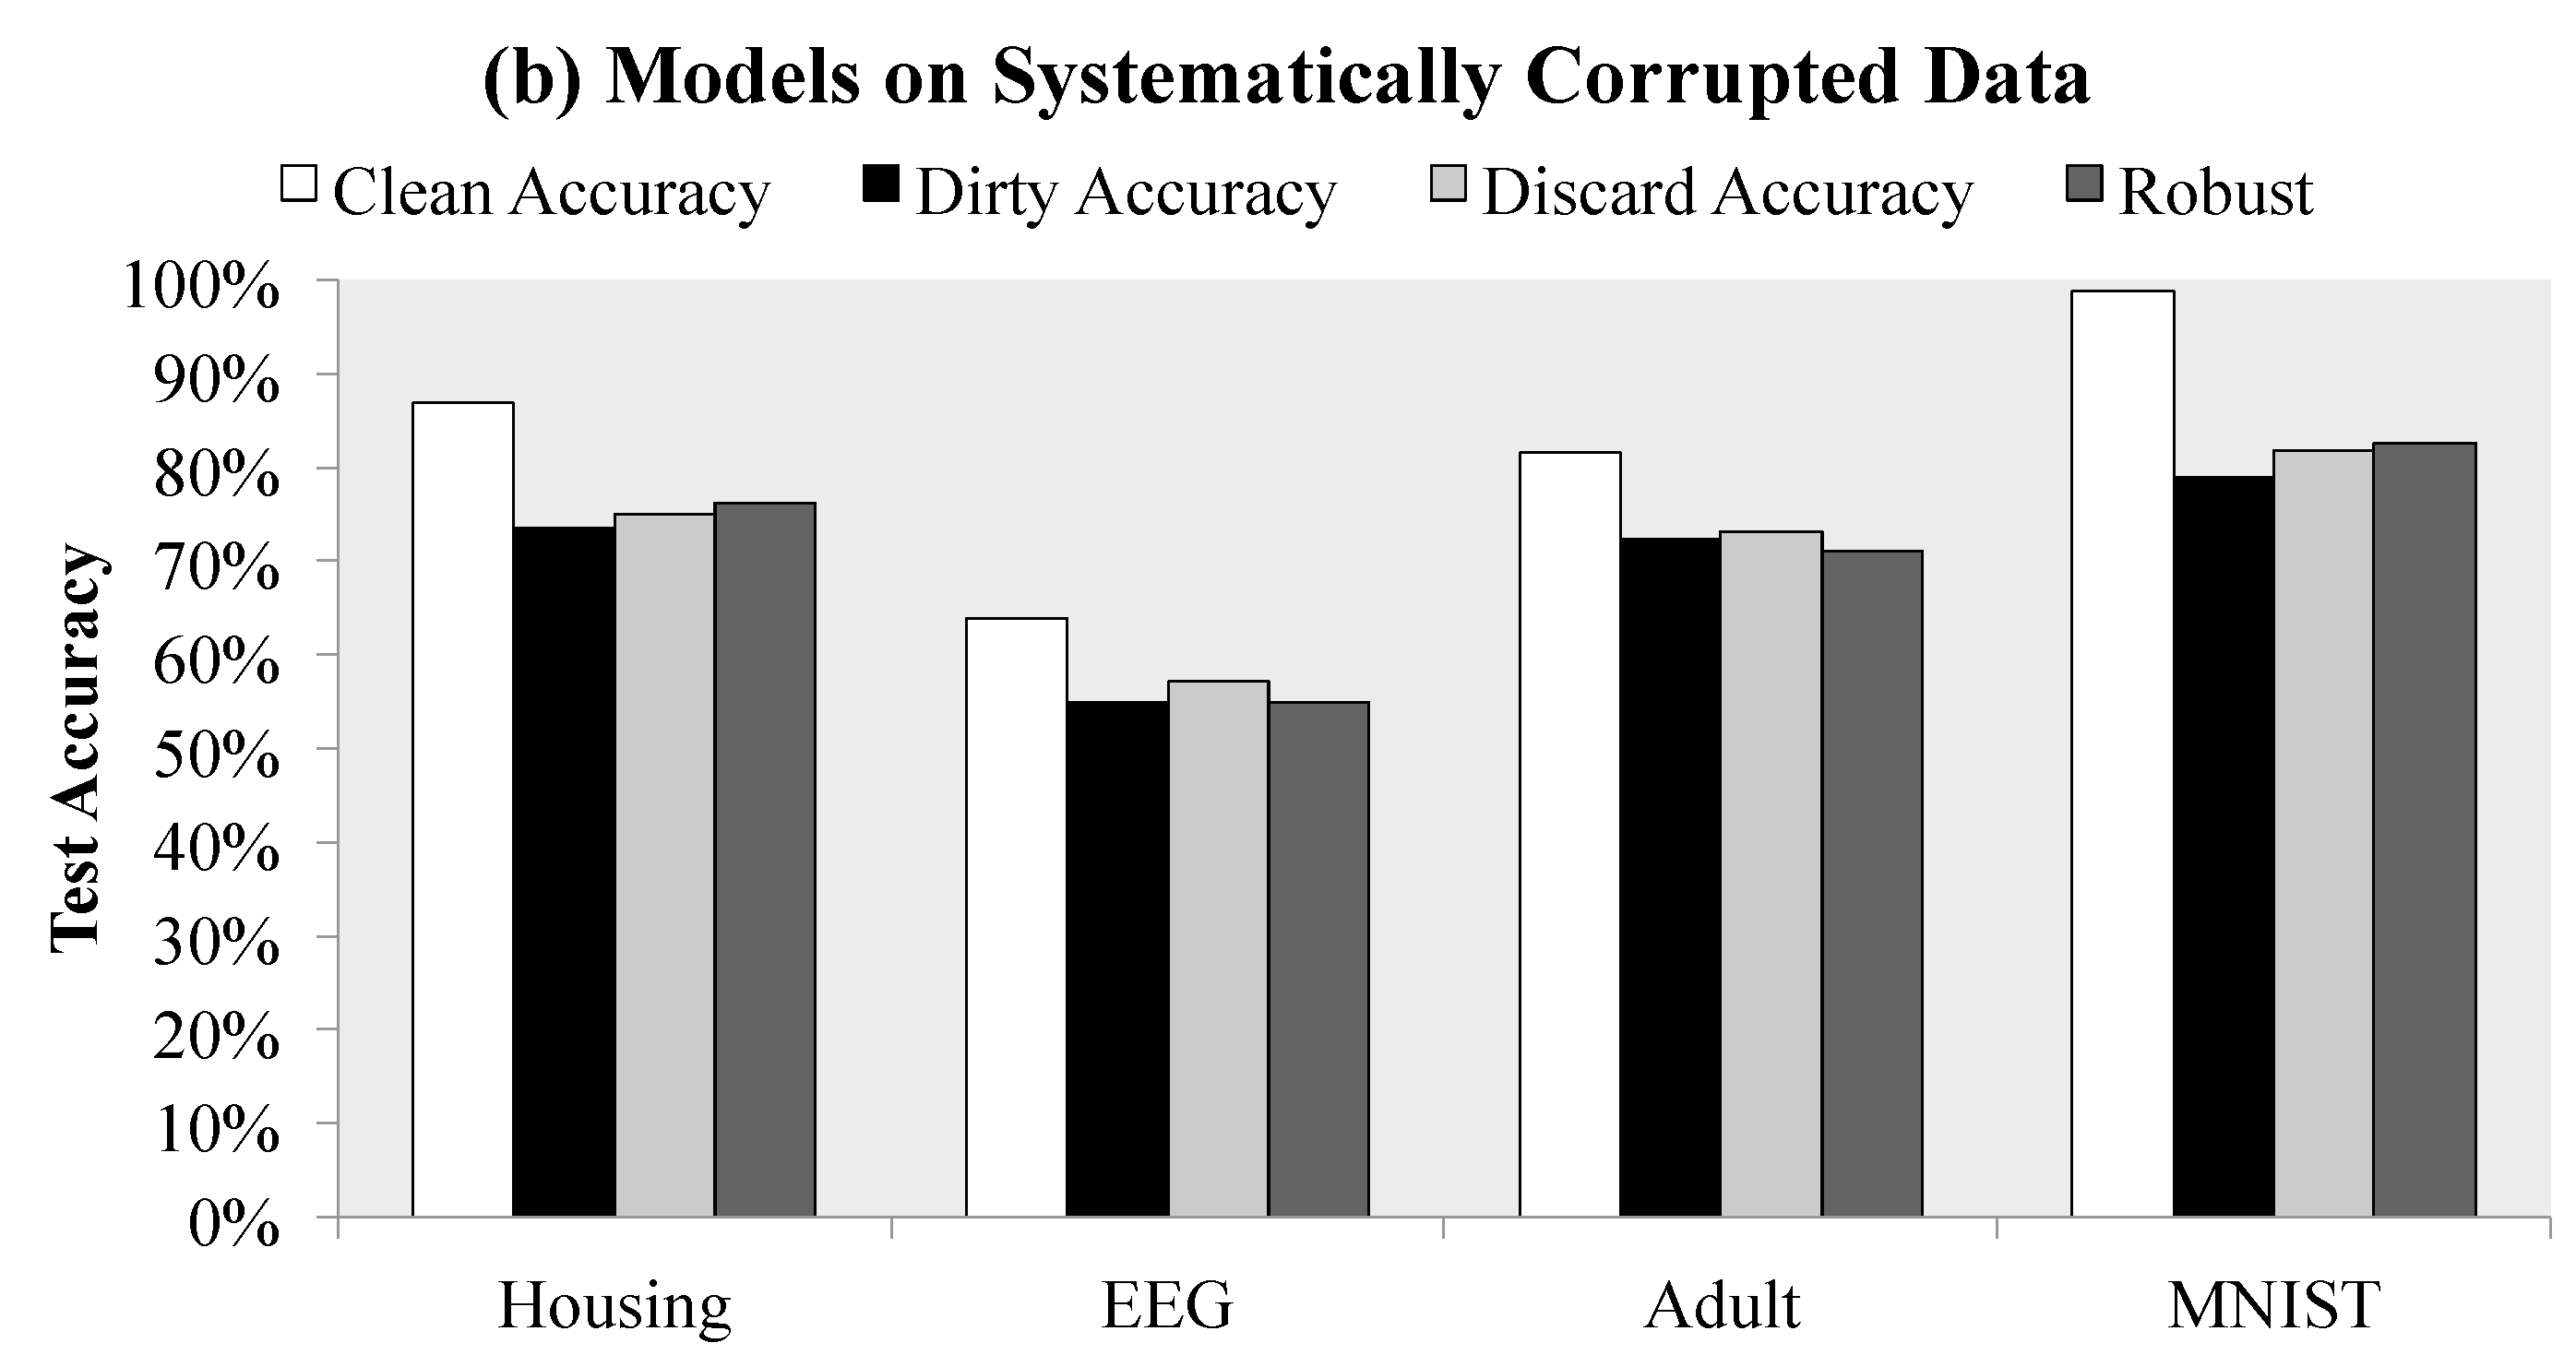
\includegraphics[width=0.8\columnwidth]{exp/exp1.pdf}
 \caption{Robust techniques work best when corrupted data are random and look atypical. Data cleaning can provide reliable performance in both the systematically corrupted setting and randomly corrupted setting.\label{sys-rand}}
\end{figure}

In Figure \ref{sys-rand}, we present the results of this experiment.
As we argued in this paper, the robust method performs well on the random high-magnitude outliers, however, falters on the systematic corruption.
Interestingly enough, in the random setting, discarding dirty data also performs well.
However, when errors are systematic data cleaning is the most reliable option across datasets.
In the MNIST dataset, we see a particularly significant effect of systematic corruption
where the test accuracy drops from nearly 98\% to 78\%.
Multiclass classification is particularly sensitive to systematic corruption when the corruptions can make classes ambiguous (e.g. reconizing a ``4" and a ``9").
The problem is that a priori, we do not know if data error is random or systematic.
While data cleaning requires more effort, it provides benefits in both settings.

\subsection{Experiment 2. Prioritization}
The next set of experiments evaluate different approaches to cleaning a sample of data.
In this set of experiments, we use the random errors generated above.

\subsubsection{2a. Alternative Algorithms}
In our first prioritization experiment, we evaluate the samples-to-error tradeoff between three alternative algorithms:

\noindent\textbf{SampleClean (SC): } In SampleClean, we do not use a gradient update and instead take a sample of data and train the model to completion on the sample.

\noindent\textbf{Active Learning (AL): } In Active Learning, we do not consider the effect of ``data cleaning" and prioritze points by their dirty gradient value. We do, however, do this iteratively and update the model.

\noindent\textbf{ActiveClean Oracle (AC+O): } In ActiveClean Oracle, we importance sample points by their clean gradient. This represents the theoretical best that our algorithm could hope to achieve given perfect error estimation.

In Figure \ref{prio-perf}, we present our results on Housing, Adult, and EEG. 
We find that \sys gives its largest benefits for small sample sizes (up-to 12x).
\sys makes significant progress because of its intelligent initialization, iterative updates, and partitioning.
For example, the EEG dataset is the hardest classification task.
SampleClean has difficulty on this dataset since it takes a uniform sample of data (only 5\% of which are corrupted on average) and tries to train a model using only this data.
\sys and Active Learning leverage the initialization from the dirty data to get an improved result. 
However, \sys's impact estimates and error partitioning allow us to beat Active Learning on all three of the datasets.

\begin{figure*}[t]
\centering
 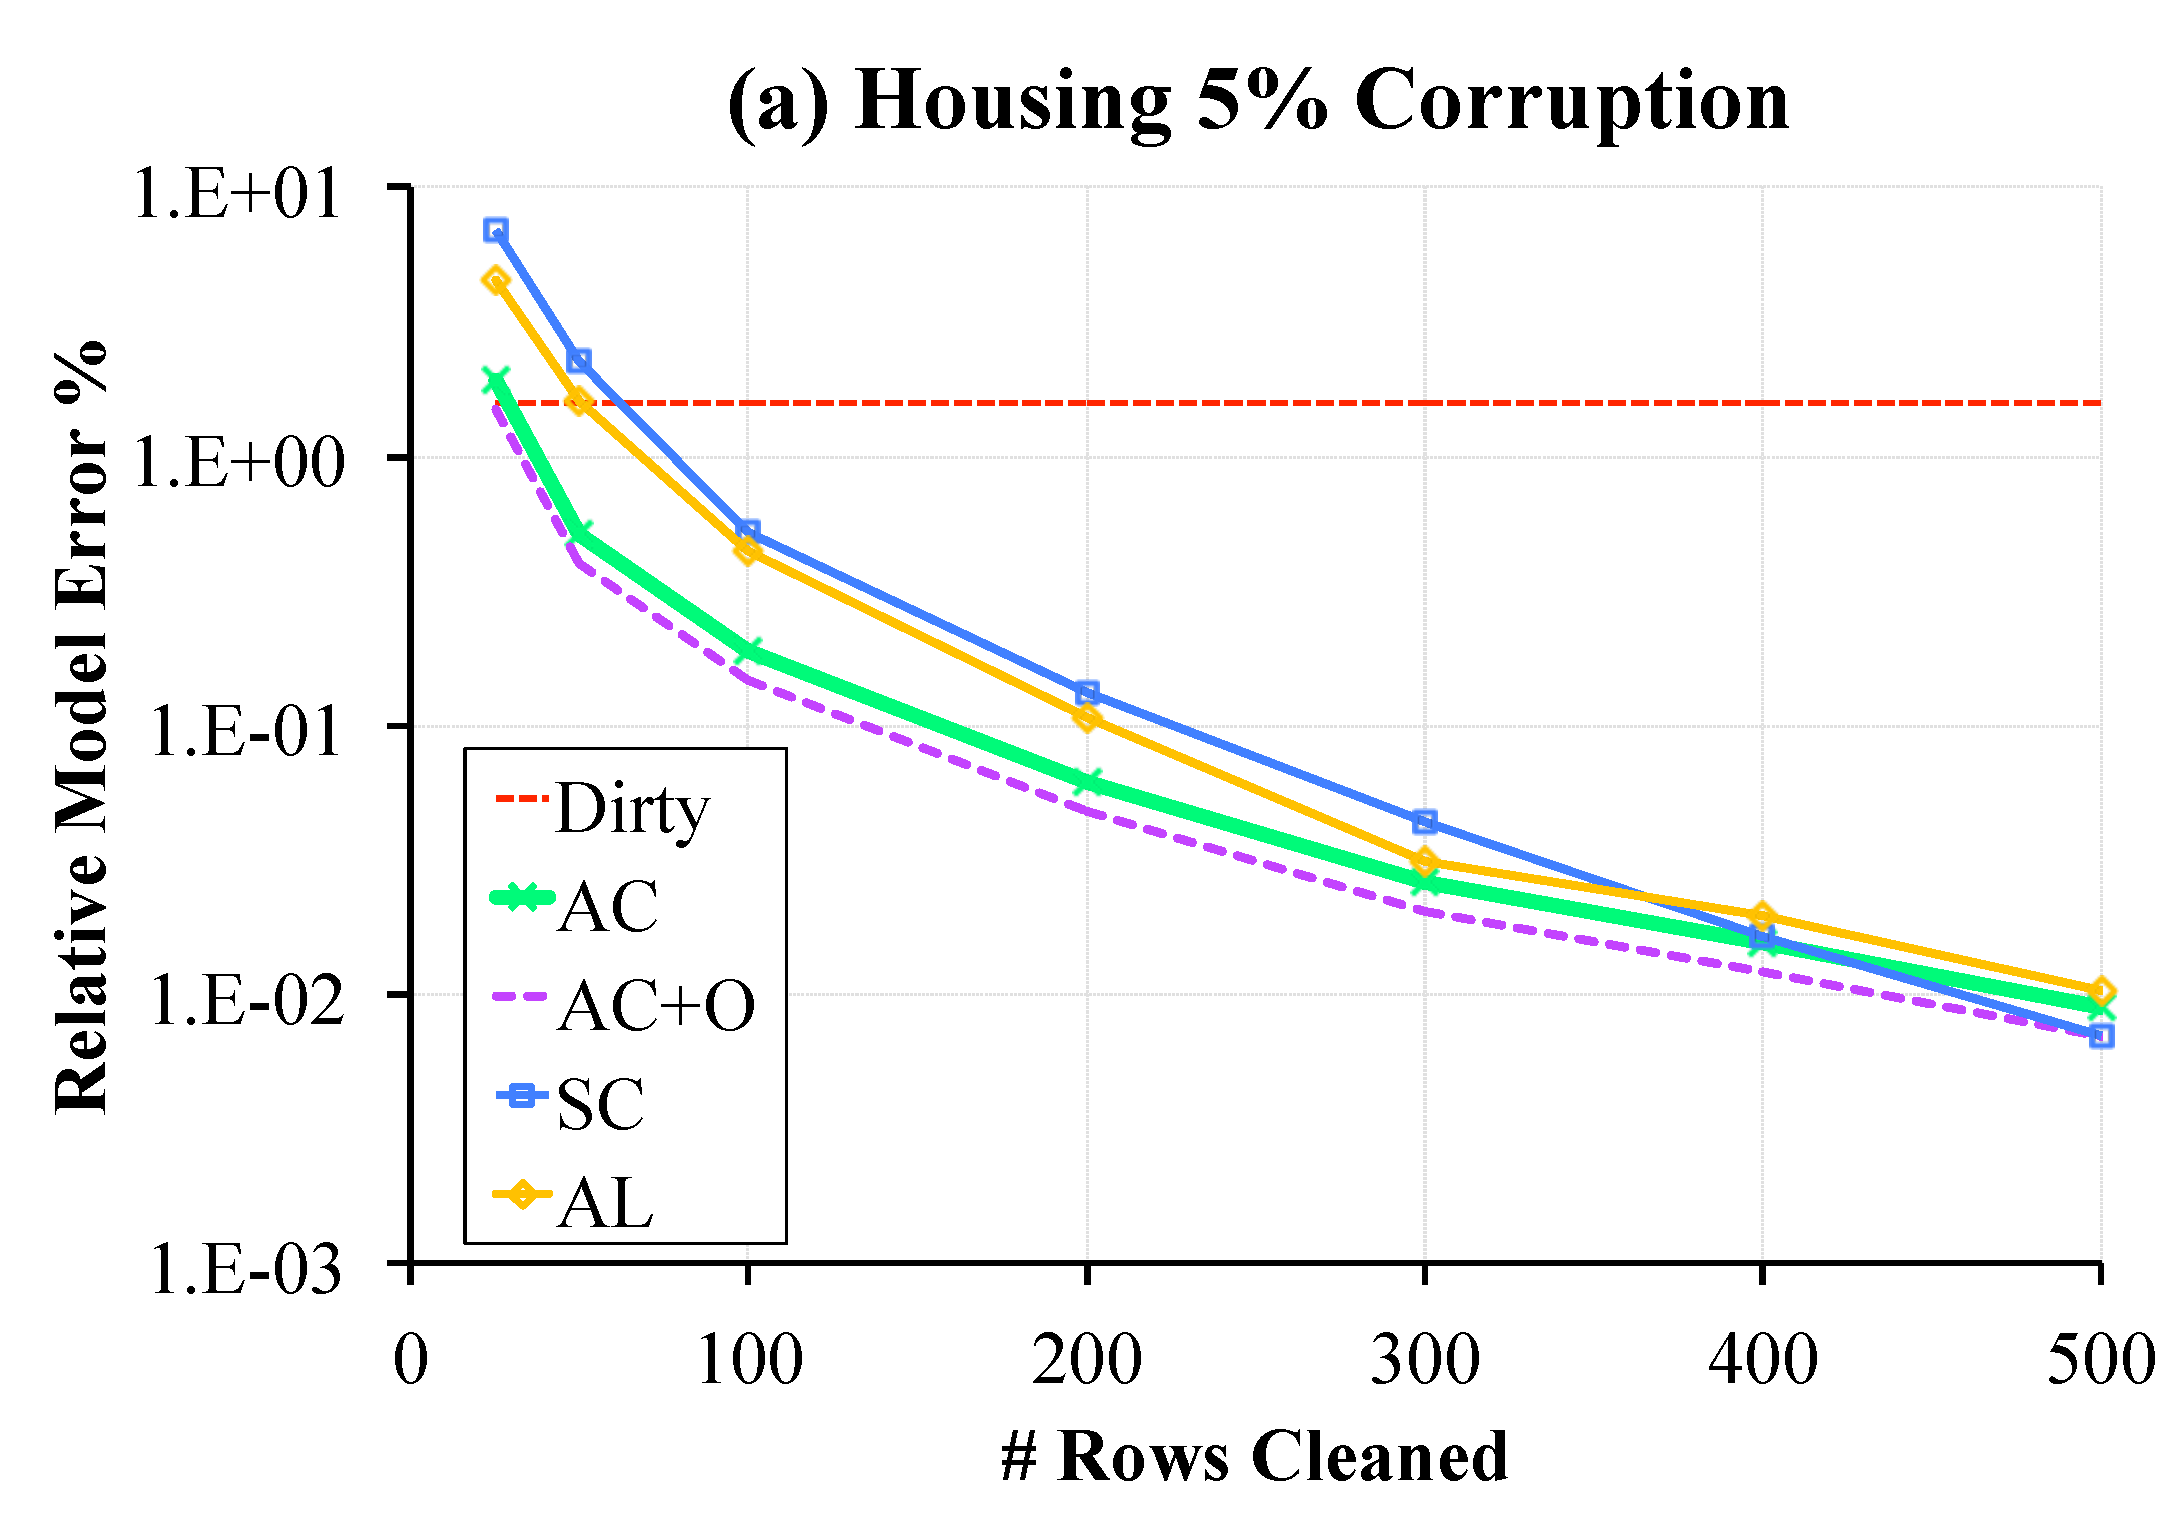
\includegraphics[scale=0.15]{exp/exp3a.pdf}
 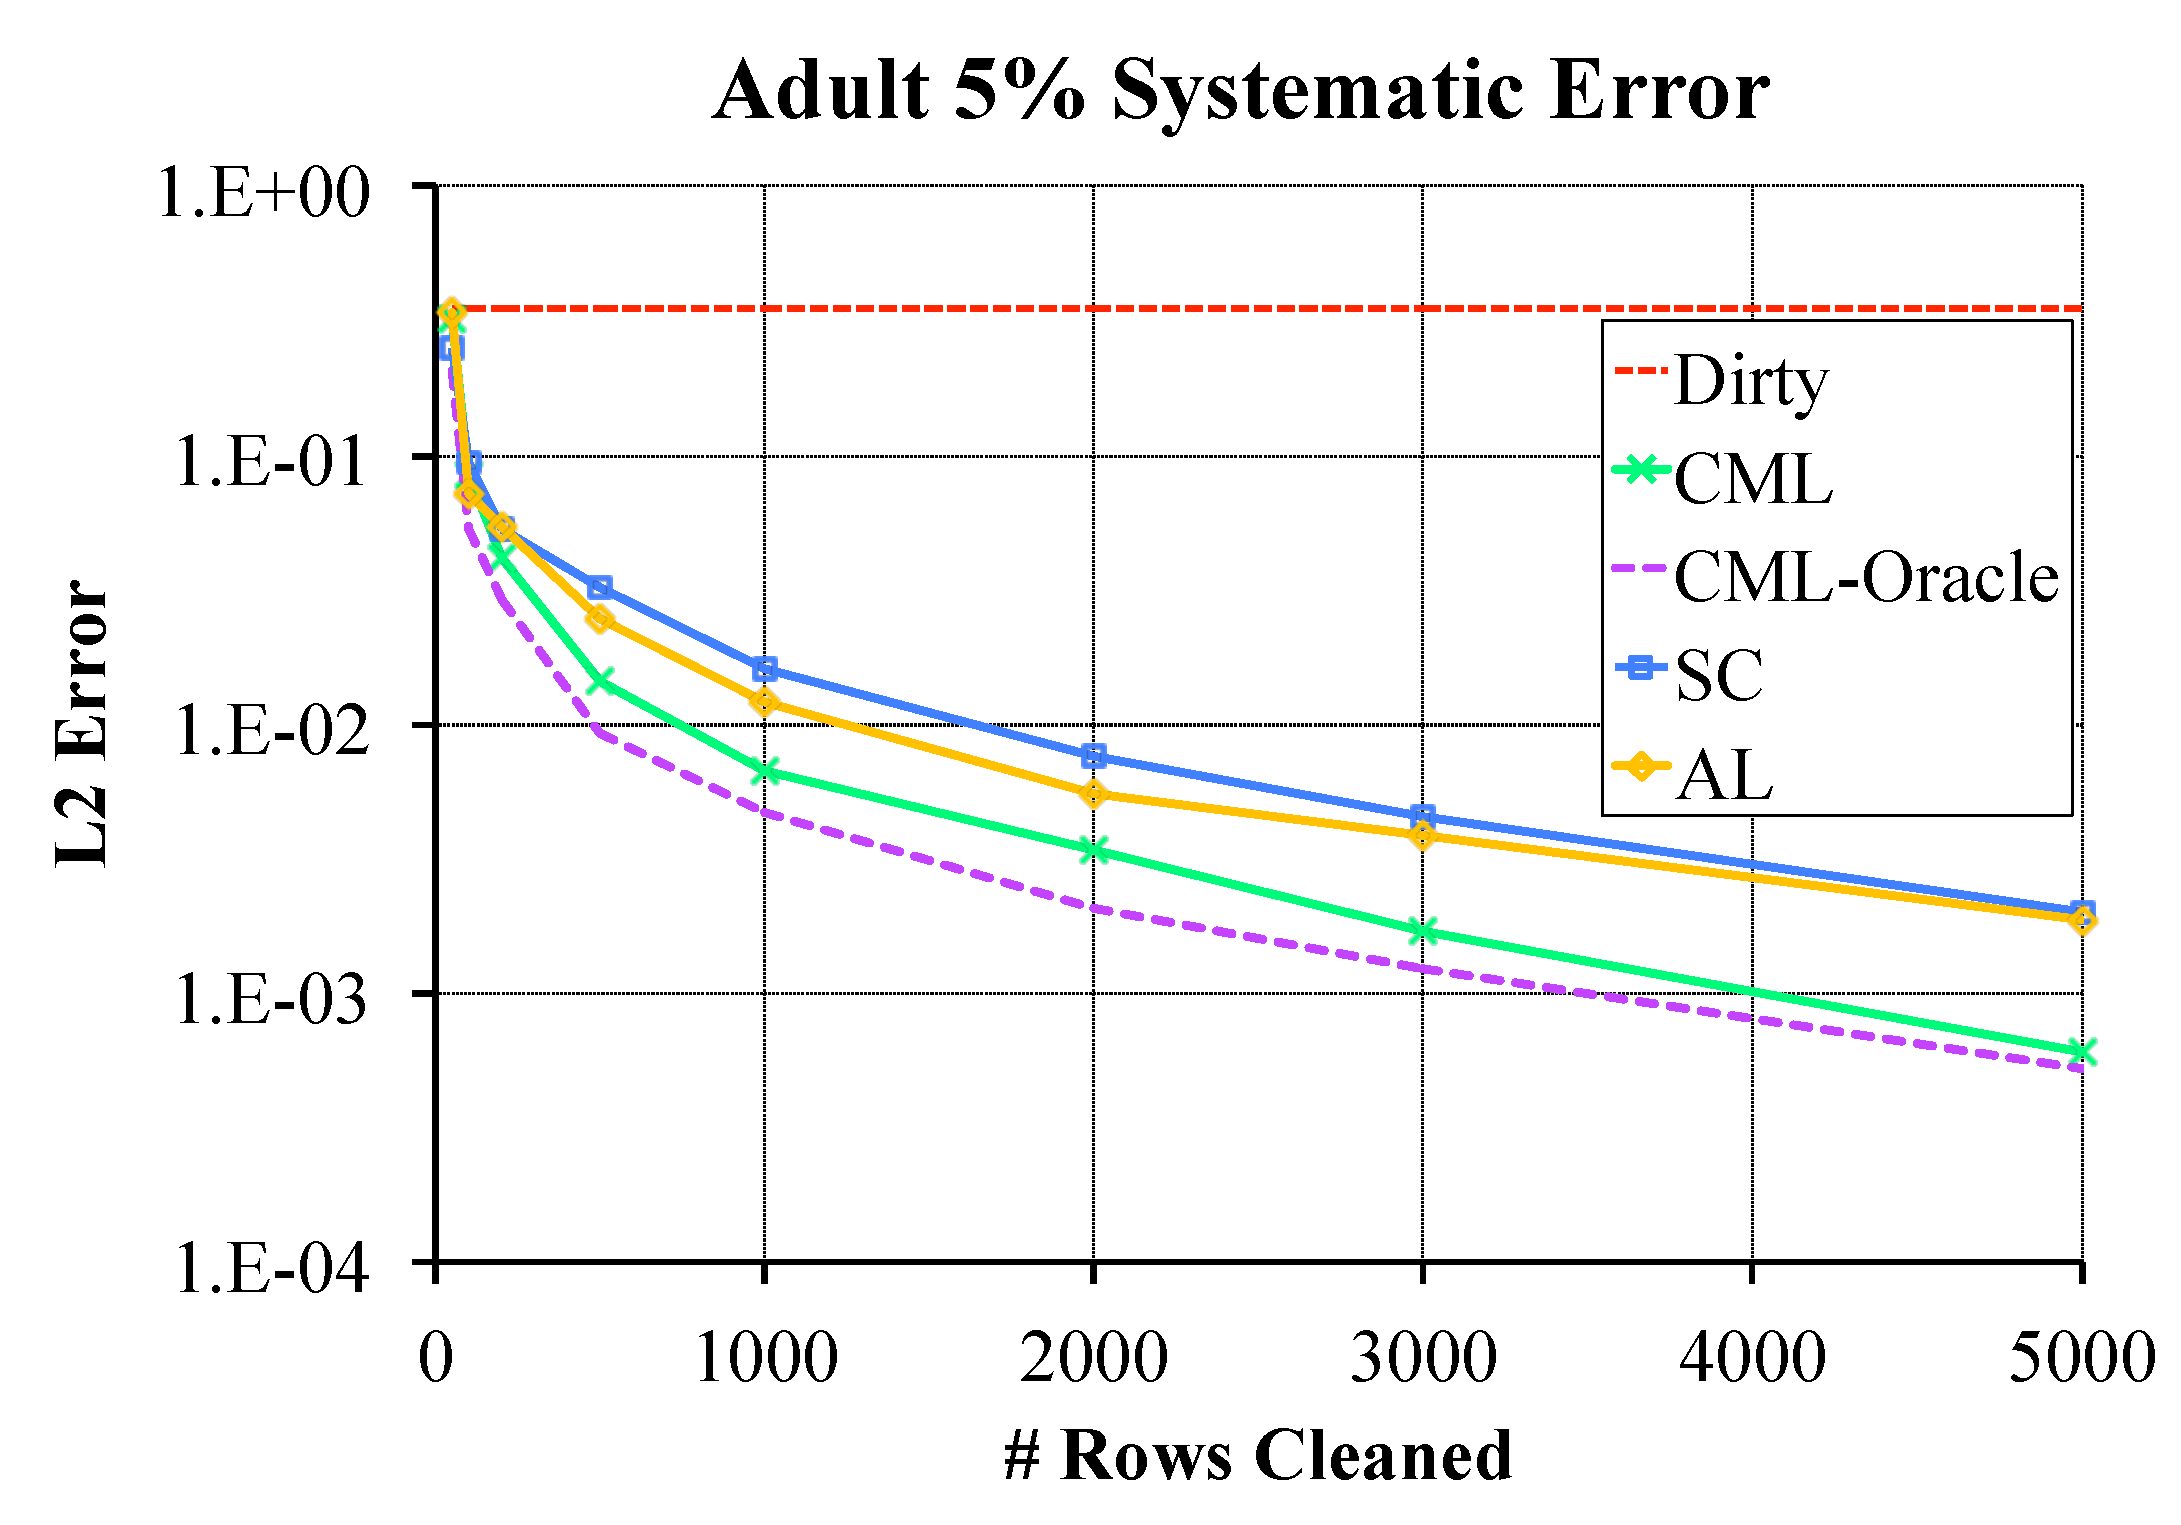
\includegraphics[scale=0.15]{exp/exp3b.pdf}
  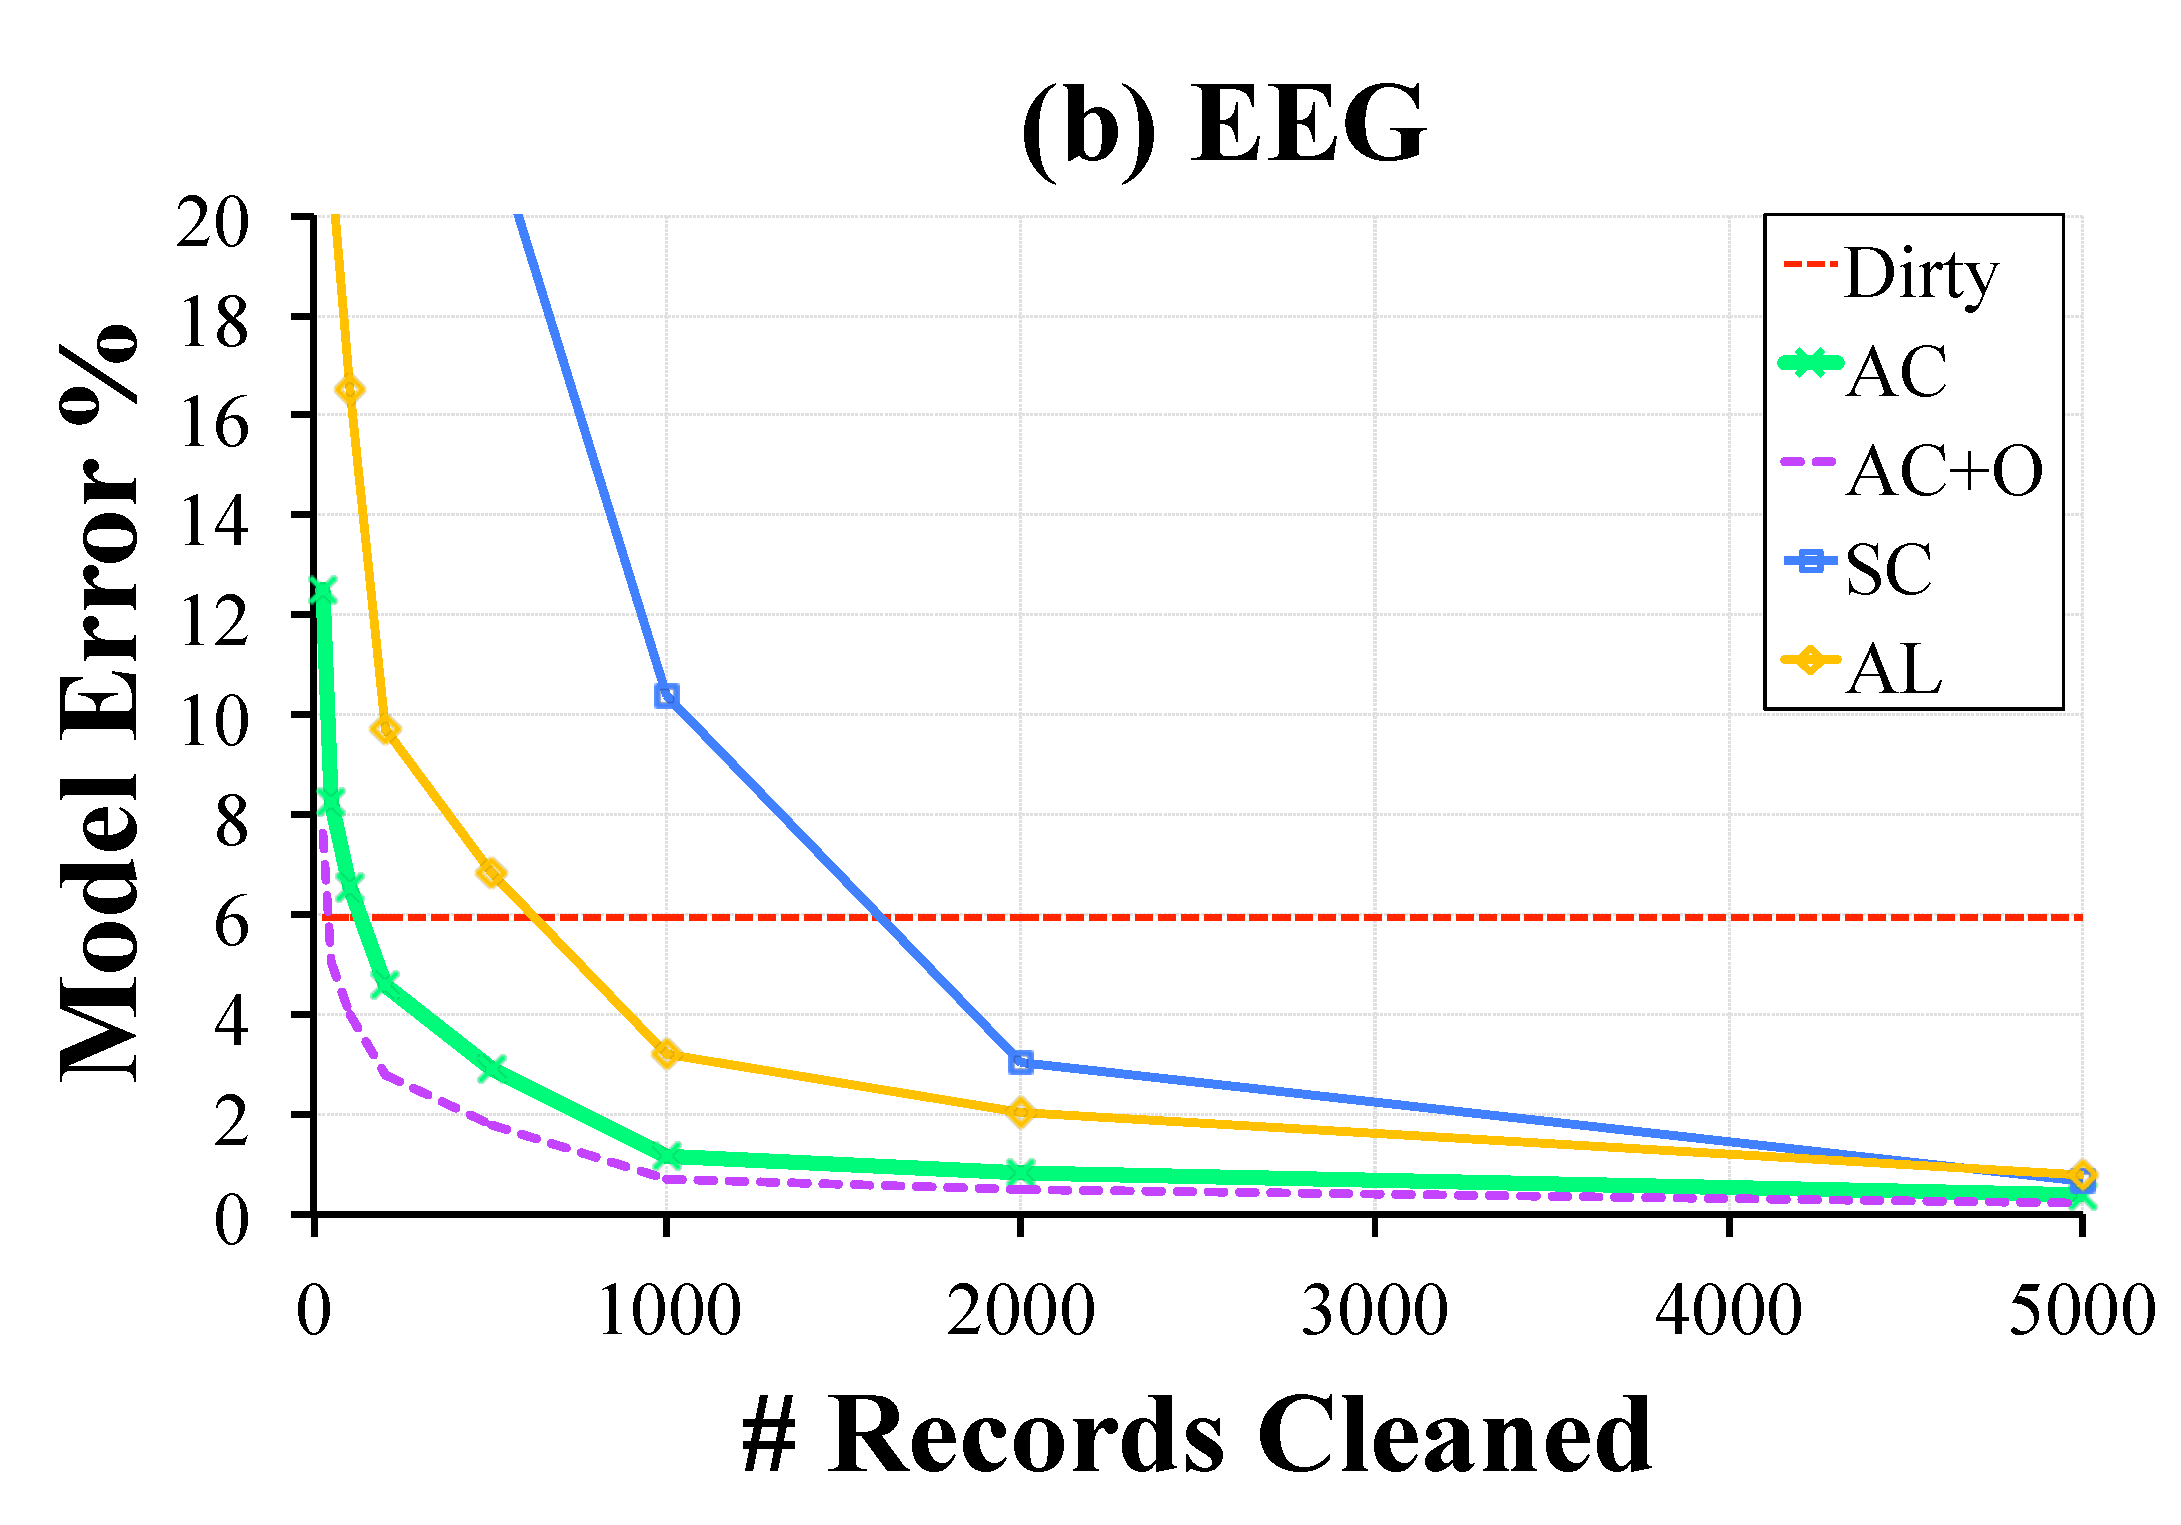
\includegraphics[scale=0.15]{exp/exp3c.pdf}
 \caption{\sys converges with a smaller sample size to the true result in comparison to Active Learning and SampleClean. \label{prio-perf}}
\end{figure*}

\subsubsection{2b. Source of Improvements}
Throughout the paper, we proposed numerous optimizations.
Now, we try to understand the source of our improvements w.r.t Active Learning and SampleClean.
We pick a single point on the curves shown in Figure \ref{prio-perf} that corresponds to 10\% of the data cleaned (55 for Housing, 4555 for Adult, 150 for EEG) and compare the performance of \sys with and without various optimizations.
We denote \sys without partitioning as (AC-P) and \sys without partitioning and importance sampling as (AC-P-I).
In Figure \ref{opts}, we plot the relative error of the alternatives w.r.t to the optimized version of \sys.
Partitioning significantly improves our results in all of the datasets, and accounts for a substantial part of the improvements over Active Learning.
However, when we remove partitioning we still see some improvements since our importance sampling relies on error impact estimates that judge how valuable a point is to the clean model rather than the dirty model in Active Learning.
Not surprisingly, when we remove both these optimizations, \sys is comparable or slightly worse than Active Learning.

\begin{figure}[ht!]
\centering
 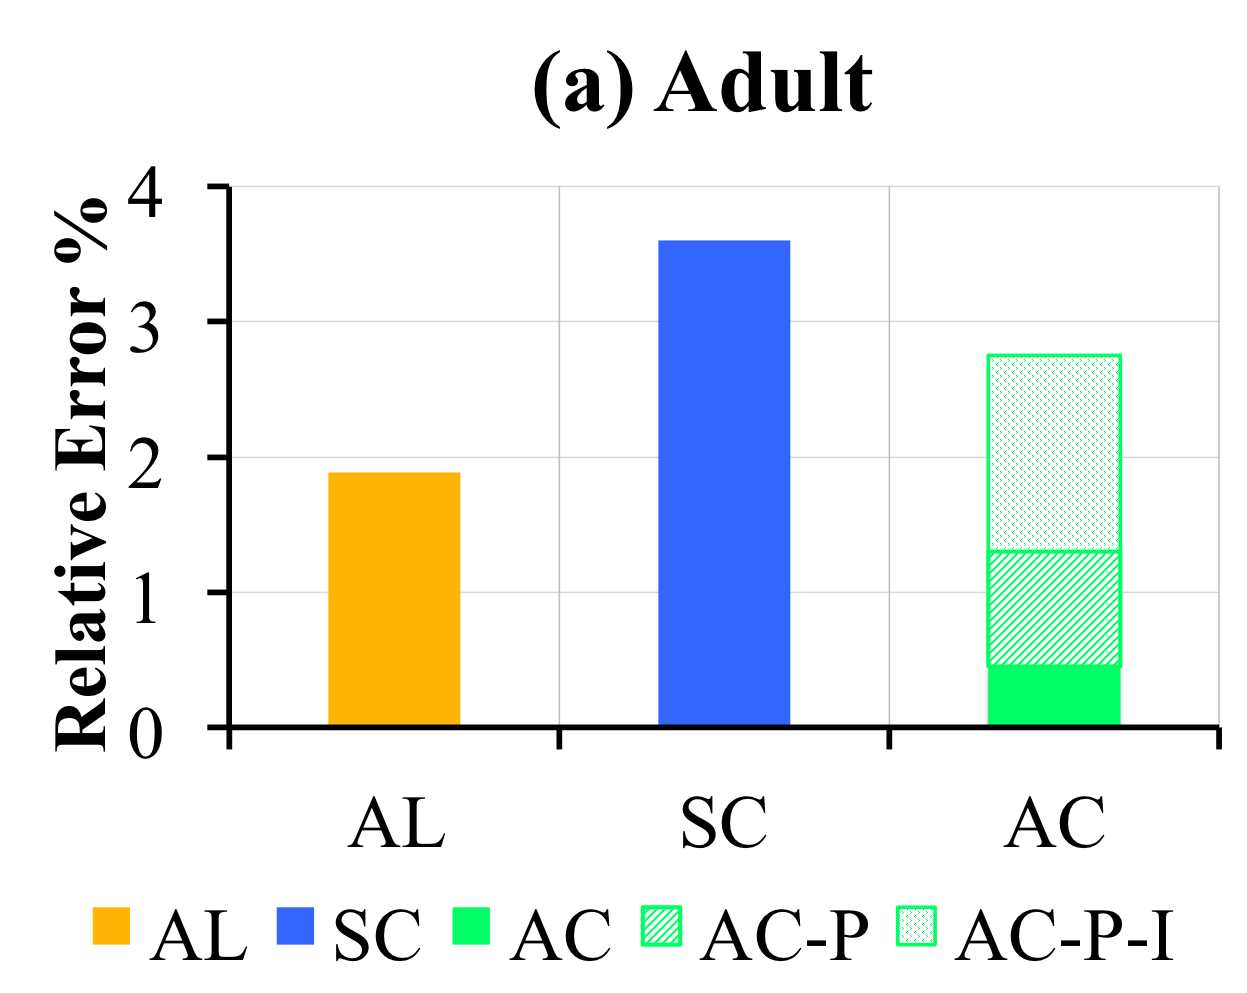
\includegraphics[width=\columnwidth]{exp/exp8.png}
 \caption{We clean 10\% of the data with the alternative algorithms and also include variants of \sys with optimization removed. We plot the relative error w.r.t the optimized \sys. Both partitioning and importance sampling lead to significant reductions in error. \label{opts}}
\end{figure}

We evalue Active Learning and \sys to better understand this relationship.
In Figure \ref{albias}, we vary the biasing effect of our random corruptions.
That is, we start with zero mean noise and increase the mean value and variance of the noise.
Since Active Learning uses the gradient, if there is zero mean noise, in expectation, the dirty data and clean data are the same.
However, as the bias increases, the fact that Active Learning prioritizes w.r.t to the dirty data matters more and becomes increasingly erroneous w.r.t to \sys.

\begin{figure}[ht!]
\centering
 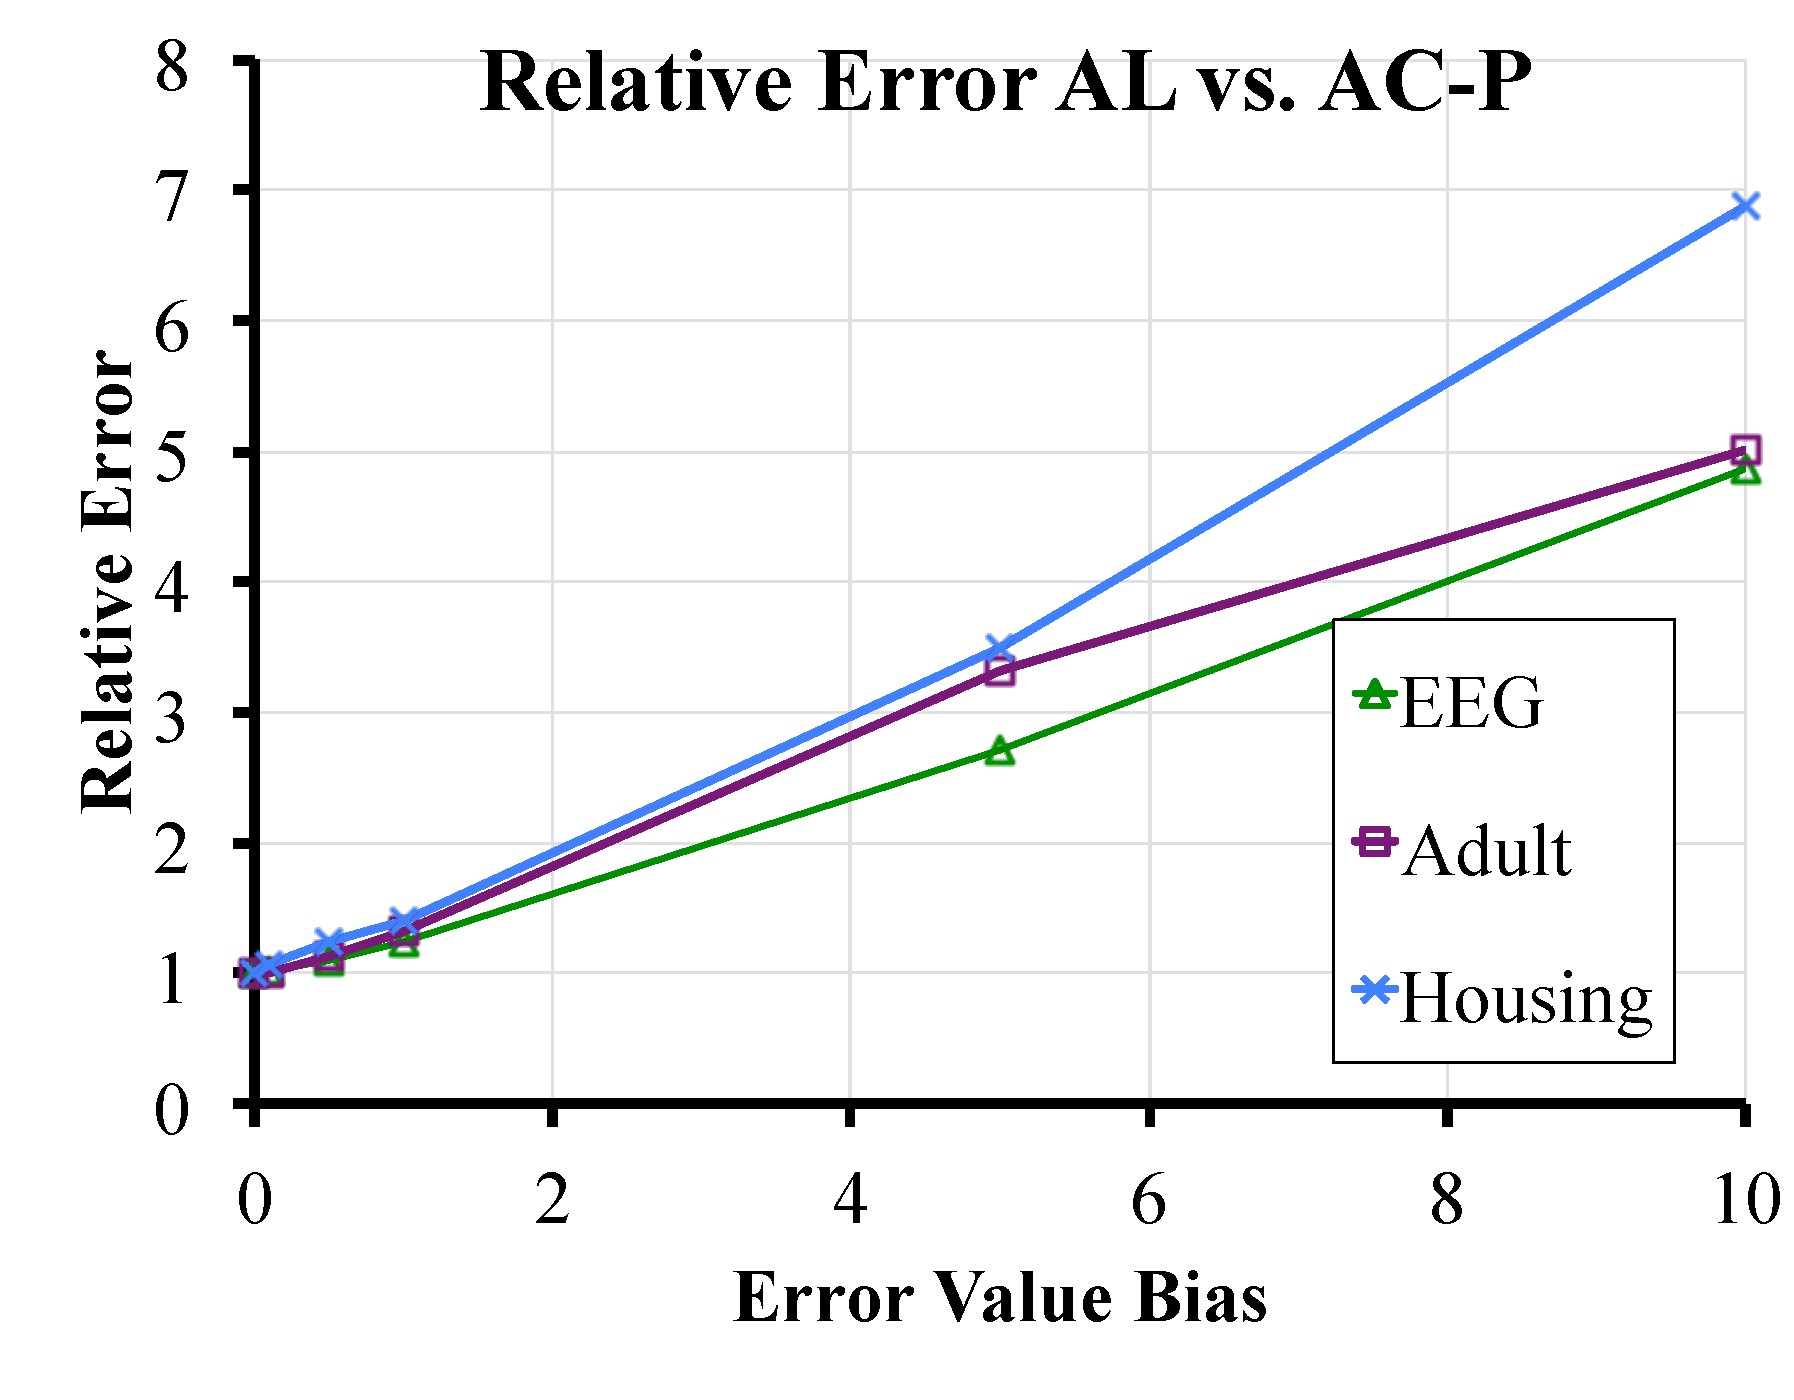
\includegraphics[width=0.6\columnwidth]{exp/exp10.pdf}
 \caption{As we increase the biasing nature of the corruption, Active Learning is increasingly erroneous w.r.t \sys. \label{albias}}
\end{figure}

\subsubsection{2c. Error Dependence}
Both Active Learning and \sys outperform SampleClean in our experiments.
In our next experiment, we try to understand how much of this performance 
is due to the initialization (i.e., SampleClean trains a model from ``scratch").
We vary the rate of random error, thus making the initialization more and more arbitrary, 
and measure the relative performance between SampleClean and \sys.
Since SampleClean only acts on a clean sample of data, it is robust to data error.
So at some point, the errors in the data are so significant that training a model on a small but clean sample of data is more efficient than iteratively updating the dirty model.

In Figure \ref{bias}, we present the results from this experiment.
We corrupt entries from the data matrix of the Adult dataset at random (probability on plotted on the x-axis).
Then, we measure the number of records we need to clean before we have a relative error of 0.1\%.
We find that at about 30\% corruption rate, SampleClean is more accurate than \sys.
Since the Adult dataset has 12 features, a 30\% corruption rate corresponds to each example with 3.6 features incorrect on average.
We optimized \sys for sparse and relatively small errors but it still shows reasonable performance even in this highly erroneous setting. 
At higher corruption rates, \sys requires more than one epoch to converge to an accurate answer which requires cleaning almost all of the data.

\begin{figure}[ht!]
\centering
 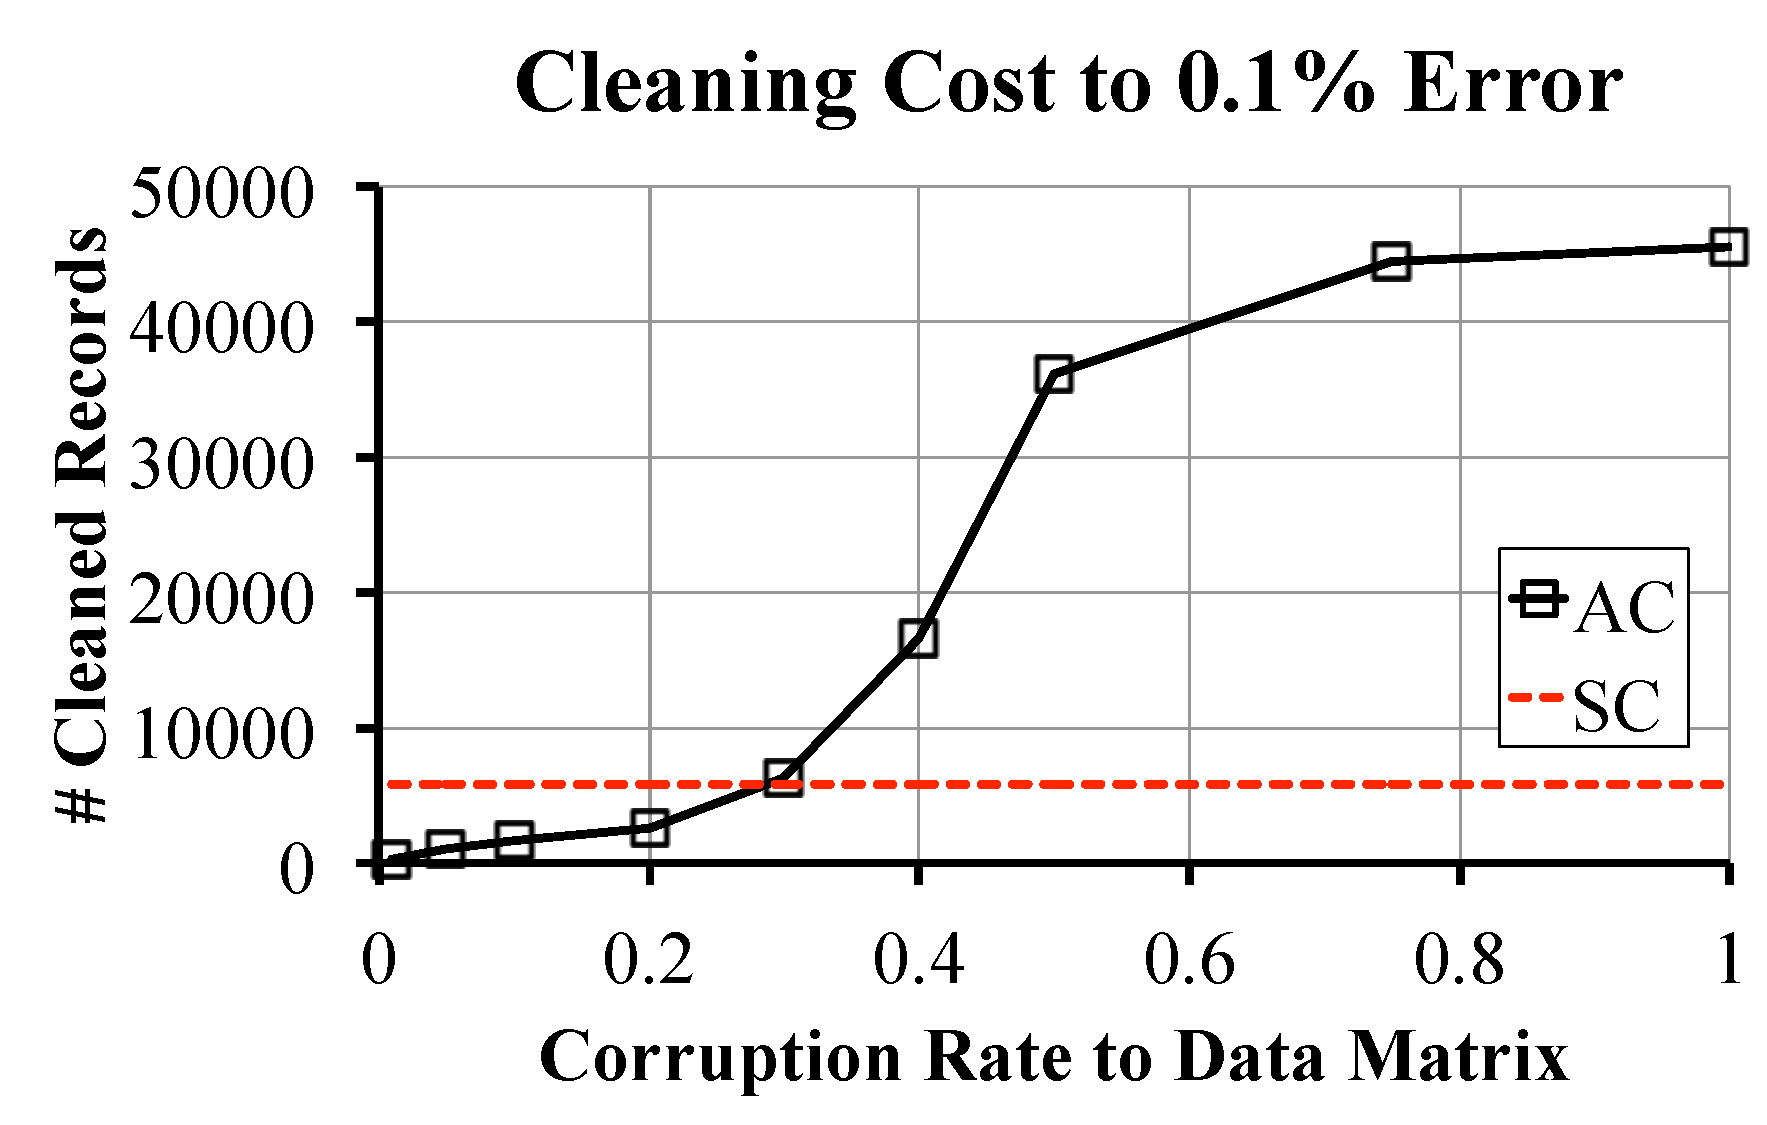
\includegraphics[width=0.6\columnwidth]{exp/exp9.pdf}
 \caption{We corrupt an increasing number of entries in the data matrix. At about 30\% corrupted, \sys is no longer more efficient than SampleClean. \label{bias}}
\end{figure}

\subsubsection{2d. Testing Accuracy}
In the previous experiments, we studied the relative model error which measures the training loss. 
However, to an end user the metric that matters is test accuracy.
In the next experiment, we try to understand how reductions in model error correlate to improvements in test error.
In Figure \ref{prio-tperf}, we present the results for the three datasets: Adult, Housing, and EEG.
We find that in two of the datasets, Housing and Adult, \sys converges to clean test accuracy faster than the alternatives.

However, there is a curious negative result with the EEG dataset that we would like to highlight. 
We find that even though \sys has significantly lower model error (Figure \ref{prio-perf}), this does not correspond to as significant of an increase in test accuracy.
We speculate this is due to the inherrent hardness of the EEG classification problem.
\sys may encourage overfitting at intermediate results for hard classification tasks.
The solution to this problem may be to add additional regularization, thus actually changing the optimization problem.
We hope to explore this problem in further detail in future work.

\begin{figure*}[t]
\centering
 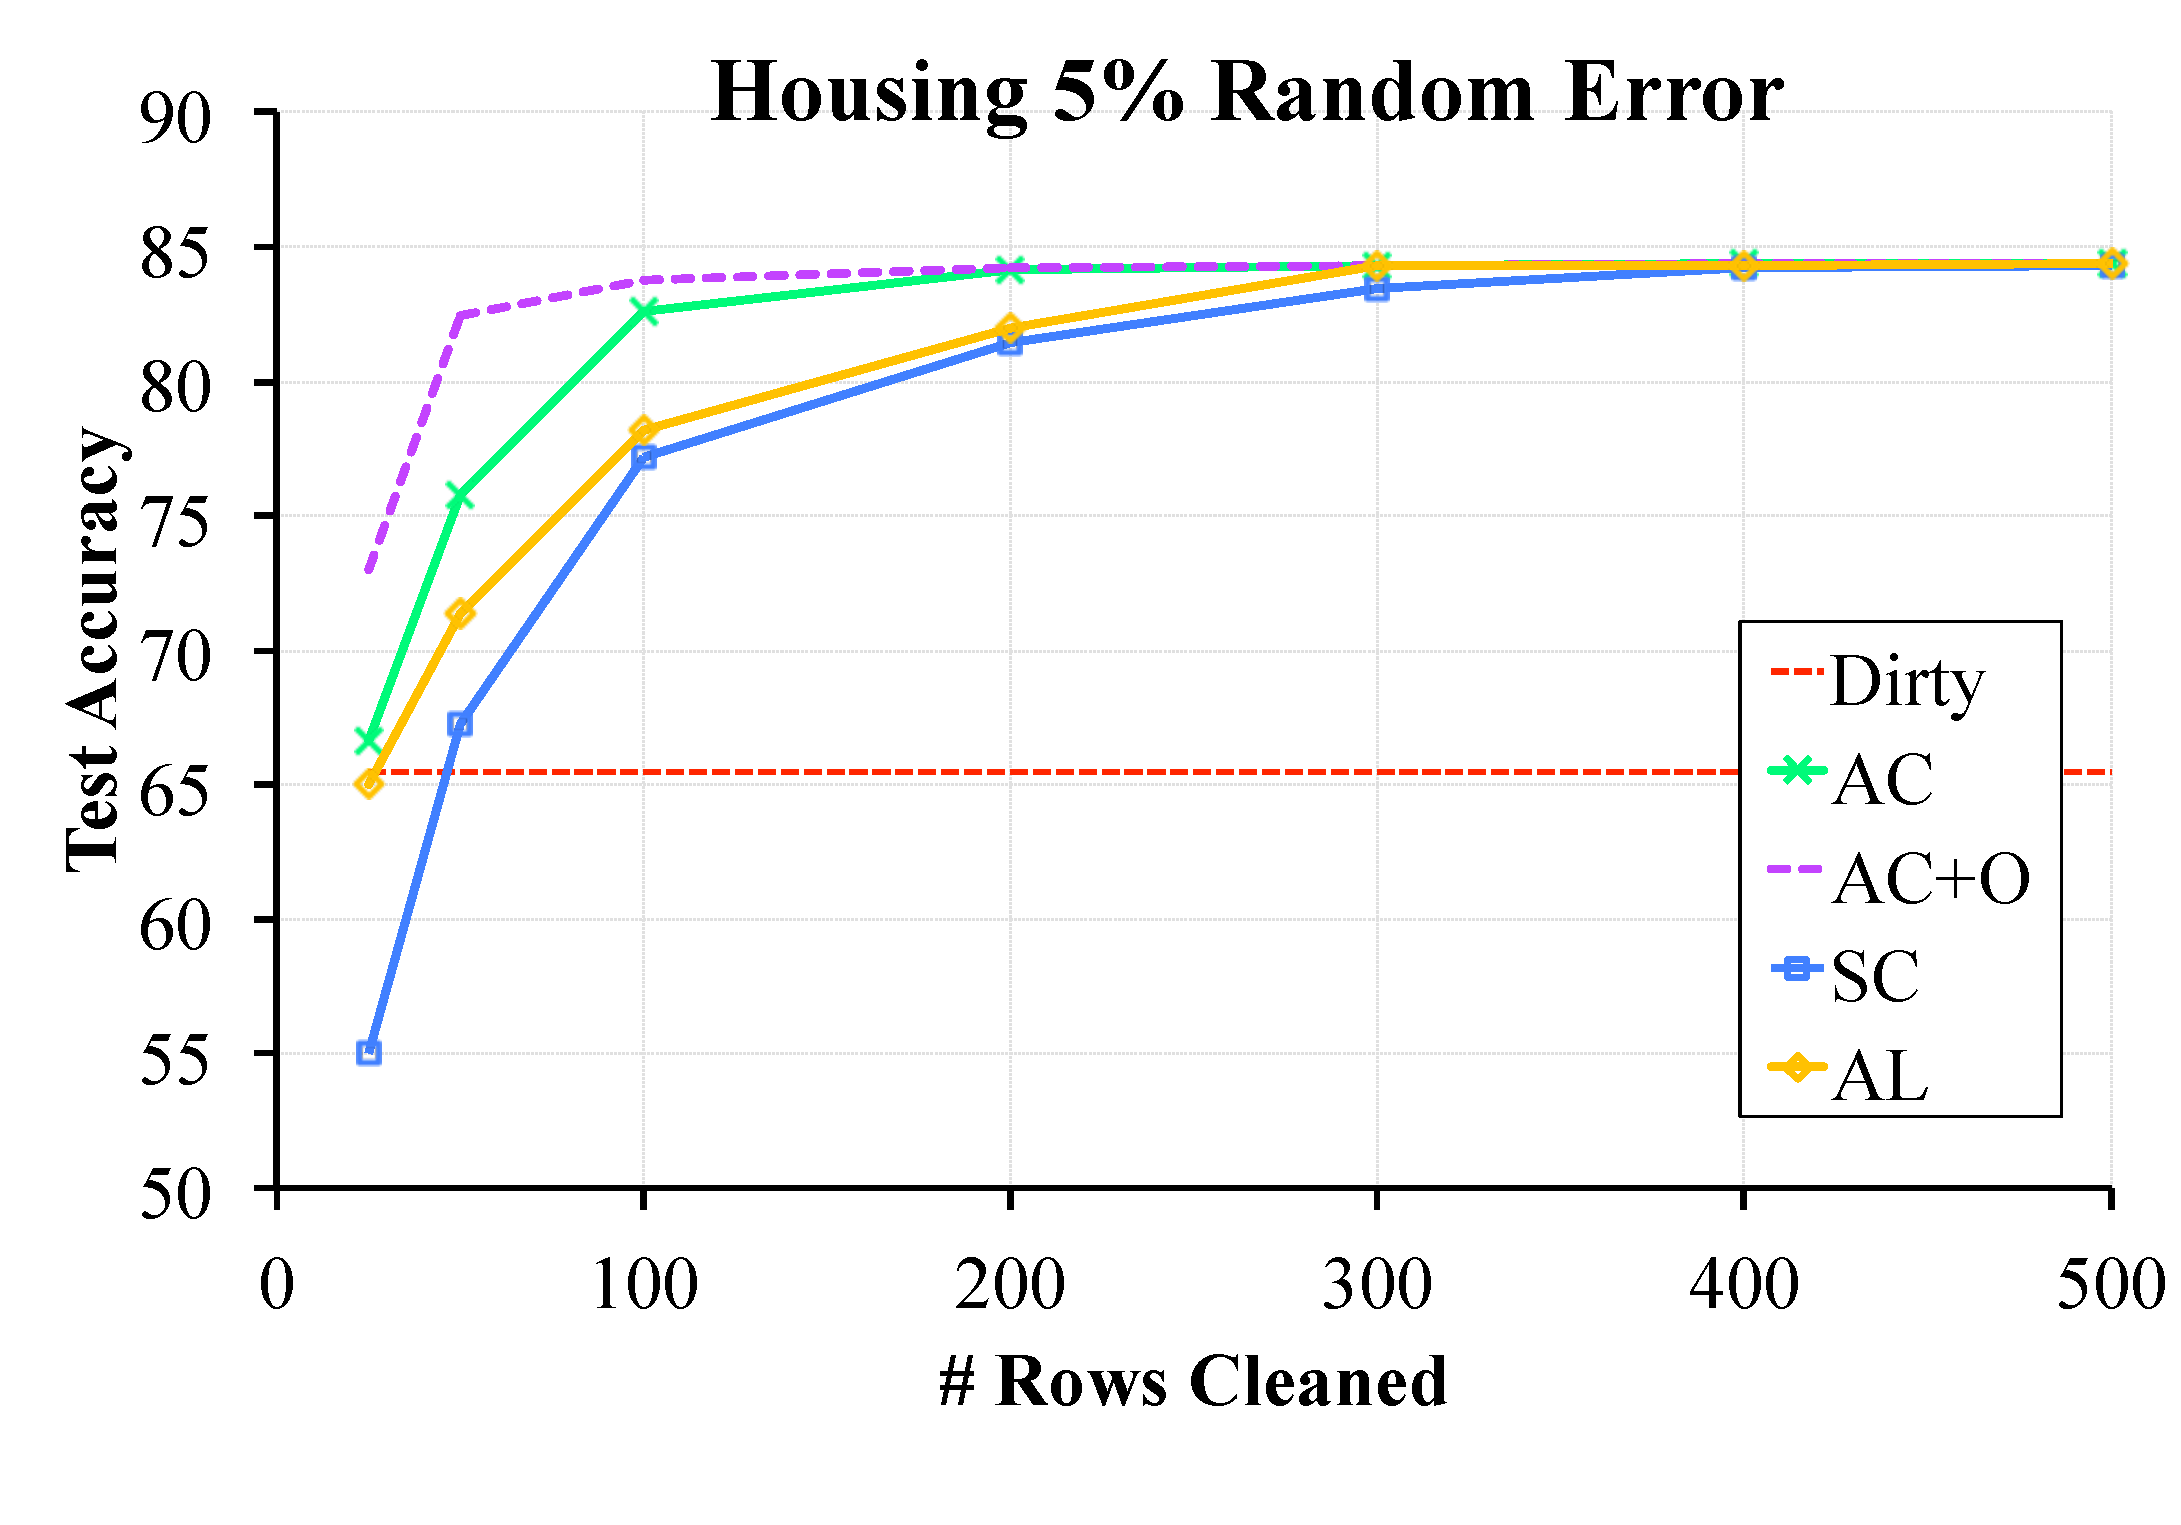
\includegraphics[scale=0.15]{exp/exp3aa.pdf}
 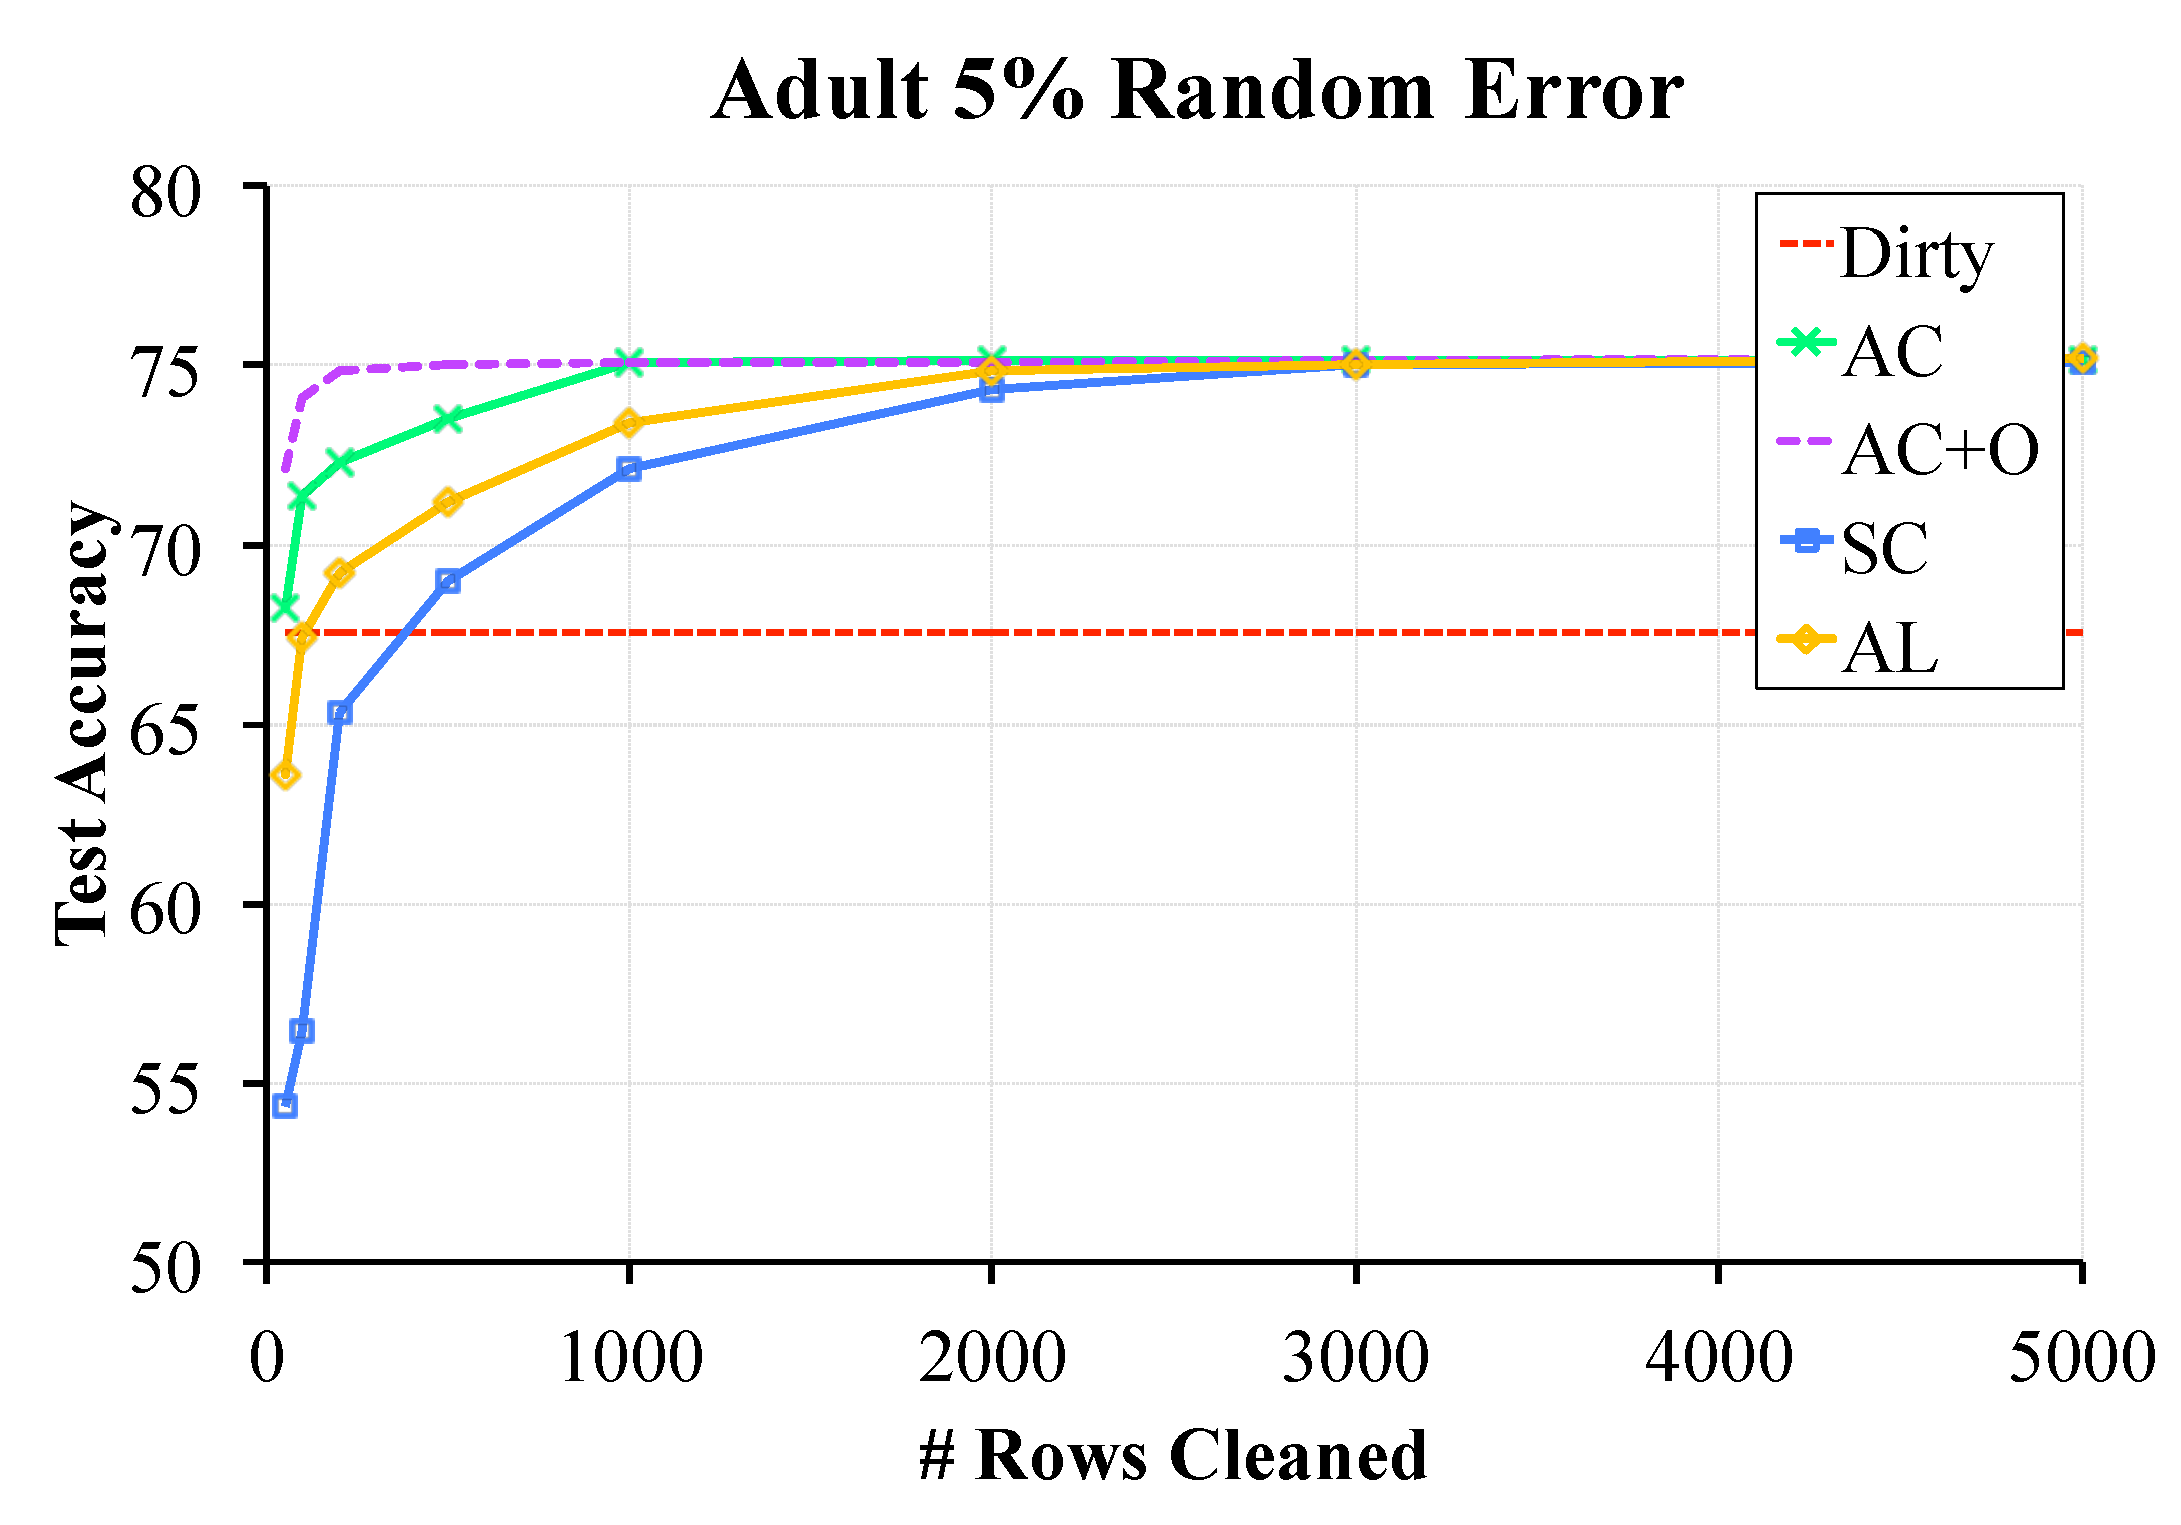
\includegraphics[scale=0.15]{exp/exp3bb.pdf}
  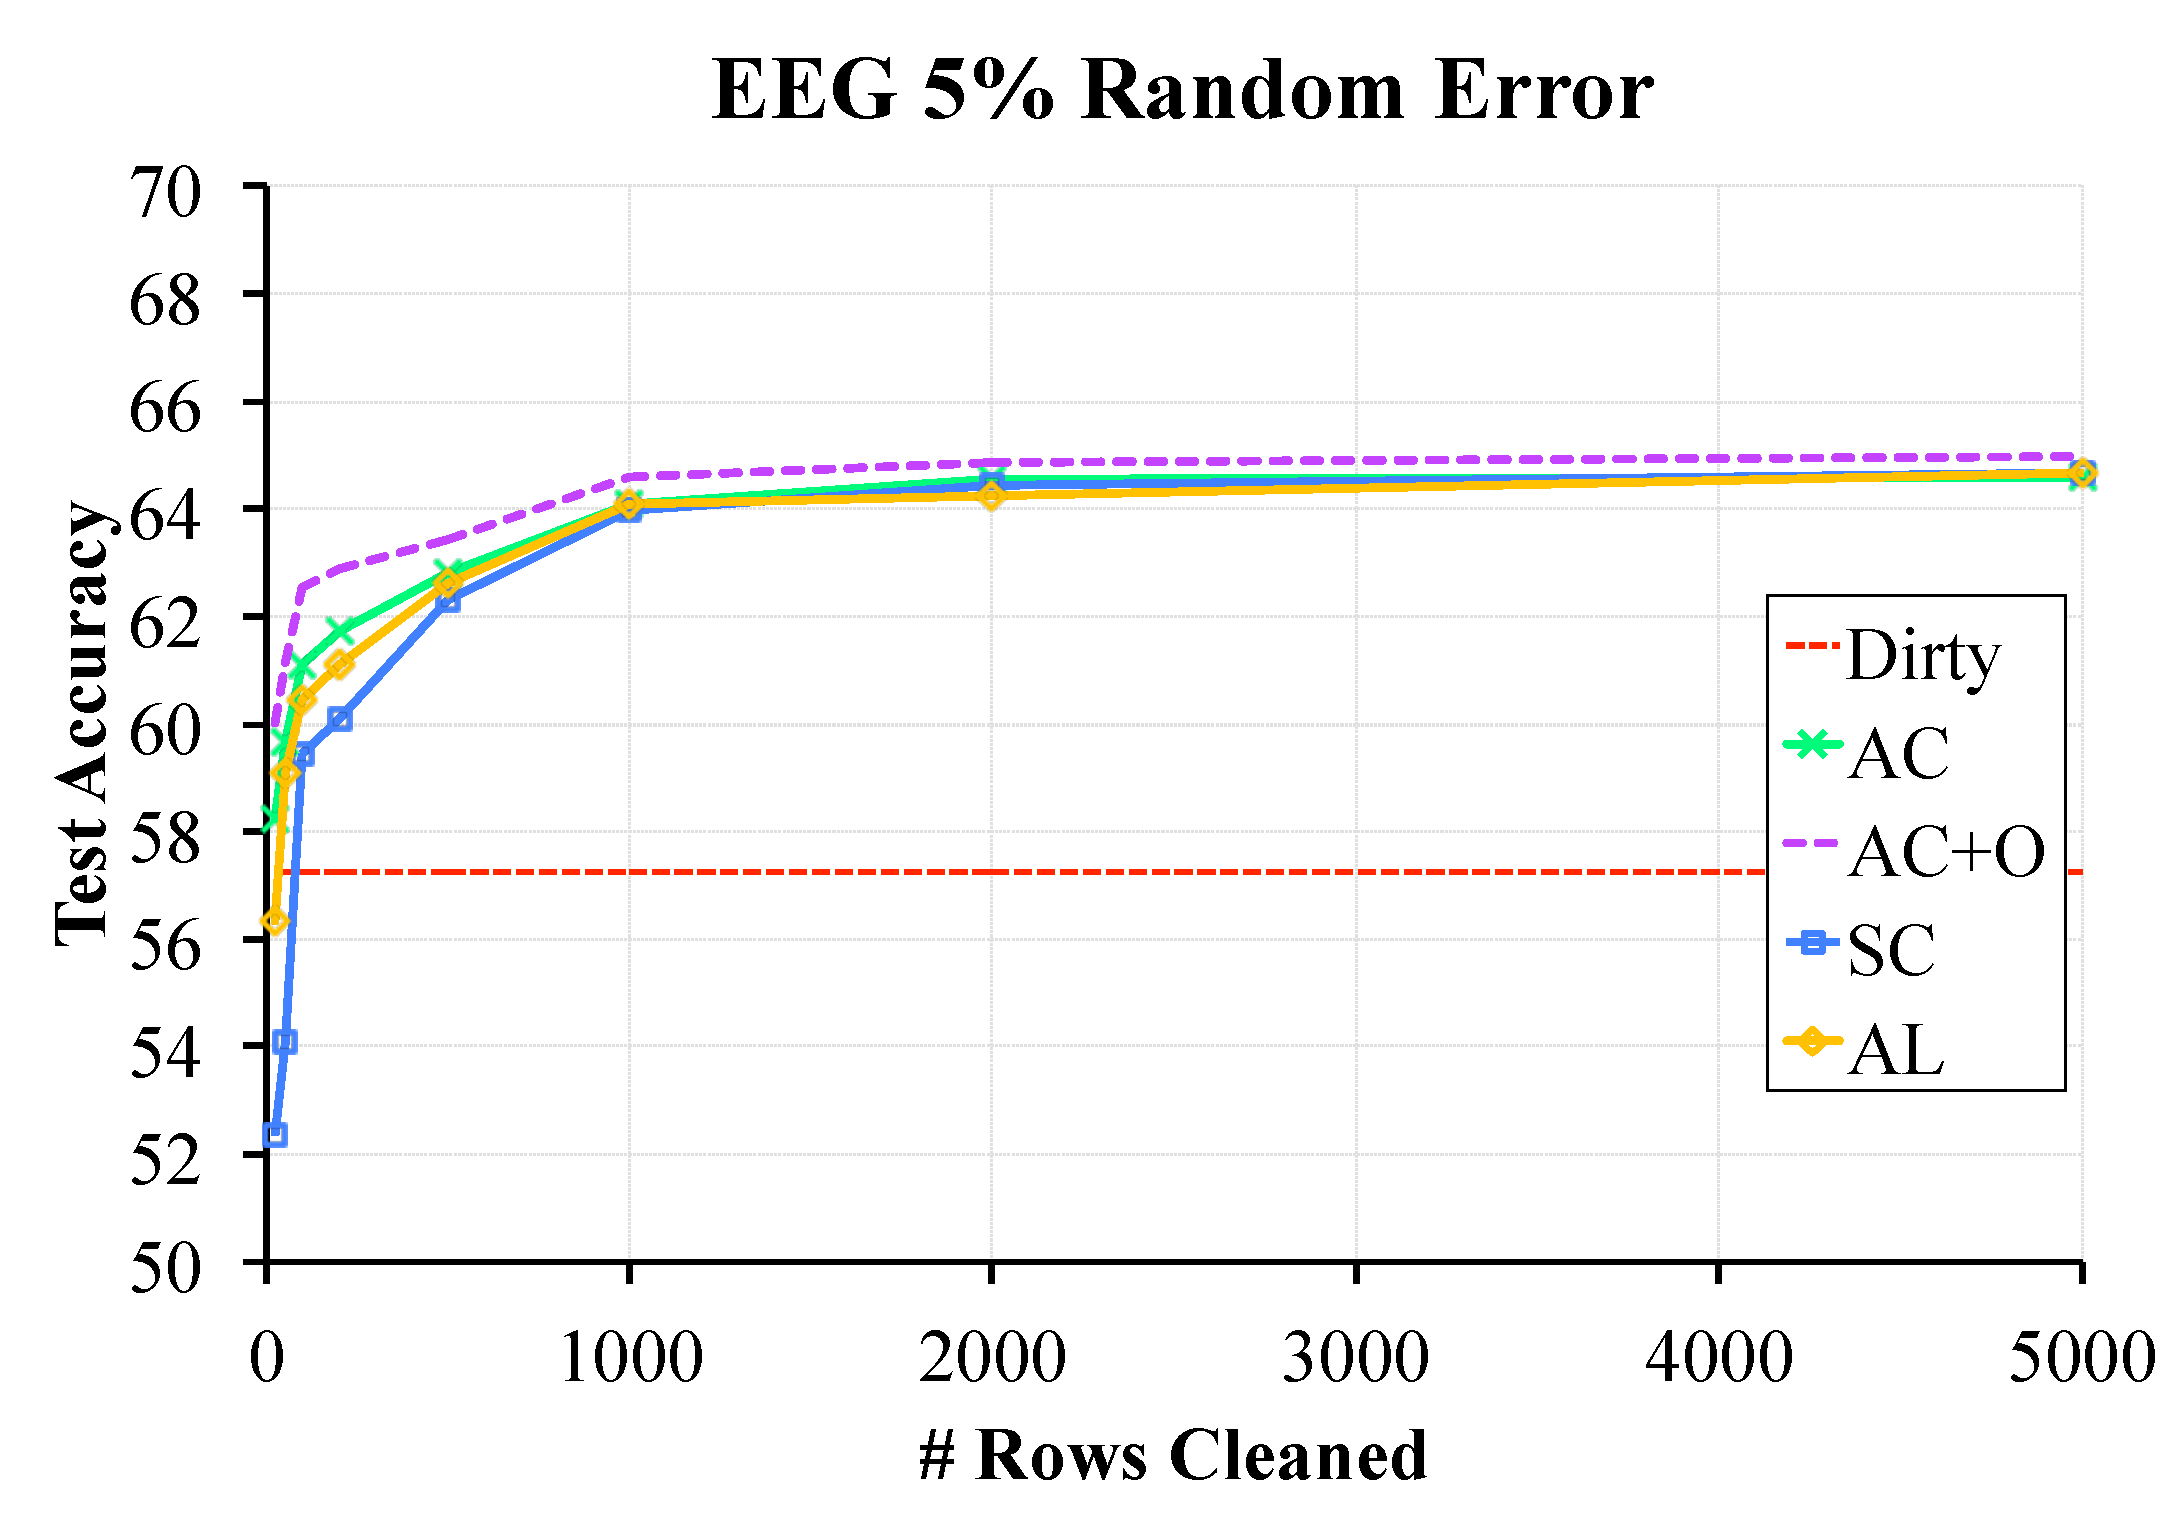
\includegraphics[scale=0.15]{exp/exp3cc.pdf}
 \caption{\sys converges with a smaller sample size to the maximum test accuracy in comparison to Active Learning and SampleClean. \label{prio-tperf}}
\end{figure*}

\subsection{Experiment 3. Predicates vs. Classification}

\subsubsection{3a. Basic Performance}
In the next set of experiments, we explore the error partitioning in more detail.
We presented two models for error sampling, one where we are given a set of candidate dirty records through a predicate and one where we have to learn this predicate as we clean.
In Figure \ref{pred-perf}, we overlay the convergence plots in the previous experiments with a curve (denoted by AC+C) that represents \sys using a classifier instead of an error predicate.
We use an SVM classifier to predict errors.
We find an interesting tradeoff where initially \sys is comparable to Active Learning (explanation for why seen in Figure \ref{opts}), as our classifier becomes more effective the partitioning improves the performance.

\begin{figure}[t]
\centering
 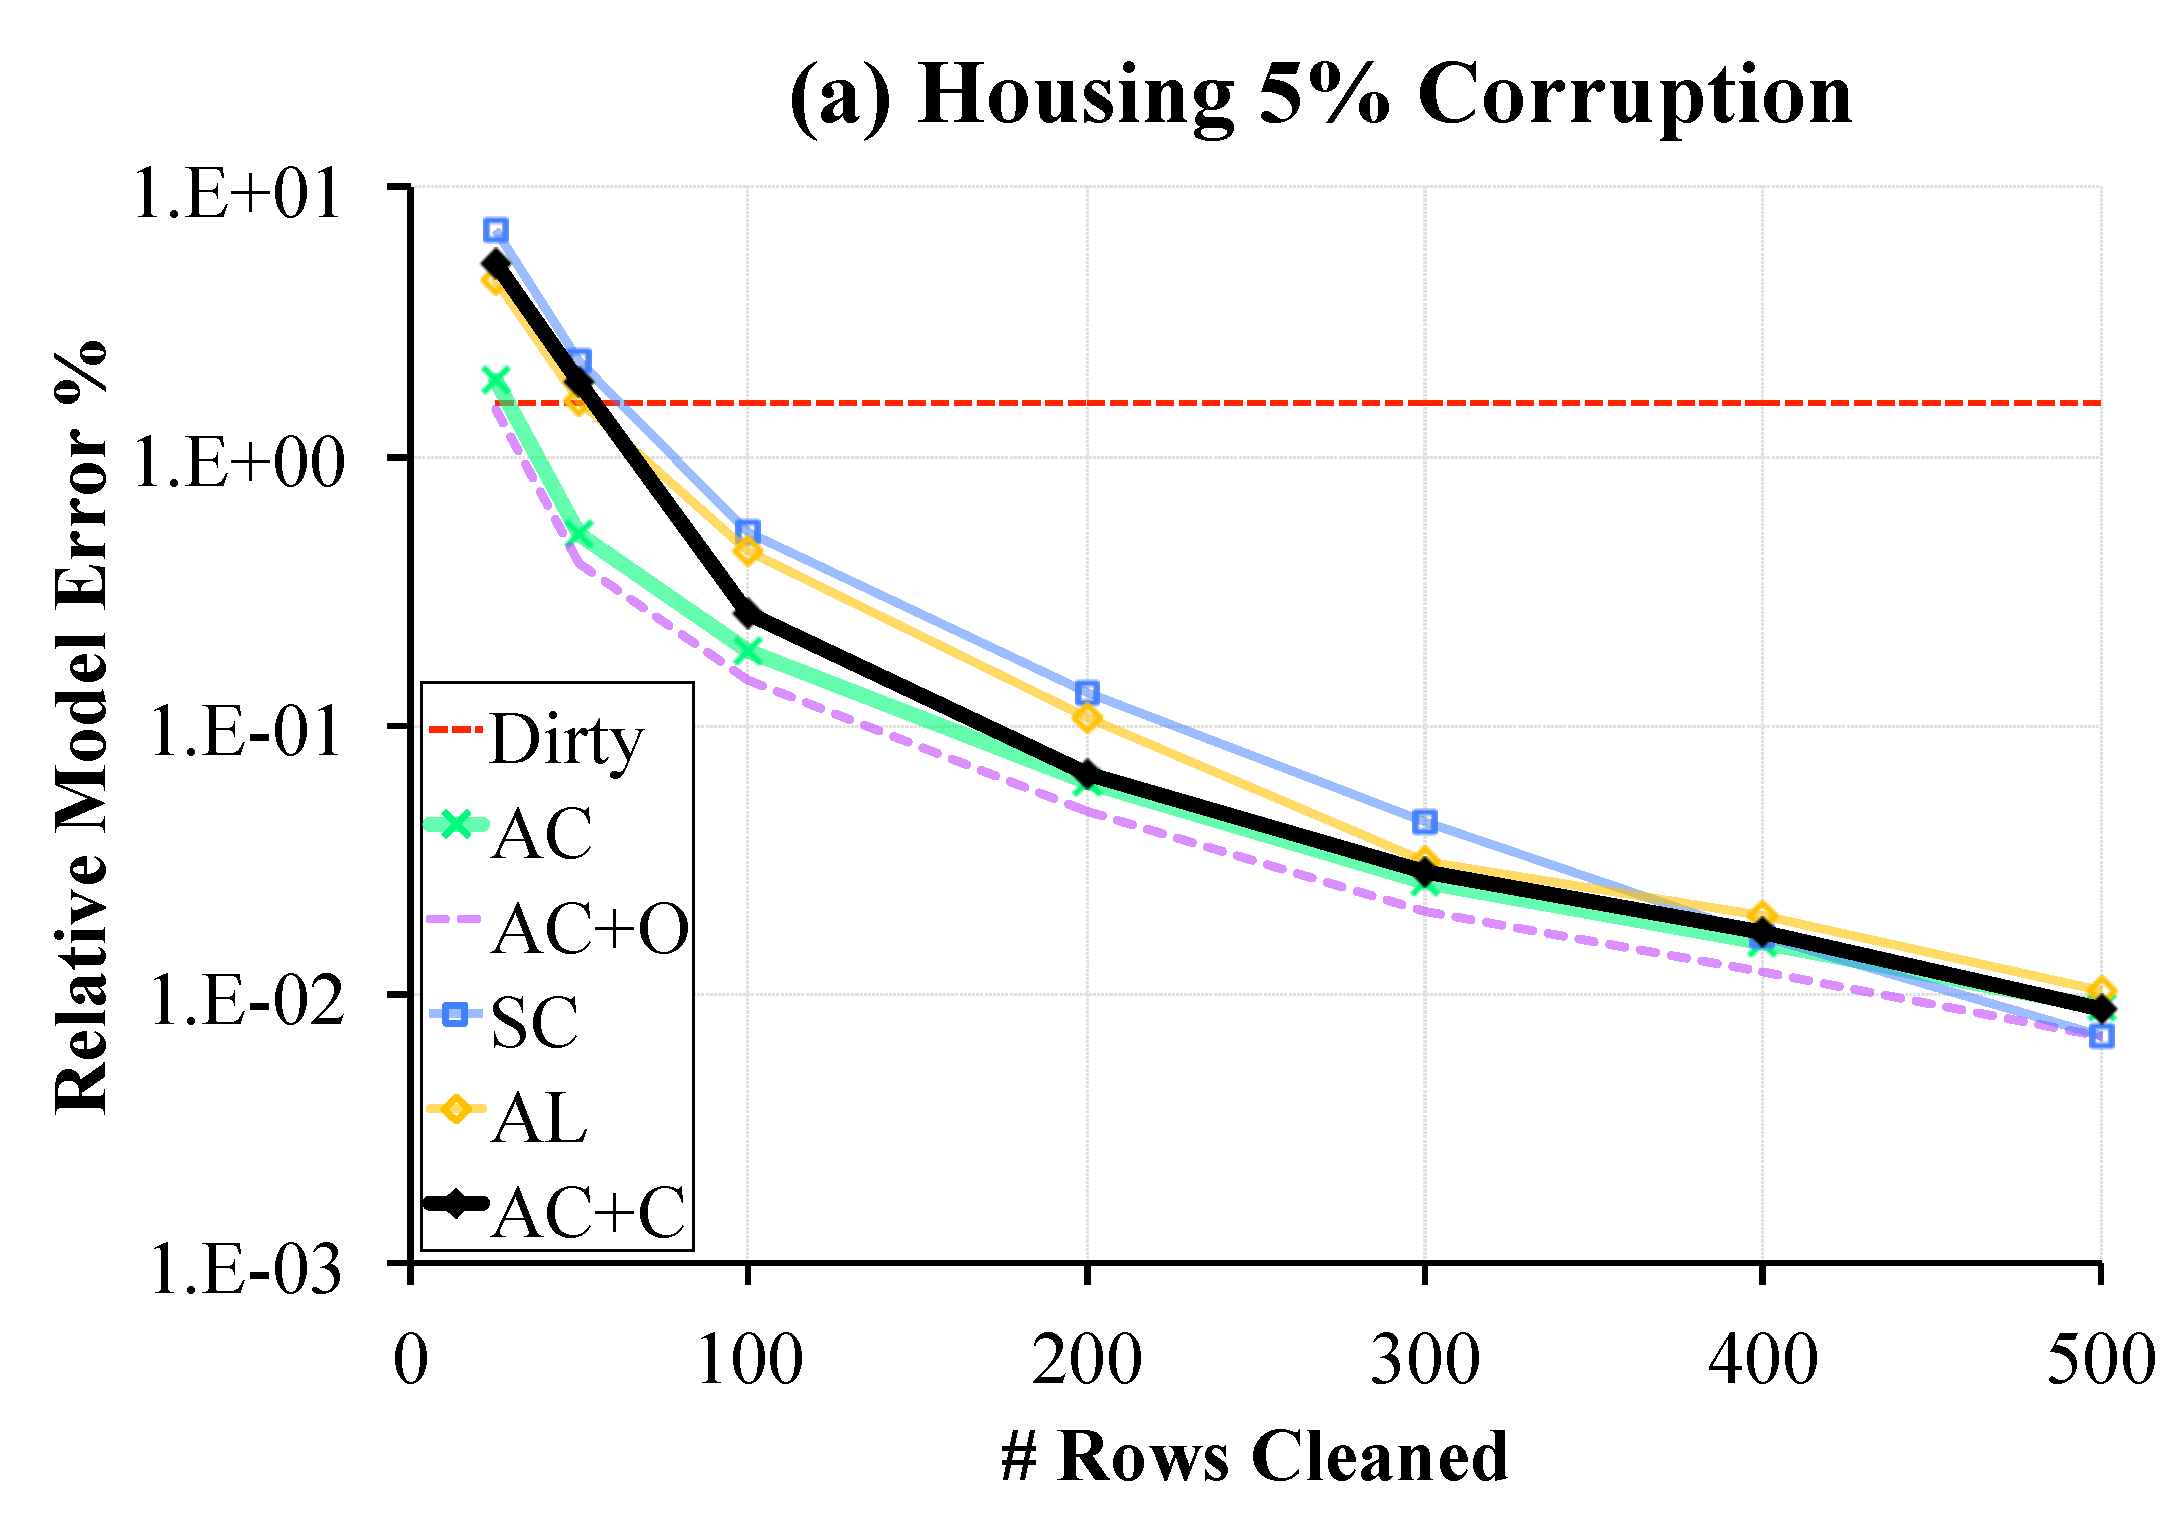
\includegraphics[width=0.48\columnwidth]{exp/exp11a.pdf}
 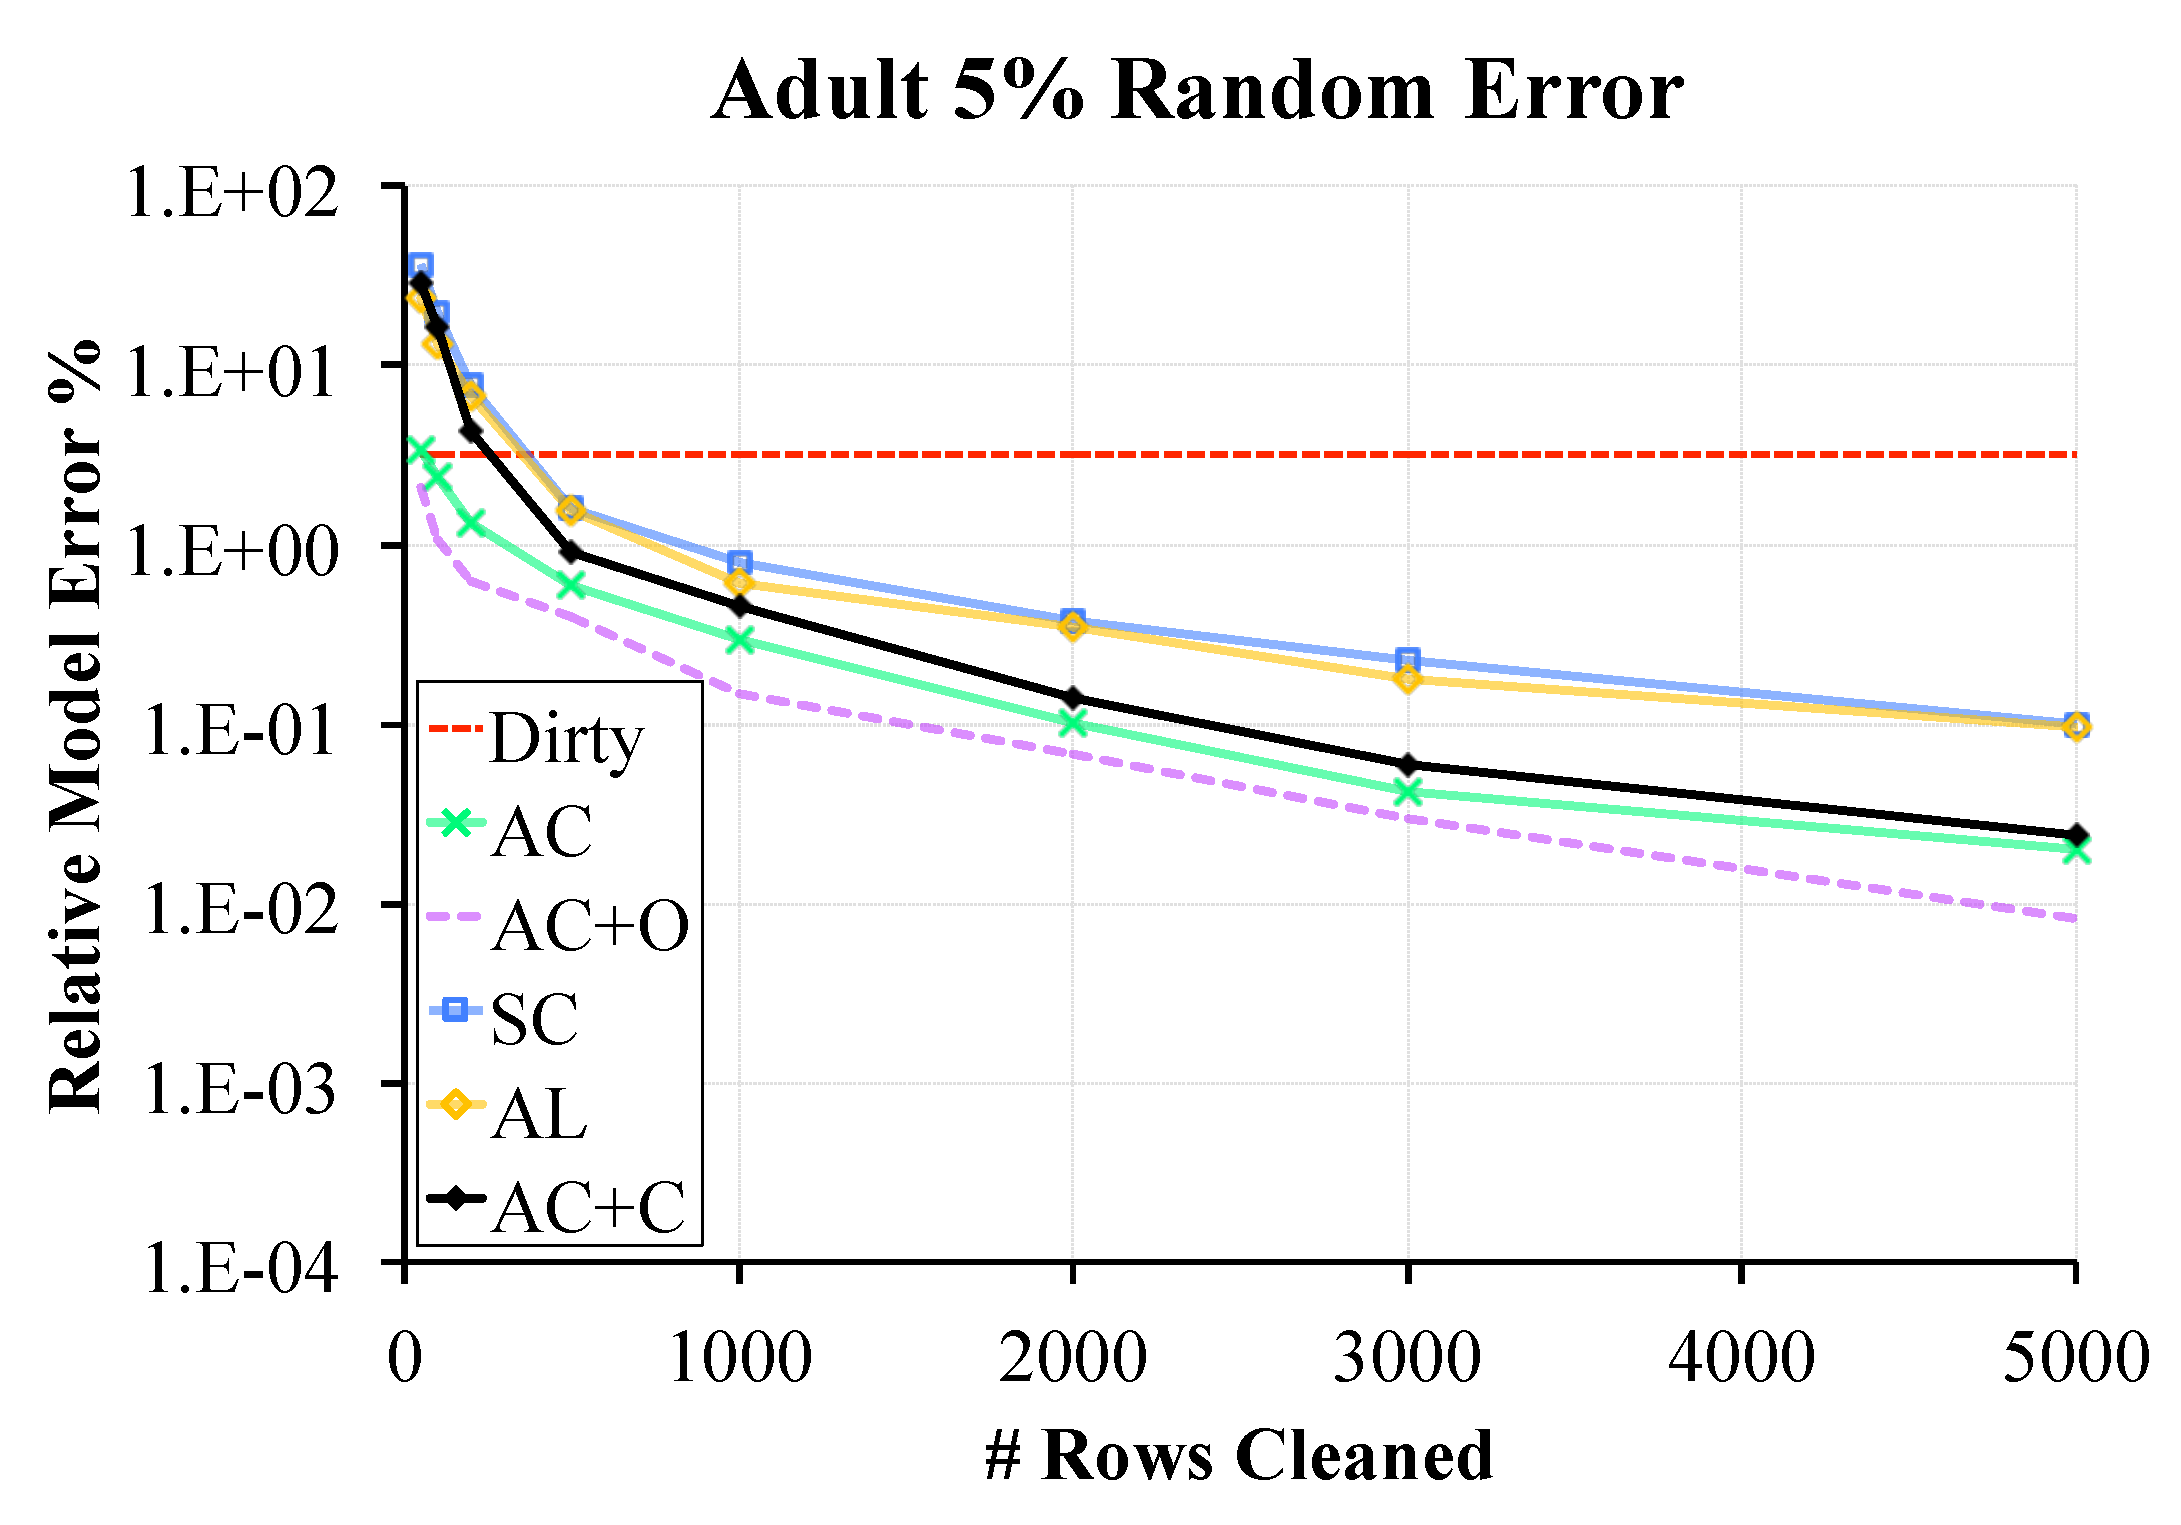
\includegraphics[width=0.48\columnwidth]{exp/exp11b.pdf}
 \caption{While initially \sys is comparable in performance to Active Learning, as the classifier improves, \sys converges faster than Active Learning and SampleClean. \label{pred-perf}}
\end{figure}

\subsubsection{3b. Classifiable Errors}
Using a classifier to partition errors depends on errors that can be classified.
For example, random errors that look like other data may be hard to learn.
As errors become more random, the classifier becomes increasingly erroneous.
We run an experiment where we start with the systematic errors described earlier.
With probability $p$, we increasingly make these errors more random.
We compare these results to AC-P where we do not partition the errors.
In Figure \ref{tradeoffs2}, we plot the error reduction using a classifier.
We find that when errors are about 40\% random then we reach a break even point
where the user is better of not partitiong the data since the errors introduced by incorrect classification are more than the error reductions.

\begin{figure}[ht!]
\centering
 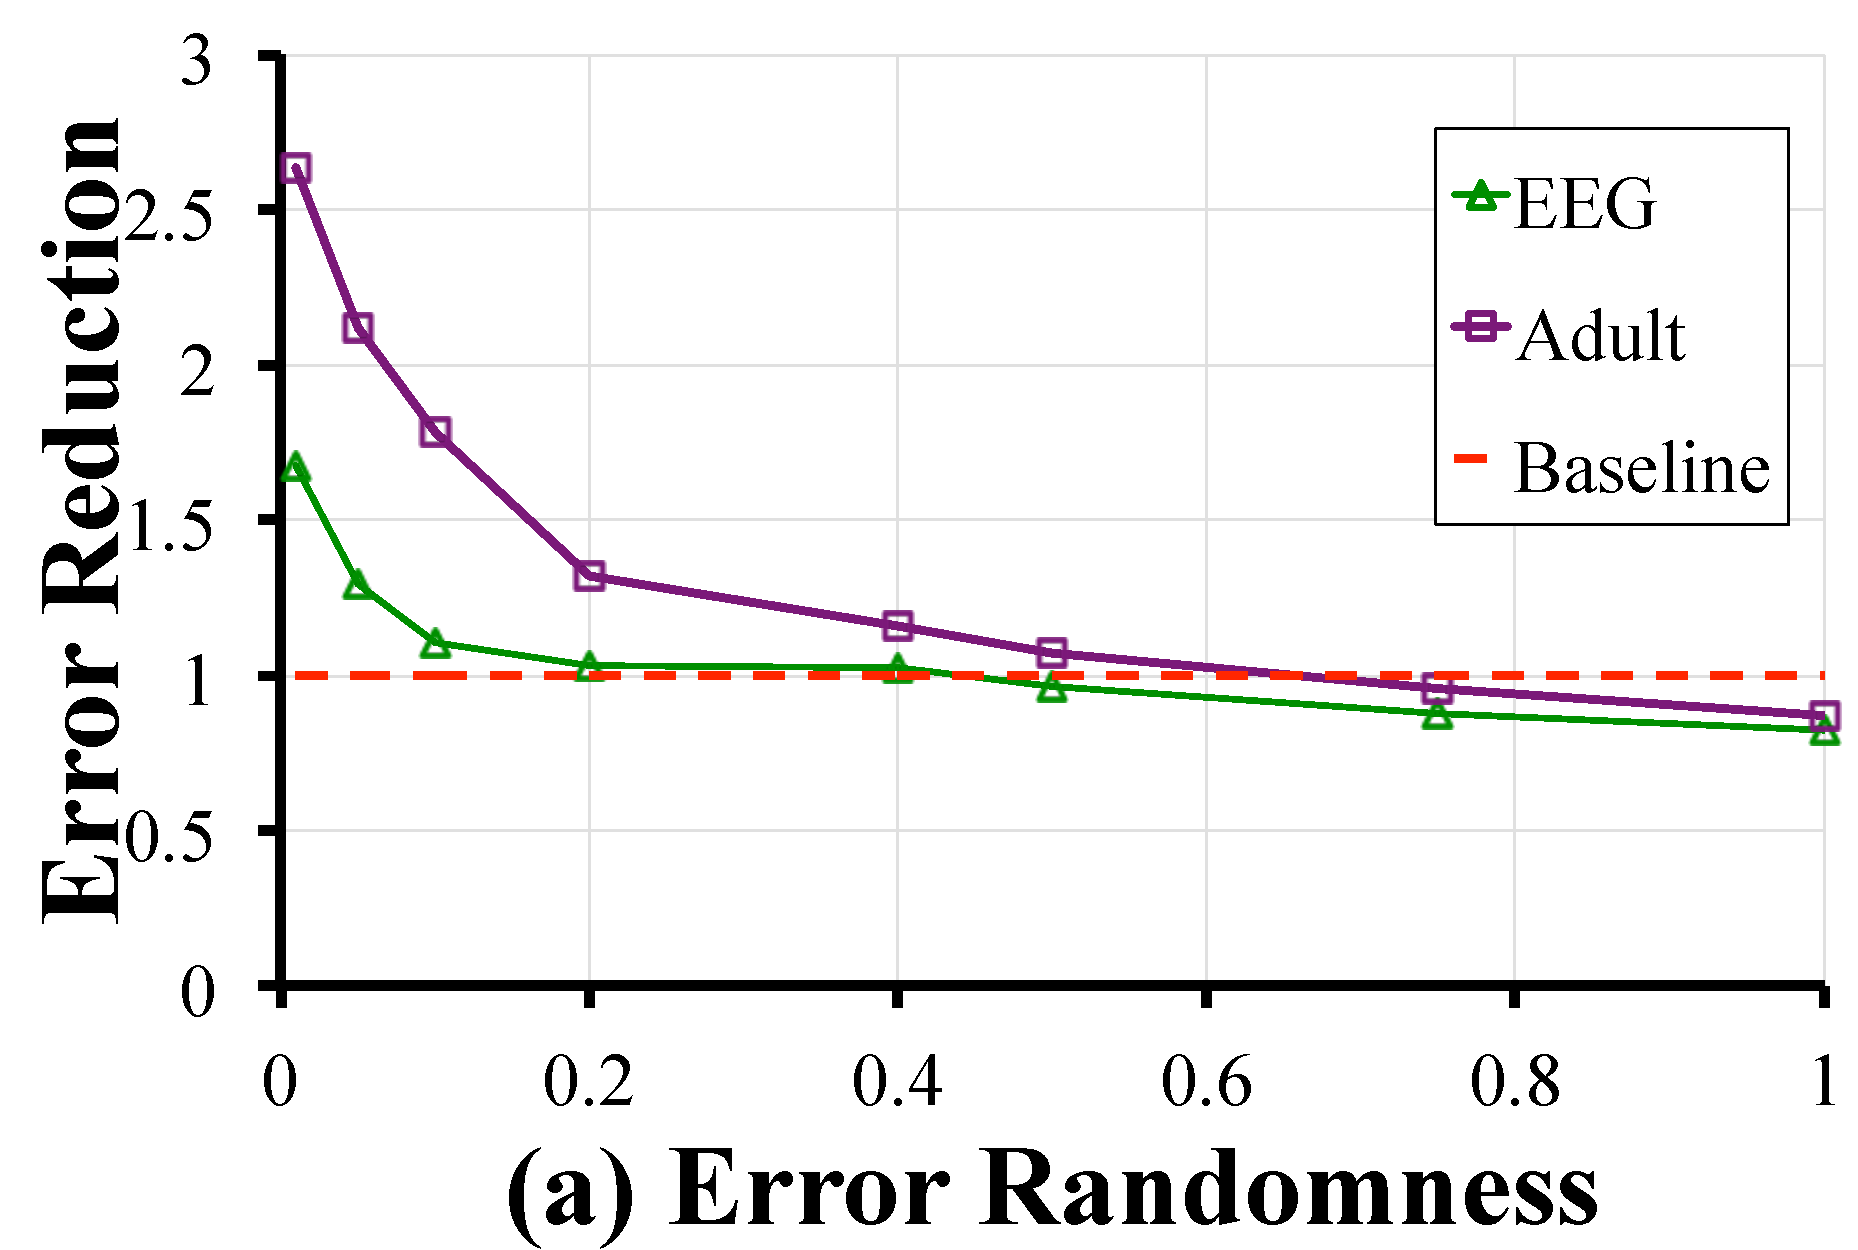
\includegraphics[scale=0.13]{exp/exp5a.pdf}
 \caption{Errors that are less random are easier to classify, and lead to more significant reductions in relative model error. \label{tradeoffs2}}
\end{figure}

\subsection{Experiment 4. Price of a Scan}
In our fourth set of experiments, we evaluate one of the computational premises of our work.
We argue that the price of a scan of data is cheap compared to data cleaning.
The overheads of partioning the dirty and clean data and calculating the sampling distribution should be small in comparison to the faster convergence of our model.
\reminder{How do we quantify the costs of data cleaning?} 

\subsection{Real Scenarios}
\reminder{Value Filling: MNIST}

\begin{figure*}[t]
\centering
 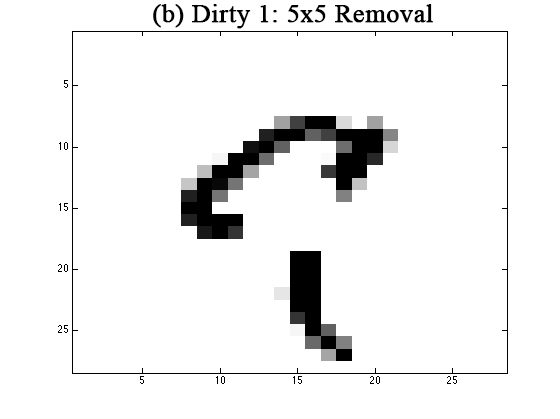
\includegraphics[scale=0.25]{exp/5x5removal.png}
 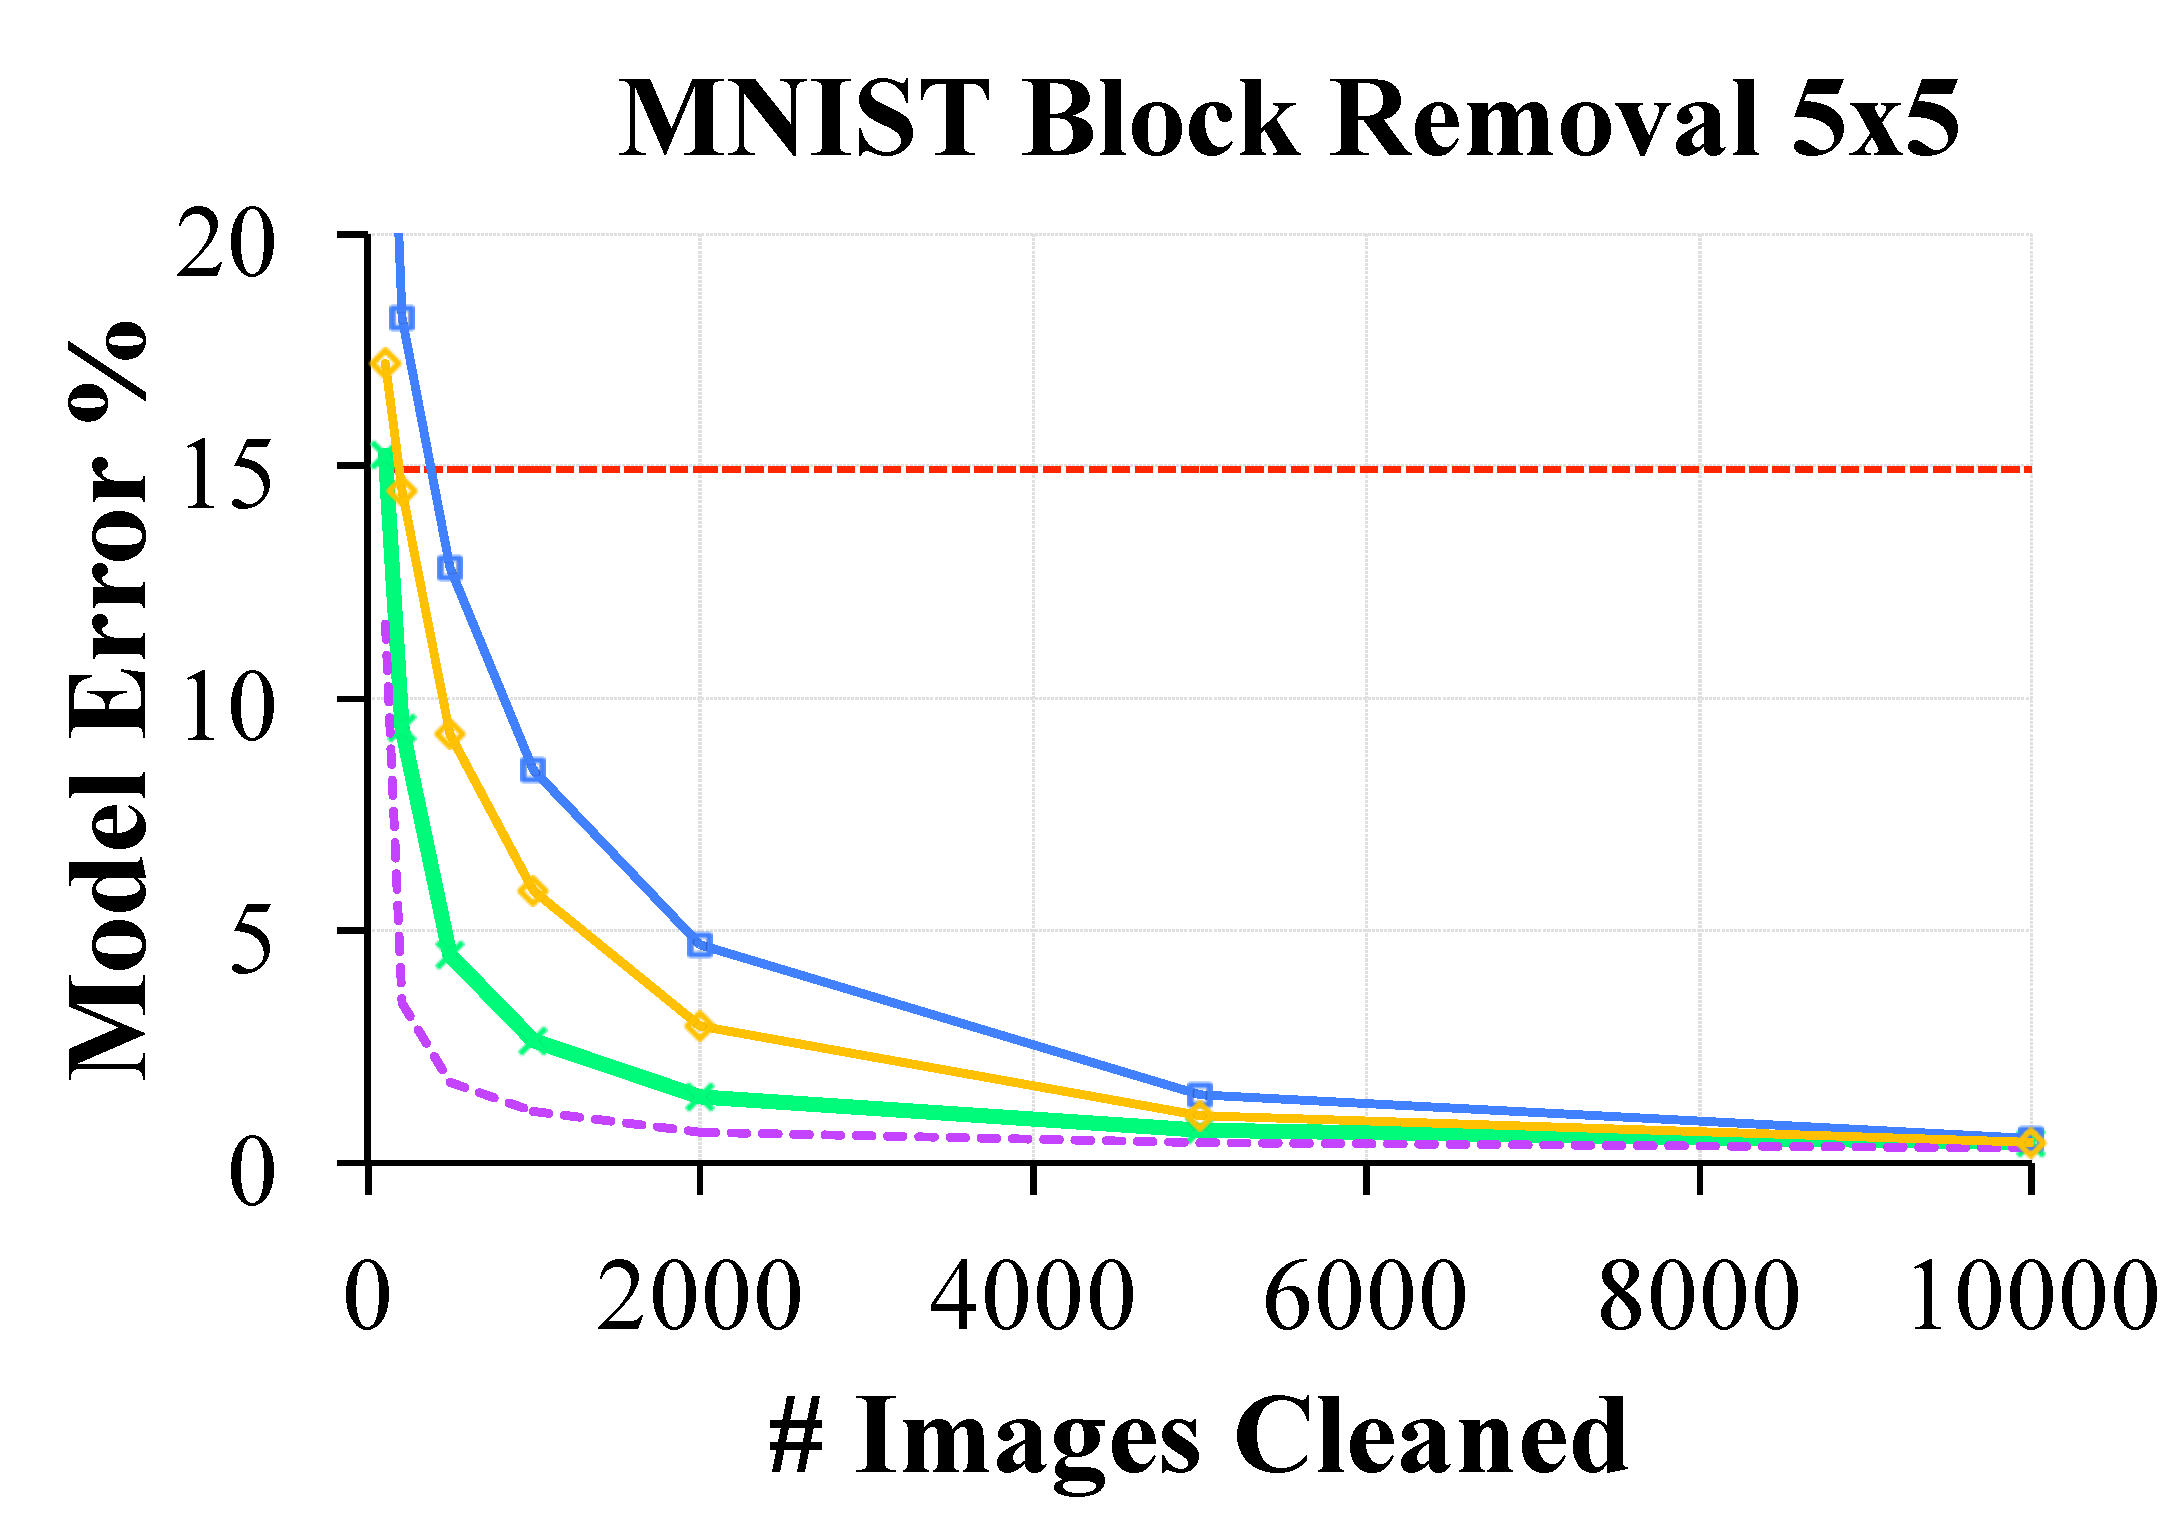
\includegraphics[scale=0.15]{exp/exp7a.pdf}
 \caption{One experiment with MNIST}
\end{figure*}

\reminder{CFD: Adult}
%
\section{Conclusion}
The growing popularity of predictive models (e.g., classifiers) in data analytics adds additional challenges in managing dirty data with mixing dirty and clean data, sensitivity to sampling, and sparsity.
\sys is a framework that utilizes data cleaning to mitigate systematic errors with progressive data cleaning.
The key insight is that an important class of predictive models, called convex loss models (e.g., linear regression and SVMs), can be simultaneously trained and cleaned.
Consequently, there are provable guarantees on the convergence and error bounds of \sys.  
\sys also includes numerous optimizations such as: using the information from the model to inform data cleaning on samples, dirty data detection to avoid sampling clean data, and batching together updates on already clean data.
The experimental results are promising as they suggest that these optimizations can significantly reduce data cleaning costs when errors are sparse and cleaning budgets are small.
Techniques such as Active Learning and SampleClean are not optimized for the sparse low-budget setting, and \sys achieves models of similar accuracy for significantly less records cleaned.
\vspace{-1em}

\bibliographystyle{abbrv}
%\scriptsize
\fontsize{7.8pt}{8.2pt} \selectfont
\bibliographystyle{abbrv}
\bibliography{ref} 

%%\section{Appendix}
\section{Set-of-Records Cleaning Model}\label{set-of-r}
In paper, we formalized the analyst-specified data cleaning as follows.
We take the sample of the records $S_{dirty}$, and apply data cleaning $C(\cdot)$.
$C$ is applied to a record and produces the clean record:
\[
S_{clean} = \{C(r) : \forall r \in S_{dirty}\}
\]
The record-by-record cleaning model is a formalization of the costs of data cleaning where each record has the same cost to clean and this cost does not change throughout the entire cleaning session.
There are, however, some cases when cleaning the first record of a certain type of corruption is expensive but all subsequent records are cheaper.

\begin{example}\label{app-ex1}
In most spell checking systems, when a misspelling is identified, the system gives an option to fix all instances of that misspelling.
\end{example}

\begin{example}\label{app-ex2}
In inconsistency problems, when an inconsistent value is identified all other records with the same inconsistency can be efficiently fixed.
\end{example}

This model of data cleaning can fit into our framework and we formalize it as the ``Set-of-Records" model as opposed to the ``Record-by-Record" model. 
In this model, the cleaning function $C(\cdot)$ is not restricted to updating only the records in the sample.
$C(\cdot)$ takes the entire dirty sample as an argument (that is the cleaning is a function of the sample), the dirty data, and updates the entire dirty data:
\[
R'_{dirty} = C(S_{dirty},R_{dirty})
\]
we require that for every record $s \in S_{dirty}$, that record is completely cleaned after applying $C(\cdot)$, giving us $S_{clean}$.
Records outside of $S_{dirty}$ may be cleaned on a subset of dirty attributes by $C(\cdot)$.
After each iteration, we re-run the detector, and move any $r \in R'_{dirty}$ that are clean to $R_{clean}$.
Such a model allows us to capture data cleaning operations such as in Example \ref{app-ex1} and Example \ref{app-ex2}.

\section{Stochastic Gradient Descent}\label{appsgd}

Stochastic Gradient Descent converges for a suitably chosen step size if the sample gradients are unbiased estimates of the full gradient. 
The first problem is to choose weights $\alpha$ and $\beta$ (to average already clean and newly cleaned data) such that the estimate of the gradient is unbiased. 
%SGD will converge when the estimate is unbiased and the step-size is chosen appropriately.
The batch $S_{dirty}$ is drawn only from $R_{dirty}$.
Since the sizes of $R_{dirty}$ and its complement are known, it follows that the gradient over the already clean data $g_C$ and the recently cleaned data $g_S$ can be combined as follows:
\[
g(\theta^{t}) = \frac{\mid R_{dirty} \mid \cdot g_S + \mid R_{clean} \mid \cdot g_C  }{\mid R \mid}
\]
Therefore,
\[
\alpha = \frac{\mid R_{clean} \mid}{\mid R \mid}, \beta = \frac{\mid R_{dirty} \mid}{\mid R \mid}
\]

\begin{lemma}
The gradient estimate $g(\theta)$ is unbiased if $g_S$ is an unbiased estimate of:
\[
\frac{1}{\mid R_{dirty} \mid} \sum g_i(\theta)
\]
\end{lemma}
\begin{proof}[Sketch]
\[
\mathbb{E}(\frac{1}{\mid R_{dirty} \mid} \sum g_i(\theta)) = \frac{1}{\mid R_{dirty} \mid} \cdot \mathbb{E}(\sum g_i(\theta)))
\]
By symmetry, 
\[
\mathbb{E}(\frac{1}{\mid R_{dirty} \mid} \sum g_i(\theta)) = g(\theta)
\]
\[
\mathbb{E}(\frac{1}{\mid R_{dirty} \mid} \sum g_i(\theta)) = \frac{\mid R_{dirty} \mid \cdot g_S + \mid R_{clean} \mid \cdot g_C  }{\mid R \mid}
\]
\end{proof}

The error bound discussed in Proposition 2 can be tightened for a class of models called strongly convex (see \cite{bertsekas2011incremental} for a defintion). 

\begin{proposition}
For a strongly convex loss, a batch size $b$, and $T$ iterations, the convergence rate is bounded by $O(\frac{\sigma^2}{bT})$. 
\end{proposition}

\section{Non-convex losses}\label{non-convex}
We acknowledge that there is an increasing popularity of non-convex losses in the Neural Network and Deep Learning literature. 
However, even for these losses, gradient descent techniques still apply. 
Instead of converging to a global optimum they converge to a locally optimal value. 
Likewise, \sys will converge to the closest locally optimal value to the dirty model. 
Because of this, it is harder to reason about the results.
Different initializations will lead to different local optima, and thus, introduces a complex dependence on the initialization with the dirty model.
This problem is not fundemental to \sys and any gradient technique suffers this challenge for general non-convex losses, and we hope to explore this more in the future.

\section{Importance Sampling}\label{impsample-deriv}
This lemma describes the optimal distribution over a set of scalars:
\begin{lemma}\label{impsample}
Given a set of real numbers $A = \{a_1,...,a_n\}$, let $\hat{A}$ be 
a sample with replacement of $A$ of size k.
If $\mu$ is the mean $\hat{A}$, the sampling distribution that minimizes
 the variance of $\mu$, i.e., the expected square error, is $p(a_i) \propto a_i$.
\end{lemma}
Lemma \ref{impsample} shows that when estimating a mean of numbers with sampling, the distribution with optimal variance is sampling proportionally to the values.

The variance of this estimate is given by:
\[
Var(\mu) = \mathbb{E}(\mu^2)-\mathbb{E}(\mu)^2
\] 
Since the estimate is unbiased, we can replace $\mathbb{E}(\mu)$ with the average of $A$:
\[
Var(\mu) = \mathbb{E}(\mu^2)-\bar{A}^2
\]
Since $\bar{A}$ is deterministic, we can remove that term during minimization.
Furthermore, we can write $\mathbb{E}(\mu^2)$ as:
\[
\mathbb{E}(\mu^2) = \frac{1}{n^2}\sum_i^n \frac{a_i^2}{p_i}
\]
Then, we can solve the following optimization problem (removing the proportionality of $\frac{1}{n^2}$) over the set of weights $P=\{p(a_i)\}$:
\[
\min_{P} \sum_i^N \frac{a_i^2}{p_i}
\]
\[
\text{subject to: } P > 0, \sum P = 1
\]
Applying Lagrange multipliers, an equivalent unconstrained optimization problem is:
\[
\min_{P > 0,\lambda > 0} \sum_i^N \frac{a_i^2}{p_i} + \lambda \cdot (\sum P - 1)
\]
If, we take the derivatives with respect to $p_i$ and set them equal to zero:
\[
-\frac{a_i^2}{2 \cdot p_i^2} + \lambda = 0
\]
If, we take the derivative with respect to $\lambda$ and set it equal to zero:
\[
\sum P - 1
\]
Solving the system of equations, we get:
\[
p_i = \frac{\mid a_i \mid }{\sum_i \mid a_i \mid}
\]

\section{Linearization}\label{apptaylor}
If $d$ is the dirty value and $c$ is the clean value, the Taylor series approximation for a function $f$ is given as follows:
\[
f(c) = f(d) + f'(d)\cdot(d-c) + ...
\]
Ignoring the higher order terms, the linear term $f'(d)\cdot(d-c)$ is a linear function in each feature and label.
We only have to know the change in each feature to estimate the change in value.
In our case the function $f$ is the gradient $\nabla\phi$.
So, the resulting linearization is:
\[
\nabla\phi(x^{(c)}_i,y^{(c)}_i,\theta) \approx \nabla\phi(x,y,\theta) + \frac{\partial}{\partial X}\nabla\phi(x,y,\theta)\cdot (x - x^{(c)}) \]
\[+ \frac{\partial}{\partial Y}\phi(x,y,\theta)\cdot (y - y^{(c)})
\]
When we take the expected value:
\[
\mathbb{E}(\nabla\phi(x_{clean},y_{clean},\theta)) \approx \nabla\phi(x,y,\theta) + \frac{\partial}{\partial X}\nabla\phi(x,y,\theta)\cdot \mathbb{E}(\Delta x) \]
\[+ \frac{\partial}{\partial Y}\nabla\phi(x,y,\theta)\cdot \mathbb{E}(\Delta y)
\]
It follows that:
\[
\approx \nabla\phi(x,y,\theta) + M_x \cdot \mathbb{E}(\Delta x) + M_y \cdot \mathbb{E}(\Delta y)
\]
where $M_x = \frac{\partial}{\partial X}\nabla\phi$ and $M_y = \frac{\partial}{\partial Y}\nabla\phi$.
Recall that the feature space is $d$ dimensional and label space is $l$ dimensional.
Then, $M_x$ is an $d \times d$ matrix, and $M_y$ is a $d \times l$ matrix.
Both of these matrices are computed for each record.
$\Delta x$ is a $d$ dimensional vector where each component represents a change in that feature and $\Delta y$ is an $l$ dimensional vector that represents the change in each of the labels. 

This linearization allows \sys to maintain per feature (or label) average changes and use these changes to center the optimal sampling distribution around the expected clean value.
To estimate $\mathbb{E}(\Delta x)$ and $\mathbb{E}(\Delta y)$, consider the following for a single feature $i$:
If we average all $j=\{1,...,K\}$ records cleaned that have an error for that feature, weighted by their sampling probability:
\[
\bar{\Delta}_{xi} = \frac{1}{NK}\sum_{j=1}^K (x^{(d)}[i]-x^{(c)}[i])\times \frac{1}{p(j)}
\]
Similarly, for a label $i$:
\[
\bar{\Delta}_{yi} = \frac{1}{NK}\sum_{j=1}^K (y^{(d)}[i]-y^{(c)}[i])\times \frac{1}{p(j)}
\]

Each $\bar{\Delta}_{xi}$ and $\bar{\Delta}_{yi}$ represents an average change in a single feature.
A single vector can represent the necessary changes to apply to a record $r$:
For a record $r$, the set of corrupted features is $f_r,l_r$.
Then, each record $r$ has a d-dimensional vector $\Delta_{rx}$ which is constructed as follows:
\[
 \Delta_{rx}[i] = \begin{cases} 0 & i \notin f_r \\ 
\bar{\Delta}_{xi} & i \in f_r
\end{cases} 
\]
Each record $r$ also has an l-dimensional vector $\Delta_{ry}$ which is constructed as follows:
\[
 \Delta_{rx}[i] = \begin{cases} 0 & i \notin l_r \\ 
\bar{\Delta}_{yi} & i \in l_r
\end{cases} 
\]
Finally, the result is: 
\[p_{r}\propto\|\nabla\phi(x,y,\theta^{(t)}) + M_x \cdot \Delta_{rx} +  M_y \cdot \Delta_{ry}\|
\]

\section{Example $M_x$, $M_y$}\label{example-deriv}
\noindent\textbf{Linear Regression: }
\[
\nabla\phi(x,y,\theta) = (\theta^Tx - y)x
\]
For a record, $r$, suppose we have a feature vector $x$.
If we take the partial derivatives with respect to x, $M_x$ is:
\[
M_x[i,i] = 2x[i] + \sum_{i \ne j} \theta[j]x[j] - y 
\]
\[
M_x[i,j] = \theta[j]x[i]
\]
Similarly $M_y$ is:
\[
M_y[i,1] = x[i] 
\]

\vspace{0.5em}

\noindent\textbf{Logistic Regression: } 
\[
\nabla\phi(x,y,\theta) = (h(\theta^Tx) - y)x
\]
where
\[
h(z) = \frac{1}{1+e^{-z}}
\]
we can rewrite this as:
\[
h_{\theta}(x) = \frac{1}{1+e^{\theta^Tx}}
\]
\[
\nabla\phi(x,y,\theta) = (h_{\theta}(x) - y)x
\]
In component form,
\[
g = \nabla\phi(x,y,\theta)
\]
\[
g[i] = h_{\theta}(x)\cdot x[i] - yx[i]
\]
Therefore,
\[
M_x[i,i] = h_{\theta}(x)\cdot(1- h_{\theta}(x))\cdot \theta[i] x[i] + h_{\theta}(x) - y
\]
\[
M_x[i,j] = h_{\theta}(x)\cdot(1- h_{\theta}(x))\cdot \theta[j] x[i] + h_{\theta}(x)
\]
\[
M_y[i,1] = x[i] 
\]

\noindent\textbf{SVM: } 
\[
\nabla\phi(x,y,\theta) =
\begin{cases}      
-y\cdot\boldsymbol{x} \text{ if } y\cdot\boldsymbol{x}\cdot\theta \le 1 \\
0\ \text{ if } y\ \boldsymbol{x}\cdot\theta \geq 1      
\end{cases}
\]
Therefore,
\[
M_x[i,i] = \begin{cases}      
-y[i] \text{ if } y\cdot\boldsymbol{x}\cdot\theta \le 1 \\
0\ \text{ if } y\ \boldsymbol{x}\cdot\theta \geq 1      
\end{cases} 
\]
\[
M_x[i,j] = 0
\]
\[
M_y[i,1] = x[i] 
\]

\section{Aggregate Queries as Convex Losses}
\subsection{AVG and SUM queries}
\avgfunc, \sumfunc queries are a special case of the convex loss minimization discussed in the paper:
If we define the following loss, it is easy to verify the the optimal $\theta$ is the mean $\mu$:
\[
\phi = (x_{i} - \theta)^2
\]
with the appropriate scaling it can support $\avgfunc$, $\sumfunc$ queries with and without predicates.
Taking the gradient of that loss:
\[
\nabla\phi = 2(x_{i} - \theta)
\]
It is also easy to verify that the bound on errors is $O(\frac{\mathbb{E}((x-\mu)^2}{bT})$, which is essentially the CLT.
The importance sampling results are inutitive as well.
Applying the linearization:
\[
M_x = 2
\]
The importance sampling prioritizes points that it expects to be far away from the mean.

\subsection{MEDIAN}
Similarly, we can analyze the \medfunc query.
If we define the following loss, it is easy to verify the the optimal $\theta$ is the median $m$:
\[
\phi = \mid x_{i} - \theta\mid
\]
Taking the gradient of that loss:
\[
\nabla\phi = \text{1 if < m, -1 if > m}
\]
Applying the linearization:
\[
M_x = 0
\]
The intuitive result is that a robust query like a median does not need to consider estimation as the query result is robust to small changes.

\section{Experimental Comparison}
\subsection{Robust Logistic Regression}\label{rlogit}
We use the algorithm from Feng et al. for robust logistic regression.
\begin{enumerate}
\item Input: Contaminated training samples $\{(x_1, y_1), . . . ,(x_{n}
, y_{n})\}$ an upper bound on the number of outliers n, number of inliers n and sample dimension p.
\item Initialization: Set \[T = 4\sqrt{\log p/n + \log n/n}\]
\item Remove samples $(xi
, yi)$ whose magnitude satisfies $\|x_i\| \ge T$.
\item Solve regularized logistic regression problem.
\end{enumerate}

\subsection{Active Learning}\label{al}
There is a well established link between Active Learning and Online Gradient-based Algorithms \cite{guillory2009active}. 
To fairly evaluate an Active Learning methodology in these experiments, we run a gradient descent where examples are priortized by expected gradient length (explained in \cite{settles2010active}).
Ignoring the detection step, there are two differences between this algorithm and the one we propose.
First, we calculate the gradient with respect to the an estimate of the clean data, and second we sample rather than using a deterministic ordering.
While such Active Learning algorithms have been studied in the Learning Theory community, they have not been adopted in data cleaning or crowdsourcing research.
Typical algorithms include uncertainty sampling, where a classifier prioritized data closest to the margin.
However, algorithms such as uncertainty sampling focus on the narrow problem of label acquisition in hyperplane classifiers; a problem too narrow for application in this setting.

\section{Dollars For Docs Setup}\label{dfd-errors}
The dollars for docs dataset has the following schema:
\begin{lstlisting}[mathescape,basicstyle={\scriptsize}]
Contribution(pi_speciality$\textrm{,}$ drug_name$\textrm{,}$ device_name$\textrm{,}$
corporation$\textrm{,}$ amount$\textrm{,}$ dispute$\textrm{,}$ status)
\end{lstlisting}
To flag suspect donations, we used the \texttt{status} attribute.
When the \texttt{status} was ``covered" that means it was an allowed contribution under the researcher's declared protocol.
When the \texttt{status} was ``non-covered" that means it was a disallowed contribution under the researcher's declared protocol.
The rest of the textual attributes were featurized with a bag-of-words model, and the numerical amount and dispute attributes were treated as numbers.

We cleaned the entire Dollars for Docs dataset upfront to be able to evaluate how different budgeted data cleaning strategies compare to cleaning the full data.
To clean the dataset, we loaded the entire data 240089 records into Microsoft Excel. We identified four broad classes of errors:
\vspace{0.25em}

\noindent \textbf{Corporations are inconsistently represented: } ``Pfizer", ``Pfizer Inc.", ``Pfizer Incorporated".

\vspace{0.25em}

\noindent \textbf{Drugs are inconsistently represented: } ``TAXOTERE  DOCETAXEL -PROSTATE CANCER" and ``TAXOTERE"

\vspace{0.25em}

\noindent \textbf{Label of covered and not covered are not consistent: } ``No", ``Yes",``N", ``This study is not supported", ``None", ``Combination"

\vspace{0.25em} 

\noindent \textbf{Research subject must be a drug OR a medical device and not both: } ``BIO FLU QPAN H7N9AS03 Vaccine" and ``BIO FLU QPAN H7N9AS03 Device"

\vspace{0.5em} 

To fix these errors, we sorted by each column and merged values that looked similar and removed inconsistencies as in the status labels. 
When there were ambiguities, we refered to the drug company's website and whitepapers.
When possible, we used batch data transformations, like find and replace (i.e. the Set-of-Records model).
In all, 44234 records had some error and full data cleaning required about 2 days of efforts.

Once cleaned, in our experiment, we encoded the 4 problems as data quality constraints.
To fix the constraints, we looked up the clean value in the dataset that we cleaned up front.

\vspace{0.25em}

\noindent \textbf{Rule 1: } Matching dependency on corporation (Weighted Jaccard Similarity $>$ 0.8).

\vspace{0.25em}

\noindent \textbf{Rule 2: } Matching dependency on drug (Weighted Jaccard Similarity $>$ 0.8).

\vspace{0.25em}

\noindent \textbf{Rule 3: } Label must either be ``covered" or ``not covered".

\vspace{0.25em} 

\noindent \textbf{Rule 4: } Either drug or medical device should be null.

\vspace{0.5em}

\section{MNIST Setup}
We include visualization of the errors that we generated for the MNIST experiment.
We generated these errors in MATLAB by taking the grayscale version of the image (a $64\times 64$ matrix) and corrupting them by block removal and fuzzying.

\begin{figure}[ht]
\centering
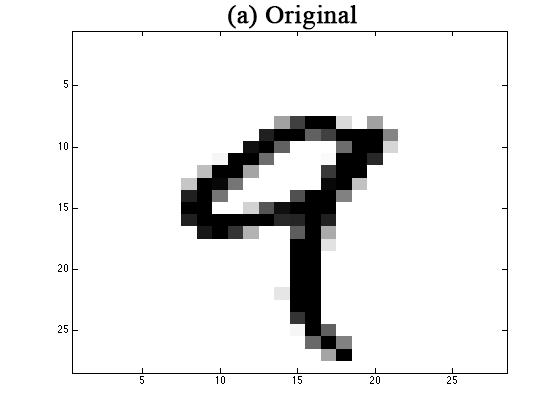
\includegraphics[scale=0.20]{exp/original.png}
 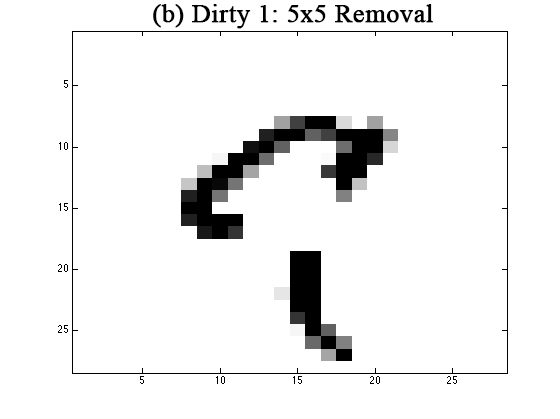
\includegraphics[scale=0.20]{exp/5x5removal.png}
 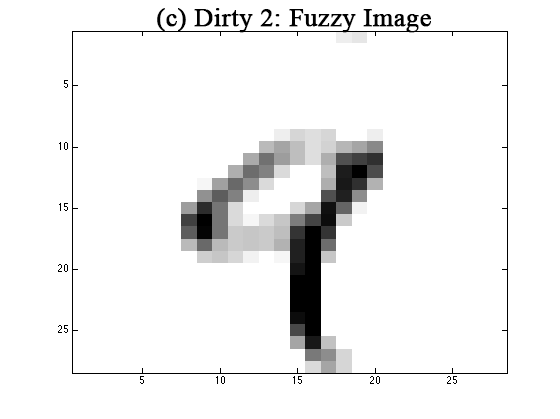
\includegraphics[scale=0.20]{exp/fuzzy.png}
 \caption{We experiment with two forms of corruption in the MNIST image datasets: 5x5 block removal and making the images fuzzy. Image (a) shows an uncorrupted ``9", image (b) shows one corrupted with block removal, and image (c) shows one that is corrupted with fuzziness. \label{mnist-corr}}
\end{figure}

\end{document}